\cotefile{16}
\scanpage{1}
\figure{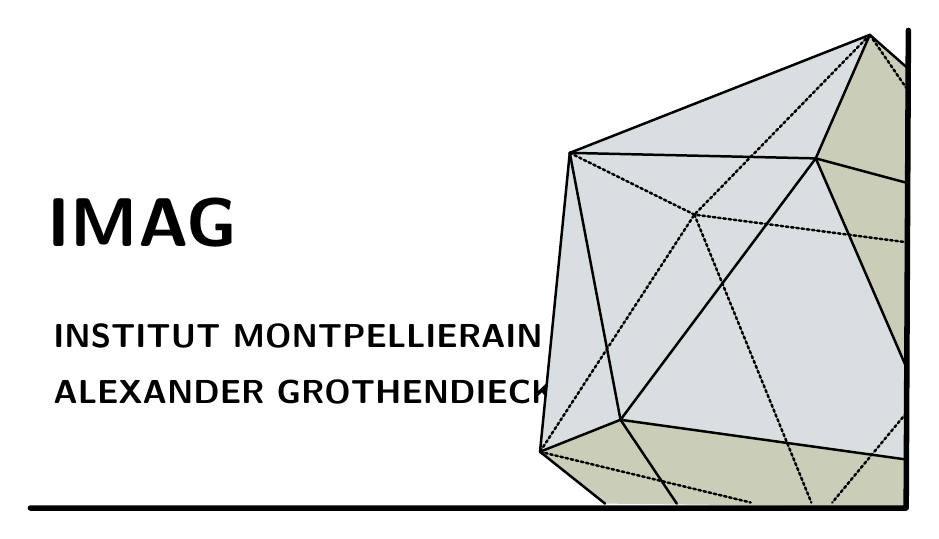
\begin{tikzpicture}[x=0.014cm,y=-0.014cm,line join=round,line cap=round]
\node[anchor=west,font=\sffamily\bfseries\fontsize{66}{72}\selectfont] at (15,202) {IMAG};
\node[anchor=west,font=\sffamily\bfseries\fontsize{12}{14}\selectfont] at (20,305) {INSTITUT MONTPELLIERAIN};
\node[anchor=west,font=\sffamily\bfseries\fontsize{12}{14}\selectfont] at (20,356) {ALEXANDER GROTHENDIECK};
\fill[fill={rgb,255:red,217;green,223;blue,224}] (497,139)--(769,32)--(720,144)--(543,381)--(470,410)--cycle;
\fill[fill={rgb,255:red,202;green,205;blue,184}] (769,32)--(802,61)--(802,333)--(720,144)--cycle;
\fill[fill={rgb,255:red,217;green,223;blue,224}] (720,144)--(802,333)--(802,417)--(543,381)--cycle;
\fill[fill={rgb,255:red,202;green,205;blue,184}] (543,381)--(802,417)--(802,460)--(529,457)--(470,410)--cycle;
\draw[line width=0.9pt] (497,139)--(769,32)--(802,61);
\draw[line width=0.9pt] (497,139)--(720,144)--(802,166);
\draw[line width=0.9pt] (769,32)--(720,144)--(802,333);
\draw[line width=0.9pt] (720,144)--(543,381)--(802,417);
\draw[line width=0.9pt] (497,139)--(470,410)--(543,381)--(594,457);
\draw[line width=0.9pt] (497,139)--(543,381);
\draw[line width=0.9pt] (470,410)--(529,457);
\draw[densely dotted,line width=0.9pt] (769,32)--(610,195)--(470,410);
\draw[densely dotted,line width=0.9pt] (769,32)--(802,80);
\draw[densely dotted,line width=0.9pt] (497,139)--(610,195)--(802,220);
\draw[densely dotted,line width=0.9pt] (610,195)--(716,456);
\draw[densely dotted,line width=0.9pt] (470,410)--(661,456);
\draw[densely dotted,line width=0.9pt] (802,375)--(735,456);
\draw[line width=2pt] (8,461)--(802,461)--(804,28);
\end{tikzpicture}}

\scanpage{3}
\mspage{1}
\uline{Sur certains anneaux gradués}

\inserted{Soit $k$ anneau (\unsure{comm.}) \unsure{fixé|fixe}.}

1. Soit \deleted{$k$ un anneau,} $M^*$ un $k$-module gradué\inserted{par $\mathbb Z$}, \inserted{à graduation finie}, $\mathcal E^*$ une \deleted{algèbre graduée}\inserted{sous-anneau de l'anneau} d'endomorphismes \inserted{du module \unsure{non-gradué} \unsure{(le produit)}} de $M^*$. On désigne par $\pi_i$ la projection canonique de $M^*$ sur $M^i$. \deleted{et} On suppose que l'on a :
\[
\pi_i\in\mathcal E^*\quad\text{pour tout }i
\tag{\unsure{1.2}}
\]
Cela implique que $\mathcal E^*$ est une \uline{sous-}\deleted{\uline{algèbre}}\inserted{anneau} graduée de l'algèbre graduée \deleted{des} $\operatorname{End}(M^*)$ [dont la graduation est définie, si $\nu\in\mathbb Z$, par
\[
\operatorname{End}^{(\nu)}(M)=\sum\operatorname{Hom}(M^i,M^{i+\nu})
\]
ou de façon équivalente
\[
\operatorname{End}^{(\nu)}(M)=\sum_i\pi_{i+\nu}\operatorname{End}(M^*)\pi_i,
\]
la composante homogène de degré $\nu$ d'un endomorphisme $u$ de $M^*$ étant
\[
\deleted{\unsure{u}}\quad\operatorname{pr}_{\nu}(u)=\sum_i\pi_{i+\nu}u\pi_i.
\]
La graduation de $\mathcal E^*$ est définie \inserted{\unsure{intrinsèque|intrinsèquement}}, en termes de la \deleted{\unsure{par}} donnée des $\pi_i$, par
\[
\left\{\begin{aligned}
\text{\textcircled{a}}\quad&\boxed{\mathcal E^{(\nu)}=\sum_i\pi_{i+\nu}\mathcal E^*\pi_i}\,,\\
\text{\textcircled{b}}\quad&\operatorname{pr}_{\nu}^{\mathcal E}u=\sum_i\pi_{i+\nu}u\pi_i
\end{aligned}\right.
\tag{\unsure{1.3}}
\]
\margin{et $(1.4.)\quad u\in\mathcal E^{(\nu)}\Longleftrightarrow u\pi_i=\pi_{i+\nu}u$ pour tt $i$\par
$\deleted{\unsure{\Longleftrightarrow u=\pi_{i+\nu}u\pi_i}}$}
\margin{\figure{\begin{tikzpicture}[x=1cm,y=1cm]
\node[anchor=west] at (9.8,1.7) {Noter les relations};
\node[anchor=west] at (.2,.8) {$(1.1)$};
\node[anchor=west] at (.2,.25) {\deleted{Notons}};
\node[anchor=west] at (2.1,.55) {$\left\{\begin{aligned}\pi_i^2&=\pi_i\\\pi_i\pi_j&=0\quad\text{si }i\neq j\\\sum\pi_i&=1\end{aligned}\right.$};
\draw[draw=brown!60!black] (.25,1.35) .. controls (-.1,1.15) and (-.35,.25) .. (.05,.05) .. controls (2,-.4) and (8,-.2) .. (11.5,.1) .. controls (13.8,.2) and (14.2,1.7) .. (13.2,2.0) .. controls (11.5,2.15) and (6.8,1.2) .. (.65,1.32);
\draw[draw=brown!60!black] (.3,1.15)--(.1,.65);
\draw[draw=brown!60!black] (.1,.6) circle (.055);
\end{tikzpicture}}}

2. Soit $\mathcal E^*$ une \deleted{$k$-algèbre}\inserted{anneau} graduée, et soient $\pi_i$ ($i\in\mathbb Z$) des éléments de $\mathcal E$, \inserted{nuls sauf un nb fini.} A quelles conditions les formules $(\unsure{1.3})$ définissent-elles
\mspage{\unsure{2}}

\scanpage{4}
\mspage{2}
sur $\unsure{\mathcal E^*|\mathcal E^{(\nu)}}$ une structure d'\deleted{\unsure{algèbre}}\inserted{anneau} graduée ?

Il suffit que l'on ait les relations $(1.1)$
\[
\deleted{\unsure{*}}\quad\left\{\begin{aligned}
\pi_i^2&=\pi_i\\
\pi_i\pi_j&=\pi_j\pi_i=0\quad\text{si }i\neq j\\
\sum\pi_i&=1
\end{aligned}\right.
\]
qui impliquent que les $\operatorname{pr}_{\nu}^{\mathcal E}$ définis par $(1.2.)$ sont des projections deux à deux orthogonales de somme $1$, donc que les $\mathcal E^{(\nu)}$ définissent bien une graduation \inserted{de $k$-modules} sur $\unsure{\mathcal E^{(\nu)}|\mathcal E^*}$, \deleted{puis}\inserted{et} que
\[
\mathcal E^{(\nu)}\mathcal E^{(\nu')}\subset\mathcal E^{(\nu\unsure{-|+}\nu')}.
\]
\margin{on peut remplacer $\mathbb Z$ par un \uline{\unsure{groupe|gr.}} quelconque}
Noter aussi que $(1.4.)$ que $(1.4)$ est valable, car \deleted{on a aussi la décomposition}
\[
\deleted{u=\sum_{ij}\pi_j u\pi_i}
\]
\deleted{\unsure{d'où} \unsure{la relation}}
\[
\deleted{\pi_{i+\nu}u\pi_i=\unsure{\pi_{i+\nu}|\pi_j}u\pi_i}
\qquad\inserted{\unsure{\mathcal E_i^j}}
\]
\[
\left\{\begin{aligned}
\mathcal E&=\bigoplus_{i,j}\pi_j\mathcal E\pi_i\\
\operatorname{pr}_{i,j}(u)&=\pi_j u\pi_i
\end{aligned}\right.
\qquad\text{donc }u=\sum_{\alpha,\beta}\pi_\beta u\pi_\alpha
\]
et la relation $u\pi_i=\pi_{i+\nu}u$ implique, puisque
\[
u\pi_i=\sum_\beta\pi_\beta u\pi_i,\quad\text{et}\quad
\pi_{\unsure{j|i}+\nu}u=\sum_{\unsure{i|\alpha}}\pi_{\unsure{j|i}+\nu}u\pi_\alpha,
\]
que
\[
\pi_\beta u\pi_i=0\quad\text{si }\beta\neq i+\nu.
\]
\margin{\figure{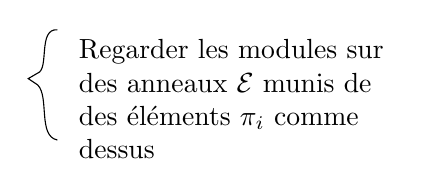
\begin{tikzpicture}[x=1cm,y=1cm]
\node[anchor=north west,align=left] at (.4,1.4) {Regarder les modules sur\\\deleted{des} anneaux $\mathcal E$ munis \deleted{\unsure{de}}\\des éléments $\pi_i$ comme\\dessus};
\draw (.25,1.4) .. controls (0,1.42) and (.15,.9) .. (0,.85) --(-.12,.78) --(0,.7) .. controls (.15,.55) and (0,.05) .. (.25,0);
\end{tikzpicture}}}

3. \deleted{Nous \unsure{voulons}} Partons enfin d'une \deleted{algèbre}\inserted{anneau} graduée $\mathcal E^*$ \deleted{sur $k$}, et posons nous la question de l'existence et \uline{l'unicité} d'une famille $(\pi_i)_{i\in\mathbb Z}$ d'éléments de $\mathcal E^*$, \inserted{satisfaisant $(1.1.)$} définissant la graduation, par $(1.3.)$ (donc par $(1.4)$). On \deleted{\unsure{supp}} suppose ici que
\mspage{3}

\scanpage{5}
\mspage{3}
\deleted{\unsure{les $\pi_i$ de degré zéro}, et que} l'on \unsure{voudra|considère} que
\figure{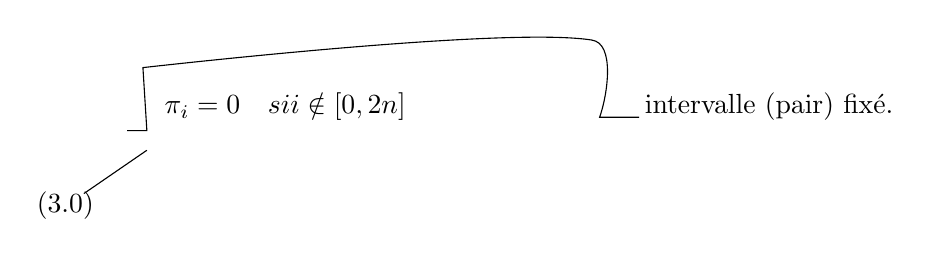
\begin{tikzpicture}[x=1cm,y=1cm]
\node[anchor=west] at (.8,.55) {$\pi_i=0\quad\text{si }i\notin[0,2n]$};
\node[anchor=west] at (6.9,.55) {intervalle \inserted{(pair)} fixé.};
\node[anchor=east] at (.15,-.7) {$(3.0)$};
\draw (.45,.25)--(.7,.25)--(.65,1.05) .. controls (2,1.2) and (5.4,1.55) .. (6.35,1.4) .. controls (6.65,1.36) and (6.55,.7) .. (6.45,.42)--(6.95,.42);
\draw (.7,0)--(-.1,-.55);
\end{tikzpicture}}
\deleted{\unsure{Supp}} On s'occupe ici de l'\uline{unicité}. \deleted{\unsure{Supposons, établie l'unicité}}

Notons d'abord que
\[
\mathcal E^0\ni u\quad\Longleftrightarrow\quad(u\pi_i=\pi_i u\quad\forall i)
\]
donc $\mathcal E^0$ est le commutant de la $k$-algèbre engendrée par les $\pi_i$. Donc les $\pi_i$ sont dans le centre $\unsure{Z|\mathfrak Z}(\mathcal E^0)$ de $\mathcal E^0$, et ce sont des projecteurs \inserted{mutuellement} orthogonaux de somme $1$ de cet anneau commutatif. Supposons déterminés déjà les $\pi_\alpha$ pour $\alpha\notin[i,2n-i]$, \inserted{$i<n$,} et déterminons $\pi_i$ et $\pi_{2n-i}$ [i.e. $\pi_\alpha$ pour $\alpha\notin[i+1,2n-i-1]$.]
\inserted{\figure{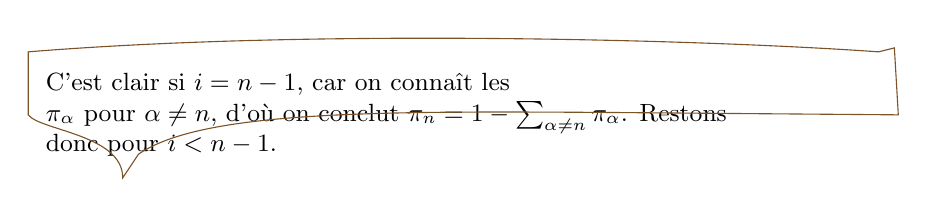
\begin{tikzpicture}[x=1cm,y=1cm]
\node[anchor=north west,align=left,font=\small] at (.2,.8) {C'est clair si $i=n-1$, car on connaît les\\$\pi_\alpha$ pour $\alpha\neq n$, d'où on conclut $\pi_n=1-\sum_{\alpha\neq n}\pi_\alpha$. \unsure{Restons}\\donc pour $i<n-1$.};
\draw[draw=brown!65!black] (.1,.95) .. controls (3.8,1.25) and (8.8,1.1) .. (10.9,.95) --(11.1,1.0)--(11.15,.15)--(7.5,.18) .. controls (4.5,.2) and (2.3,.2) .. (1.5,-.35) --(1.3,-.65) .. controls (1.3,-.1) and (.25,-.05) .. (.1,.15)--cycle;
\end{tikzpicture}}}
On connaît donc
\[
\varphi_i=\deleted{\unsure{1-\sum\pi_\alpha}}\left(1-\sum_{\alpha<i}\pi_{\unsure{i|\alpha}}\right)=\sum_{\alpha\geq i}\pi_\alpha,
\quad\text{et}\quad
\psi_{2n-i}=\left(1-\sum_{\alpha>2n-i}\pi_{\unsure{i|\alpha}}\right)=\sum_{\alpha\leq 2n-i}\pi_\alpha
\]
donc aussi la composante
\[
\unsure{ou}\quad\psi_{2n-i}\deleted{\unsure{\varphi}}\mathcal E^{2n-2i}\varphi_i
=\sum_\alpha\psi_{2n-i}\pi_{\alpha+(2n-2i)}\mathcal E\pi_\alpha\varphi_i\unsure{)}
\]
Or
\[
\pi_\alpha\varphi_i=\begin{cases}0&\text{si }\alpha<i\\\pi_\alpha&\text{si }\alpha\geq i\end{cases}
\quad\text{et}\quad
\psi_{2n-i}\pi_{\alpha+(2n-2i)}=
\begin{cases}
0&\text{si }\inserted{\alpha+(2n-2i)>2n-i}\quad\text{i.e. }\alpha>i\\
\pi_{\alpha+(2n-2i)}&\text{si }\inserted{\alpha\leq i}
\end{cases}
\]
donc le terme d'indice $\alpha$ de la somme $\sum$ est nul sauf si $\alpha=i$, auquel cas il est égal à
\[
\pi_{\unsure{i|\alpha}+(2n-2i)}\mathcal E\pi_i=\pi_{2n-i}\mathcal E\pi_i=\mathcal E_{2n-i,i}.
\]
Donc la connaissance des $\pi_\alpha$ pour $\alpha\notin[i,2n-i]$ implique la connaissance de $\mathcal E_{\deleted{\unsure{i,2n-i}}\inserted{2n-i,i}}$ \deleted{\unsure{Consid}}

La condition qui va impliquer l'unicité \deleted{\unsure{de}} de $\unsure{u_i|\pi_i}$,
\mspage{4}

\scanpage{6}
\mspage{4}
$\unsure{u_{2n-i}|\pi_{2n-i}}$ est \unsure{donc} la \deleted{\unsure{qui}} conjonction des suivantes :
\[
\begin{array}{l}(3.1.)_i\\[18pt](3.2)_i\end{array}
\quad\left.\begin{array}{l}\Bigl[
\bigl(u\in\unsure{\mathfrak Z|\mathcal Z}\mathcal E^0,\ \deleted{\unsure{\pi_\alpha u=0\ (\alpha\neq i),}}\ 
\figure{\begin{tikzpicture}[baseline=(e.base)]\node[draw,ellipse,inner sep=2pt] (e) {$\mathcal E_i^{2n-i}$};\end{tikzpicture}}u=0\bigr)
\Longrightarrow\deleted{u=0}\inserted{\pi_i u=0},\\[12pt]
\bigl(u\in\unsure{\mathfrak Z|\mathcal Z}\mathcal E^0,\ \deleted{\unsure{\pi_\alpha u=0\ (\alpha\neq2n-i),}}\ u\mathcal E_i^{2n-i}=0\bigr)
\Longrightarrow\deleted{u=0}\inserted{\pi_{2n-i}u=0}
\end{array}\right]
\]
En effet, la relation $(3.1.)$ implique que \deleted{$\unsure{\pi_i(\mathfrak Z\mathcal E^0)}$}\inserted{l'annulateur de $\pi_i$ dans $\unsure{\mathfrak Z|\mathcal Z}\mathcal E^0$} est l'idéal des $u\in\unsure{\mathfrak Z|\mathcal Z}\mathcal E^0$ tels que $\mathcal E_i^{2n-i}u=0$; or dans un anneau commutatif, un idempotent est connu quand on connaît son annulateur. De même pour $\pi_{2n-i}$, son annulateur dans $\unsure{\mathfrak Z|\mathcal Z}\mathcal E^0$ est formé des $u\in\unsure{\mathfrak Z|\mathcal Z}\mathcal E^0$ tels que $u\mathcal E_i^{2n-i}=0$.

En même temps, les conditions $(3.1.)_i$, $(3.2.)_i$ pour tt $i$, donnent un \deleted{condition} procédé pour déterminer de proche en proche les $\pi_i$.

\figure{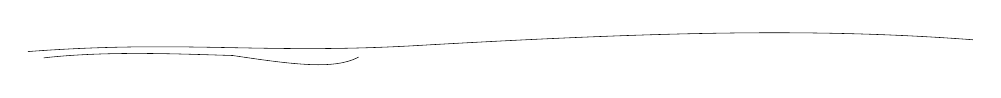
\begin{tikzpicture}[x=1cm,y=1cm]\draw[line width=.2pt] (0,0) .. controls (2,.15) and (3,-.04) .. (5,.08) .. controls (8,.25) and (10,.30) .. (12,.15);\draw[line width=.2pt] (.2,-.08) .. controls (1,.01) and (1.9,-.03) .. (2.6,-.05) .. controls (3.4,-.17) and (3.9,-.23) .. (4.2,-.07);\end{tikzpicture}}

4. Lorsque $\mathcal E^*$ est comme dans 1., une condition suffisante pour avoir $(3.1)_i$ \inserted{resp. $(3.2)_i$} est la \deleted{\unsure{suff}} suivante

$(\unsure{4.1})_i$ L'intersection des noyaux des $v:M^i\longrightarrow M^{2n-i}$, pour $v\in\mathcal E_i^{2n-i}$, est réduite à $0$.

$(4.2)_i$ La somme des images des $v:M^i\unsure{-|\longrightarrow}M^{2n-i}$, pour $v\in\mathcal E_i^{2n-i}$, est \deleted{\unsure{à}} égale à $M^{2n-i}$.

Ces deux conditions sont satisfaites si on a

$(4.3)_i$ Il existe \inserted{$v:M^i\unsure{-|\longrightarrow}M^{2n-i}$,} $v\in\mathcal E_i^{2n-i}$, qui est un isom. de
\mspage{5}

\scanpage{7}
\mspage{5}
façon équivalente, il existe un $v\in\mathcal E^{2n-2i}$, tel que le morphisme induit $v:M^i\unsure{-|\longrightarrow}M^{2n-i}$ soit un isomorphisme.

On peut transformer ceci de la façon suivante :
\[
\left\{\begin{aligned}
&\exists\ v_i\in\mathcal E^{2n-2i},\quad w_i\in\mathcal E^{-(2n-2i)},\quad\text{tels que l'on ait}\\
&(w_iv_i-1)\pi_i=0,\quad(v_iw_i-1)\pi_{2n-i}=0
\end{aligned}\right.
\tag*{$(4.4)_i$}
\]
Or, sans plus supposer que $\mathcal E^*$ se réalise à l'aide d'un $M^*$, on voit aussitôt que $(4.4)_i$ implique $(3.1)_i$ et $(3.2)_i$. En effet, quitte à remplacer $v,w$ par $v\pi_i=\pi_{2n-i}v$, $w\pi_{2n-i}=\pi_iw$, on peut supposer $v,w$ dans $\mathcal E_i^{2n-i}$, $\mathcal E_{2n-i}^i$. Si alors \deleted{\unsure{u}} $u\in\mathcal E^{(0)}$ est tel que $\mathcal E_i^{2n-i}u=0$, donc $vu=0$, on aura $wvu\pi_i\deleted{\unsure{=}}=0$ i.e. $wv\pi_i u=0$ donc $\pi_i u=0$ (car $wv\pi_i=\pi_i$). De $=$ pour $(3.2)_i$, en utilisant la deuxième relation $(\unsure{4.4})_i$.

\margin{\figure{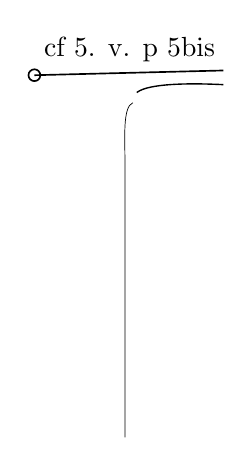
\begin{tikzpicture}[x=1cm,y=1cm]
\node[anchor=south west] at (0,4.65) {cf 5. v. p 5bis};
\draw[line width=.6pt] (0,4.6)--(2.4,4.66);
\draw[line width=.6pt] (0,4.6) circle (.075);
\draw[line width=.5pt] (1.3,4.38) .. controls (1.45,4.5) and (2.0,4.5) .. (2.4,4.48);
\draw[line width=.25pt] (1.25,4.25) .. controls (1.12,4.2) and (1.15,3.8) .. (1.15,3.5)--(1.15,0);
\end{tikzpicture}}}

\unsure{6}. Nous allons étudier de façon plus détaillée un cas où les conditions $(4.4)$ sont satisfaites. Pour ceci, partons encore de la situation $M^*$, \inserted{$\mathcal E^*$ sous-algèbre graduée de $\operatorname{End}(M^*)$,} et supposons qu'on ait un
\[
L\in\mathcal E^{(2)}
\tag{6.0}
\]
qui ait la propriété que
\mspage{6}

\scanpage{8}
\figure{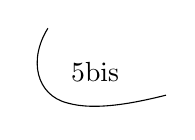
\begin{tikzpicture}[x=1cm,y=1cm]
\node at (.7,.45) {\mspage{5bis}};
\draw (.1,1.0) .. controls (-.15,.6) and (-.05,.15) .. (.35,.05) .. controls (.7,-.05) and (1.2,.05) .. (1.6,.15);
\end{tikzpicture}}
5. On peut aussi donner une condition d'\uline{existence} des $\pi_i$, liée aux conditions $(4.4)$. Pour ceci, on suppose que $\mathcal E$ est contenu dans un \unsure{sur-anneau|sous-anneau} gradué $\mathcal F$ [p.ex. \inserted{l'anneau} des endom. d'un $M^*$ comme dans 1.] pour lequel les $\pi_i$ satisfont $(1.1.)$ et les relations \unsure{correspondantes|correspondant} à $(1.3)$ (avec $\mathcal E$ remplacé par $\mathcal F$) sont satisfaites; \inserted{(et $(3.0)$: $\pi_i=0$ si $i\notin[0,2n]$)} Supposons que $\forall i$, la condition $(4.4)_i$ soit satisfaite, (avec $v_i,w_i\in\mathcal E$ bien sûr). On va en conclure que
\[
\pi_i\in\mathcal E\quad\text{pour tt }i.
\tag{5.1}
\]
\deleted{\unsure{Raisonnons par récurrence sur $i$.}}\inserted{Supposons prouvé \deleted{\unsure{que}} déjà $\pi_\alpha\in\mathcal E$ si $\alpha\notin[i,2n-i]$,} où $i<n$, et prouvons que l'on peut remplacer $i$ par $i+1$, \inserted{i.e. $\pi_i$ et $\pi_{2n-i}\in\mathcal E$.}\inserted{Trivial si $i=n-1$, supposons que $i\leq n-2$.}

Notons que, avec les notations de 3., \deleted{\unsure{on a}}\inserted{on a $\varphi_i,\psi_{2n-i}\in\mathcal E$, \unsure{d'où|donc}} \deleted{\unsure{remplaçons} $v_i,\inserted{w_i}$ par} \deleted{\unsure{alors}}\inserted{donc} $\psi_{2n-i}v_i\varphi_i$, $\varphi_iw_i\psi_{2n-i}\in\mathcal E$, i.e.
\[
\left\{\begin{aligned}
\inserted{v'_i={}}\psi_{2n-i}v_i\varphi_i&=\pi_{2n-i}v_i\pi_i\in\mathcal E\\
\inserted{w'_i={}}\varphi_iw_i\psi_{2n-i}&=\pi_iw_i\pi_{2n-i}\in\mathcal E
\end{aligned}\right.
\]
et \uline{comme} \deleted{\unsure{donc}}
\[
w'_iv'_i=\pi_iw_i\pi_{2n-i}v_i\pi_i
\inserted{\quad\text{car }w_i\pi_{2n-i}=\pi_iw_i}\]
\[
=\pi_i\pi_iw_iv_i\pi_i
\inserted{\quad\text{car }w_iv_i\pi_i=\pi_i}
=\pi_i^3=\pi_i.
\]
et de $=$ \deleted{$\unsure{=\pi_i}$} $v'_iw'_i=\pi_{2n-i}$, on conclut que $\pi_i\in\mathcal E$, $\pi_{2n-i}\in\mathcal E$.
\mspage{7}

\scanpage{9}
\mspage{6}
\[
L^{n-i}|M^i:\quad M^i\longrightarrow M^{2n-i}\quad\text{est un isom.}
\tag*{$(\unsure{6.1})_i$}
\]
Ceci implique déjà $(4.1)_i$ et $(4.2)_i$ donc $(3.1)_i$ et $(3.2)_i$; \inserted{\figure{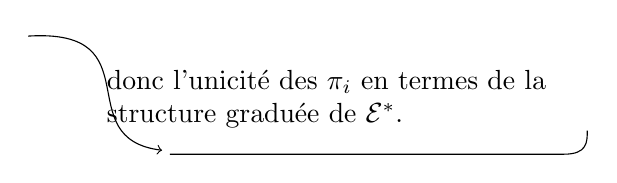
\begin{tikzpicture}[x=1cm,y=1cm]
\node[align=left,text width=6cm] at (1,0) {donc l'\uline{unicité} des $\pi_i$ en termes de la structure graduée de $\mathcal E^*$.};
\draw[->] (-3,.8) .. controls (-1.4,.9) and (-2.5,-.5) .. (-1.3,-.65);
\draw (-1.2,-.7) -- (3.8,-.7) .. controls (4.1,-.7) and (4.1,-.55) .. (4.1,-.4);
\end{tikzpicture}}} Supposons de plus

$(\unsure{6.2})_i$ L'inverse de l'isom. $(6.1)$ est \deleted{\unsure{dans $\mathcal E_{2n-i}^i$}} induit par un élément de $\mathcal E^{-(2n-2i)}$.

\deleted{\unsure{Ceci}} L'ensemble des deux conditions $(6.1)$ et $(6.2)$, équivalent [en termes intrinsèques à $\mathcal E^*$, muni de $L\in\mathcal E^2$ si on suppose déjà les $\pi_i\in\mathcal E^*$]
\[
\left\{\begin{aligned}
&\exists\ w_i\in\mathcal E^{-(2n-2i)}\quad\text{tel qu'on ait}\\
&(w_iL^{n-i}-1)\pi_i=0,\quad(L^{n-i}w_i-1)\pi_{2n-i}=0
\end{aligned}\right.
\tag*{$(6.3.)_i$}
\]
Cette condition à son tour (indépendamment de la donnée préliminaire d'un $M^*$) implique $(4.4)_i$, \deleted{et on a donc $(3.1)_i$ et $(3.2)_i$}, \figure{\begin{tikzpicture}[x=1cm,y=1cm]
\node[align=center] at (0,.55) {\inserted{(en vertu des\\ n° 4, 5)}};
\node at (2.4,.65) {\inserted{$\pi_i\in\mathcal E$ et,}};
\node at (.65,-.1) {donc};
\draw (-1.2,.5) .. controls (-1.5,-.15) and (-.9,.1) .. (0,.1) .. controls (.8,.1) and (1.25,.2) .. (1.3,-.3);
\draw (1.4,.5) .. controls (2,.5) and (1.9,-.1) .. (2,-.35) .. controls (1.8,.35) and (3,.3) .. (3.6,.6);
\end{tikzpicture}} l'\uline{unicité} des $\pi_i$ en termes des conditions $(1.1)$ et $(\unsure{1.7|1.3})$.

Revenons à $M^*$, et $L$ satisfaisant à $(6.1)_i$. Nous avons vu comment \deleted{la} cette condition implique la \uline{décomposition de} $M^*$ en termes \deleted{\unsure{can.}} de morceaux primitifs
\[
\left\{\begin{aligned}
M^i&\simeq P^i+LP^{i-2}+L^2P^{i-4}\quad\text{---}\\
M^{2n-i}&\simeq L^{n-i}P^i+L^{n-i+1}P^{i-2}\quad\text{---}
\end{aligned}\right.\qquad\bigg|\quad\text{si }i\leq n
\tag{\unsure{6.4}}
\]
On désigne par $\pi_{i,\alpha}$ la projection de $M^i$ sur $L^\alpha P^{i-2\alpha}$, par $\pi_{2n-i,\alpha}$ celle de $M^{2n-i}$ sur $L^{n-i+\alpha}P^{i-2\alpha}$,
\mspage{8}

\scanpage{10}
\mspage{7}
On a aussi l'hom. $\Lambda$ de degré $-2$, défini par
\[
\left\{\quad\unsure{\cdot\ \cdot\ \cdot\ \cdot\ \cdot\ \cdot}\right.
\tag{6.5}
\]
\uline{Théorème} Les conditions suivantes \inserted{(i) à (iii)} sont équivalentes

(i) Les conditions \inserted{$(6.1)_i$ et} $(6.2)_i$ pour tt $i$, et les $\pi_i\in\mathcal E$.

\deleted{\unsure{(ii)} [\unsure{Une graduation|La graduation} de $\mathcal E^*$ peut être définie par des $\pi'_i$, et \unsure{pour un|pour que} \deleted{\illegible{2}} \unsure{tel choix|tels que};]\par
\unsure{(ii)} \unsure{Les conditions} $(6.3)_i$ pour tt $i$ (avec $\pi_i$ \unsure{remplacé par} $\pi'_i$,....)}
\margin{\figure{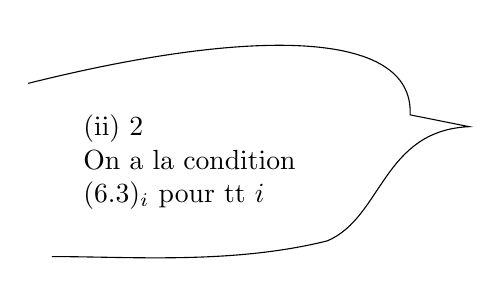
\begin{tikzpicture}[x=1cm,y=1cm]
\node[align=left,text width=4.2cm] at (0,0) {(ii) \deleted{\illegible{2}}\\On a la condition\\$(6.3)_i$ pour tt $i$};
\draw (-2.8,1) .. controls (0,1.7) and (2.1,1.7) .. (2.05,.6) -- (2.8,.45) .. controls (1.7,.4) and (1.7,-.7) .. (1,-1) .. controls (-.2,-1.3) and (-1.5,-1.2) .. (-2.5,-1.2);
\end{tikzpicture}}}

(iii) \deleted{L'hom.}\inserted{On a} \inserted{$(6.1)_i$ pour tt $i$, (\unsure{défin.|défini|définit} $\Lambda$) et}
\[
\uline{\Lambda\in\mathcal E^{(-2)}}
\tag{\unsure{6.6}}
\]
\deleted{\unsure{(iv)}} Ces conditions impliquent de plus

(iv) Les $\pi_{i,\alpha}$ sont dans $\mathcal E$, \deleted{les $\pi_i$ sont dans $\mathcal E$.}

(v) Les $\pi_i\in\mathcal E$, \inserted{et ils} sont \deleted{les seuls projecteurs}\inserted{définis \unsure{comme formant} \inserted{\figure{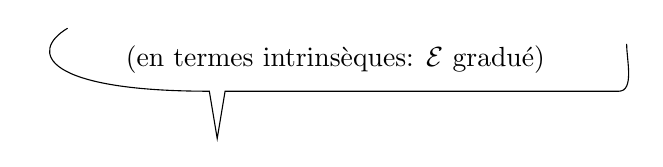
\begin{tikzpicture}[x=1cm,y=1cm]
\node at (0,.3) {(en termes intrinsèques: $\mathcal E$ gradué)};
\draw (-3.4,.7) .. controls (-3.9,.4) and (-3.7,-.1) .. (-1.6,-.1) -- (-1.5,-.7) -- (-1.4,-.1) -- (3.6,-.1) .. controls (3.8,-.1) and (3.7,.3) .. (3.7,.5);
\end{tikzpicture}}}} la seule famille d'éléments de $\mathcal E$ satisfaisant $(1.1.)$ et $(1.3)$ (a) ou b), au choix...., ou encore $(1.4)$....).

\deleted{(vi) L'élément $\Lambda$ de $\mathcal E^{(-2)}$ est uniquement déterminé, \deleted{\unsure{par les}} (en termes de \inserted{l'anneau gradué} $\mathcal E^*$ et l'élt $L\in\mathcal E^{(\unsure{1|2})}$, par les conditions suivantes :
\[
\left\{\begin{aligned}
L\Lambda&=1-\sum_{0\leq i\leq n}\pi_{i,0}\\
\Lambda L&=1-\sum_{n\leq i\leq2n}\pi_{i,0}
\end{aligned}\right.
\tag{\unsure{6.7}}
\]}

\uline{Dém.} L'équivalence de (i) et (ii) est claire, et le fait que i est impliqué par (iii) (en prenant $w_i=\Lambda^{(\unsure{n-i})}$). \deleted{\unsure{Il}}\inserted{Reste à} prouver que (i), (ii) impliquent (iii) à (vi). On \deleted{sait déjà}\inserted{\unsure{a déjà dit|a déjà dit que}} que ça implique \deleted{$(\unsure{6.7})$} (v).
\mspage{9}

\scanpage{11}
\mspage{8}
Prouvons (iv). Supposons prouvé
\[
\pi_{j\alpha}\in\mathcal E\quad\text{pour}\quad j\notin[i,2n-i]
\tag{6.7}
\]
où $i\leq n$, et prouvons que
\deleted{\[\pi_{j\alpha}\in\mathcal E\quad\text{pour}\quad j\unsure{\in}\]}
\[
\pi_{j\alpha}\in\mathcal E\quad\text{pour }j=i\text{ ou }j=2n-i,
\tag{6.7'}
\]
ce qui prouvera (iv) \inserted{\figure{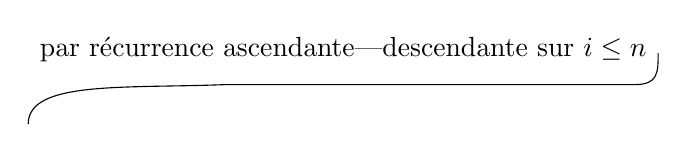
\begin{tikzpicture}[x=1cm,y=1cm]
\node at (0,.25) {par récurrence \unsure{ascendante|descendante} sur $i\leq n$};
\draw (-4,-.7) .. controls (-4,-.15) and (-2.8,-.25) .. (-1.5,-.2) -- (3.7,-.2) .. controls (4,-.2) and (4,-.05) .. (4,.2);
\end{tikzpicture}}}. Pour prouver $6.8.$ on procède par récurrence \deleted{\unsure{sur}} descendante sur $\alpha$, en supposant que
\[
\deleted{\unsure{\pi_{j\alpha}}}\quad\pi_{i,\alpha'}\in\mathcal E,\quad\pi_{2n-i,\alpha'}\in\mathcal E\quad\text{si }\alpha'>\alpha,
\tag{6.8}
\]
et on en conclura que
\[
\pi_{i,\alpha}\in\mathcal E,\quad\pi_{2n-i,\alpha}\in\mathcal E.
\tag{6.8'}
\]
\deleted{\unsure{Car|Cela} \deleted{doit} prouvera bien $(6.7')$, puisque on peut démarrer la récurrence ($\pi_{i,\alpha}=\pi_{2n-i,\alpha}=0$ si $\alpha$ grand). Si $\alpha=0$, on gagne grâce à la relation
\[
\sum_\alpha\pi_{i,\alpha}=\pi_i\quad\text{donc}\quad\pi_{i,0}=\pi_i-\sum_{\alpha\geq1}\pi_{i\alpha},
\tag{6.9}
\]
donc il suffit d'envisager le cas $\alpha\geq1$.}

Posons
\[
q_{i,\alpha}=1-\sum_{\alpha'>\alpha}\pi_{i,\alpha'}=\sum_{\alpha'\leq\alpha}\pi_{i,\unsure{\alpha|\alpha'}}
\]
donc grâce à $(6.8)$ on a
\[
q_{i,\alpha}\in\mathcal E\quad\deleted{\unsure{\mathcal E}}
\]
\mspage{10}

\scanpage{12}
\mspage{9}
Alors on voit que
\[
L^{n-i+\alpha}q_{i\alpha}:M^i\unsure{-|\longrightarrow}M^{2n-i+2\alpha}
\]
est nul sur les $L^{\alpha'}P^{i-2\alpha'}$ pour $\alpha'\neq\alpha$, et que sur $L^\alpha P^{i-2\alpha}$, \deleted{\unsure{il}} son composé avec
\[
P^{i-2\alpha}\xrightarrow{L^\alpha}L^\alpha P^{i-2\alpha}
\]
n'est autre que l'isom
\[
L^{\unsure{n-i-2\alpha|n-i+2\alpha}}:P^{i-2\alpha}\unsure{\Rightarrow|\longrightarrow}L^{n-i+2\alpha}P^{i-2\alpha}\subset M^{2n-i+2\alpha}.
\]
Il s'ensuit aussitôt que
\[
\pi_{i,\alpha}=L^\alpha w_{i-2\alpha}L^{n-i+\alpha}q_{i\alpha}=L^\alpha w_{i-2\alpha}L^{n-i+\alpha}(1-\sum_{\alpha'>\alpha}\pi_{i,\unsure{\alpha'}}
\tag{6.9}
\]
ce qui donne bien $\pi_{i\alpha}\in\mathcal E$. \deleted{Cela prouve (iv).}
Si $i<n$, il faut, \unsure{égalt} $\pi_{2n-i,\alpha}\in\mathcal E$. On
\deleted{Reste à prouver \inserted{(iii)} $\Lambda\in\mathcal E$. Il suffit de \deleted{\unsure{prendre}} \unsure{poser}
\[
q_{2n-i,\alpha}=1-\sum_{\alpha'>\alpha}\pi_{2n-i,\alpha'}
\]
et on voit alors que
\[
\deleted{\unsure{L^{n-i+\alpha}}}L^\alpha q_{2n-i,\alpha}:M^{2n-i}\unsure{-|\longrightarrow}M^{2n-i+2\alpha}
\]}
le déduit p. ex. de la formule
\[
\pi_{2n-i,\alpha}=L^{n-i}\pi_{i,\alpha}w_i\deleted{\unsure{\pi_{2n-i}}}
\tag{6.10}
\]
Cela prouve \inserted{\figure{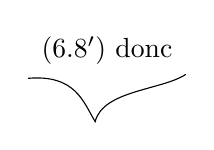
\begin{tikzpicture}[x=1cm,y=1cm]
\node at (0,.25) {$(6.8')$ donc};
\draw (-1,-.1) .. controls (-.4,-.05) and (-.3,-.4) .. (-.15,-.65) .. controls (-.05,-.25) and (.7,-.25) .. (1,-.05);
\end{tikzpicture}}} (iv). Reste : prouver (iii) $\Lambda\in\mathcal E$.

Comme on a
\[
\Lambda=\sum_{j,\alpha\,\deleted{\unsure{j\leq n}}}\deleted{\unsure{\Lambda}}\Lambda\pi_{j,\alpha}\quad\deleted{\unsure{+\sum_{0\leq i\leq n}\pi_{i,0}\Lambda}}
\tag{6.11}
\]
il suffit de prouver que $\Lambda\pi_{i\alpha}\deleted{\unsure{\Lambda\pi_{i,\alpha}|\pi_{i,\alpha}}}\in\mathcal E$.
\mspage{11}

\scanpage{13}
\mspage{10}
Or si $i\leq n$, on aura
\[
\left\{\quad\Lambda\pi_{i0}=0,\qquad\Lambda\pi_{i\alpha}=L^{\unsure{\alpha-1}}w_{i-2\alpha}L^{n-i+\alpha}\pi_{i\alpha}\quad\text{si }\alpha\geq1,\right.
\tag{6.12}
\]
\deleted{et si $j>n$, on aura
\[
\Lambda\pi_{j\alpha}=L
\tag{6.12}
\]}
\[
\Lambda\pi_{2n-i,\alpha}=L^{n-i+\unsure{\alpha}-1}w_{i-2\alpha}\deleted{\unsure{\pi_{2n-i,\alpha}}}L^\alpha\pi_{2n-i,\alpha}\quad(\text{si }i\unsure{\leq|<}n-1)
\tag{6.13}
\]
\margin{Les conditions envisagées impliquent évidemment (iv) : prouver que (iv) implique (ii). Il suffit de prouver en fait que l'on a alors $\pi_i=\pi'_i$. \uline{Démonstration à fournir.}}

\uline{Remarque} Voici un système de conditions déterminant de façon unique les éléments $\Lambda\in\mathcal E^{\unsure{(2)|(-2)}},\ \pi_{i,\alpha}\in\mathcal E^{(0)}$ en termes de $L$, et des $\pi_i\deleted{\unsure{\alpha}}$ (dont nous avons déjà une caractérisation intrinsèque par ailleurs, en termes de l'anneau gradué $\mathcal E$) :
\margin{\deleted{$\unsure{\pi_{2n-i}}$}}
\[
\left\{\begin{aligned}
\textcircled{1}\quad &(\Lambda^{n-i}L^{n-i}-1)\pi_i=0
\qquad\textcircled{2}\quad\deleted{\unsure{\pi_{2n-i}}}(L^{n-i}\Lambda^{n-i}-1)\deleted{\unsure{\pi_{2n-i}}}\pi_{2n-i}=0\\
\textcircled{3}\quad &\pi_{i,\alpha}=L^\alpha\deleted{\unsure{w_{i-2\alpha}}}\inserted{\Lambda^{n-i+2\alpha}}L^{n-i+\alpha}\bigl(1-\sum_{\alpha'>\alpha}\pi_{i,\alpha'}\bigr)\\
\textcircled{4}\quad &\pi_{2n-i,\alpha}=L^{n-i}\pi_{i,\alpha}\Lambda^{n-i}\\
&\deleted{\Lambda=\sum_{j,\alpha}\Lambda\pi_{j\alpha}}\\
\textcircled{5}\quad &\Lambda\pi_{i,0}=0\qquad\deleted{\unsure{\alpha}}\\
\textcircled{6}\quad &\Lambda\pi_{i\alpha}=L^{\alpha-1}\Lambda^{n-i+2\alpha}L^{n-i+\alpha}\pi_{i\alpha}\quad\text{si }\alpha\geq1\\
\textcircled{7}\quad &\Lambda\pi_{2n-i,\alpha}=L^{n-i+\alpha-1}\Lambda^{n-i+2\alpha}L^\alpha\pi_{2n-i,\alpha}\quad\text{si }\unsure{\alpha|i}\leq n-1\\
\textcircled{8}\quad &\Lambda=\sum_{j,\alpha}\Lambda\pi_{j\alpha}
\end{aligned}\right.
\tag{6.14}
\]
(dans ttes ces formules, on suppose $i\leq n$).

Dans ces huit formules, on peut d'ailleurs remplacer les quatre dernières par les suivantes \inserted{\figure{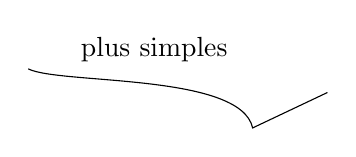
\begin{tikzpicture}[x=1cm,y=1cm]
\node at (0,.35) {plus simples};
\draw (-1.6,.1) .. controls (-1.2,-.1) and (1.1,.05) .. (1.25,-.65) -- (2.2,-.2);
\end{tikzpicture}}} :
\mspage{12}

\scanpage{14}
\figure{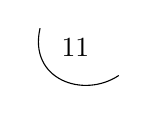
\begin{tikzpicture}[x=1cm,y=1cm]
\node at (0,0) {\mspage{11}};
\draw (-.45,.25) .. controls (-.6,-.4) and (.1,-.65) .. (.55,-.35);
\end{tikzpicture}}
\[
\left\{\begin{aligned}
L\Lambda&=1-\sum_{0\leq i\leq n}\pi_{i,0}\\
\Lambda L&=1-\sum_{n\leq j\leq2n}\pi_{\deleted{\unsure{2}}j,0}
\end{aligned}\right.
\tag{6.15}
\]
\deleted{Quant aux $\pi_{j,0}$, ils sont déterminés par les}

\uline{Question} Donner un système de \deleted{\unsure{générateurs}} relations entre les $\Lambda,L$ exclusivement, \deleted{\unsure{et}} \unsure{de|des} relations exprimant les $\pi_i$ comme polynômes en $L,\Lambda$ .... --- qui définissent $\Lambda$ en termes de $L$ et des $\pi_i$ ....
\margin{\figure{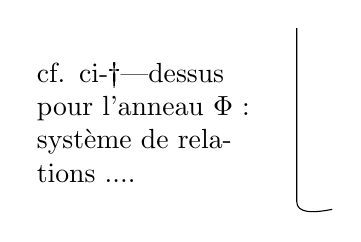
\begin{tikzpicture}[x=1cm,y=1cm]
\node[align=left,text width=3cm] at (0,0) {cf. ci-\unsure{†|dessus}\\pour l'anneau $\Phi$ :\\système de relations ....};
\draw (1.8,1.2) -- (1.8,-1) .. controls (1.8,-1.15) and (2,-1.15) .. (2.25,-1.1);
\end{tikzpicture}}}

7. Revenant à un anneau gradué abstrait $\mathcal E$, muni d'un
\[
L\in\mathcal E^{(2)},
\]
on veut abstraire la situation qui précède, sans utiliser $M^*$, en termes des propriétés du seul anneau \deleted{$\unsure{\mathcal E}$} gradué $\mathcal E^*$ muni de $L\in\mathcal E^{(2)}$.
Partons pour ceci \deleted{de} d'un module libre $\mathbf M_0$ de rang $2n$ sur $\mathbb Z$, muni d'une $2$-forme alternée non dégénérée \inserted{\figure{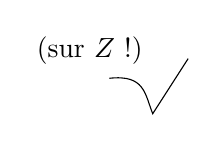
\begin{tikzpicture}[x=1cm,y=1cm]
\node at (0,.25) {(sur $\mathbb Z$ !)};
\draw (.25,-.1) .. controls (.7,-.05) and (.7,-.3) .. (.8,-.55) -- (1.25,.15);
\end{tikzpicture}}} $\xi_0\in\bigwedge^2\mathbf M_0$, \inserted{\figure{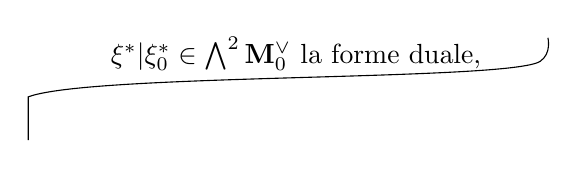
\begin{tikzpicture}[x=1cm,y=1cm]
\node at (0,.3) {$\unsure{\xi^*|\xi_0^*}\in\bigwedge^2\mathbf M_0^\vee$ la forme duale,};
\draw (-3.4,-.8) -- (-3.4,-.25) .. controls (-2.6,.05) and (2.7,-.05) .. (3.1,.2) .. controls (3.25,.3) and (3.2,.5) .. (3.2,.5);
\end{tikzpicture}}} soit \deleted{$\unsure{\xi}$} $\mathbf M_0^*=\bigwedge\mathbf M_0$, et considérons sur $\mathbf M_0^*$ les opérateurs
\[
\unsure{\mathbf L|\mathbf L_0}x=\xi_0x,\qquad\boldsymbol\Lambda_0x=\xi_0^*\mathbin{\lrcorner}x
\]
et considérons l'algèbre
\[
\Phi_0=\mathbb Z[\mathbf L_0,\boldsymbol\Lambda_0]\subset\operatorname{End}_{\mathbb Z}(\mathbf M_0^*)
\]
\margin{anneau gradué.}
Notons que $\operatorname{End}(\mathbf M_0^*)$, \inserted{\figure{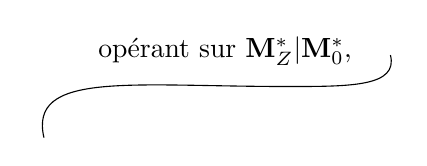
\begin{tikzpicture}[x=1cm,y=1cm]
\node at (0,.35) {opérant sur $\unsure{\mathbf M_{\mathbb Z}^*|\mathbf M_0^*}$,};
\draw (-2.3,-.75) .. controls (-2.5,.1) and (-1.2,-.1) .. (.8,-.1) .. controls (1.6,-.1) and (2.2,-.1) .. (2.1,.3);
\end{tikzpicture}}} muni de $\unsure{\mathbf L|\mathbf L_0}$, satisfait à la condition de $(6.1)\unsure{(i)|_i}$, \deleted{\unsure{donc}} et \deleted{$\unsure{\xi}$} $\boldsymbol\Lambda_0$ est l'opérateur associé défini par $(6.5)$.
\mspage{13}

\scanpage{15}
\figure{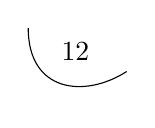
\begin{tikzpicture}[x=1cm,y=1cm]
\node at (0,0) {\mspage{12}};
\draw (-.6,.3) .. controls (-.6,-.5) and (.1,-.6) .. (.65,-.25);
\end{tikzpicture}}
\deleted{\unsure{Donc le}} $\Phi_0$ est un module libre sur $\mathbb Z$, engendré par les
\[
\varphi_i^{\beta,\alpha}\quad\deleted{\unsure{\pi_{i\alpha}}}\qquad 0\leq i\leq n,\quad0\leq\alpha,\beta\leq2n-i
\]
\deleted{\[
\left\{\quad\unsure{L^j|L^\beta}\pi_{i,\alpha}\quad\varphi_{i,\alpha}^{j,\beta}\quad\unsure{\pi_{i\alpha}}\quad\text{pour}\quad
\left\{\begin{aligned}
\unsure{i,j}\quad0\leq i\leq2n,\ 0\leq j\leq2n,\ \alpha,\beta\geq0\\
i-2\alpha=j-2\beta\geq0\\
\unsure{i<j}
\end{aligned}\right.\right.
\]}
\margin{$\mathbb Z$ \unsure{peut} être remplacé par n'importe quel anneau}
\deleted{$\varphi_{i,\alpha}^{j,\beta}$ est nul sur les composantes}
définis par
\inserted{\[
\left|\begin{aligned}
\varphi_i^{\beta\alpha}&=L_0^{\beta-\alpha}\pi_{i+2\alpha,\alpha}\quad\text{si }\alpha\leq\beta\\
\varphi_i^{\beta\alpha}&=\Lambda_0^{\alpha-\beta}\pi_{i+2\alpha,\alpha}\quad\text{si }\alpha\geq\beta\quad\deleted{\unsure{\beta-\alpha|\beta\leq\alpha}}
\end{aligned}\right.
\]}
\deleted{\[
\left\{\begin{aligned}
\varphi_{i,\alpha}^{j,\beta}&=L_0^{\beta-\alpha}\pi_{i,\alpha}=\pi_{j,\beta}L_0^{\beta-\alpha}\quad\text{si }\alpha\leq\beta\\
\varphi_{i,\alpha}^{j,\beta}&=\Lambda_0^{\alpha-\beta}\pi_{i,\alpha}=\pi_{j,\beta}\Lambda_0^{\alpha-\beta}\quad\text{si }\alpha\geq\beta
\end{aligned}\right.
\]}
i.e. on a une base formée des
\deleted{\[
\left\{L^\beta\pi_{i,\alpha}\quad\left\{\begin{aligned}
0\leq i\leq\unsure{2n|n},\quad\alpha\geq0\quad\text{donc }i-2\alpha\geq0\\
0\leq2\alpha\leq i\\
0\leq\beta
\end{aligned}\right.\right.
\]}
\margin{\[
\varphi_{i'}^{\beta',\alpha'}\varphi_i^{\beta,\alpha}\unsure{=}\left\{\begin{array}{ll}
0&\text{si }\deleted{\unsure{i-2\alpha\neq j-2\beta}}\inserted{i\neq i'\text{ ou }\beta\neq\alpha'}\\
\varphi_i^{\beta',\alpha}\deleted{\unsure{\alpha'}}&\text{sinon}
\end{array}\right.
\]
\deleted{$\unsure{\varphi_{i,\alpha}^{j,\beta}\varphi_{i',\alpha'}^{j',\beta'}=}$}}
\margin{\figure{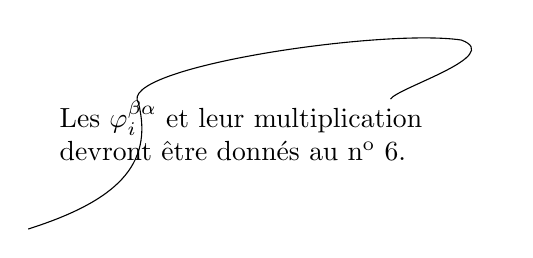
\begin{tikzpicture}
\node[align=left,text width=4.8cm,inner sep=8pt] (a) at (0,0) {Les $\varphi_i^{\beta\alpha}$ et leur multiplication \unsure{devront} être donnés au n\textsuperscript{o} 6.};
\draw (-2.8,-1.25) .. controls (-1.7,-.9) and (-1.2,-.45) .. (-1.4,.35) .. controls (-1.7,.8) and (1.7,1.3) .. (2.7,1.15) .. controls (3.25,.95) and (1.9,.55) .. (1.8,.4);
\end{tikzpicture}}}

La multiplication des bases \unsure{ne} bien sûr dépend pas du choix de $\mathbf M_0,\xi_0$ (\unsure{qui au fond} \unsure{unique est} sur l'anneau $\mathbb Z$ ....), donc l'anneau $\Phi_0$ est bien déterminé en termes de l'entier \inserted{\figure{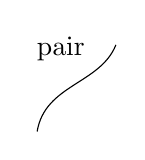
\begin{tikzpicture}[x=1cm,y=1cm]
\node at (0,.35) {pair};
\draw (-.3,-.7) .. controls (-.2,-.1) and (.5,-.1) .. (.7,.4);
\end{tikzpicture}}} $2n$.

\uline{Proposition} Revenant à la donnée de $M^*$ comme au n\textsuperscript{o} 6, et de $\mathcal E$ \deleted{\unsure{sous-algèbre}}\inserted{anneau} gradué de \deleted{$\unsure{\mathcal E}$} $\operatorname{End}(M^*)$.
\inserted{Soit $L\in\mathcal E^{(2)}$}
Conditions équivalentes

(i) L'\unsure{endom} $L$ de $M^*$ satisfait la condition de \deleted{Hard} Lefschetz et l'opérateur $\Lambda$ associé est dans $\mathcal E$.
(c. à d. on est dans les conditions du th. du n\textsuperscript{o} 6).

\unsure{(iii)|(ii)} Il existe un hom d'anneaux gradués
\[
\varphi:\Phi_0\longrightarrow\mathcal E
\]
\mspage{14}

\scanpage{16}
\figure{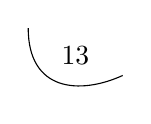
\begin{tikzpicture}[x=1cm,y=1cm]
\node at (0,0) {\mspage{13}};
\draw (-.6,.35) .. controls (-.6,-.45) and (.05,-.5) .. (.6,-.25);
\end{tikzpicture}}
appliquant $\mathbf L_0$ sur $L$, \inserted{et les $\boldsymbol\pi_i$ en les $\pi_i$ \deleted{$\unsure{\pi_i}$} (donc $\pi_i\in\mathcal E$)}.
\deleted{\unsure{respectant la graduation de} $\mathcal E$ \unsure{par les} $\pi_i$}.
\margin{\figure{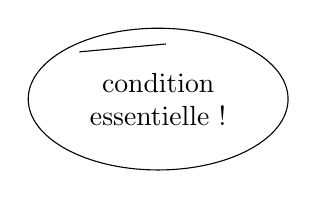
\begin{tikzpicture}
\node[align=center] at (0,0) {condition\\essentielle !};
\draw (0,0) ellipse (1.65cm and .9cm);
\draw (-1,.6)--(.1,.7);
\end{tikzpicture}}}

De plus, sous ces conditions, l'hom. annoncé \deleted{\unsure{quelque}} dans (ii) est unique, et avec les notations du n\textsuperscript{o} 6, il transforme $\boldsymbol\Lambda_0$ en $\Lambda$, les \deleted{$\unsure{\pi_{i\alpha}}$} $\boldsymbol\pi_{i\alpha}$ en $\pi_{i\alpha}$, $\boldsymbol\pi_i$ en $\pi_i$, $\boldsymbol\varphi_i^{\beta,\alpha}$ en $\varphi_i^{\beta,\alpha}$ \deleted{$\unsure{\varphi_{i,\alpha}^{j,\beta}}$}.
\margin{\figure{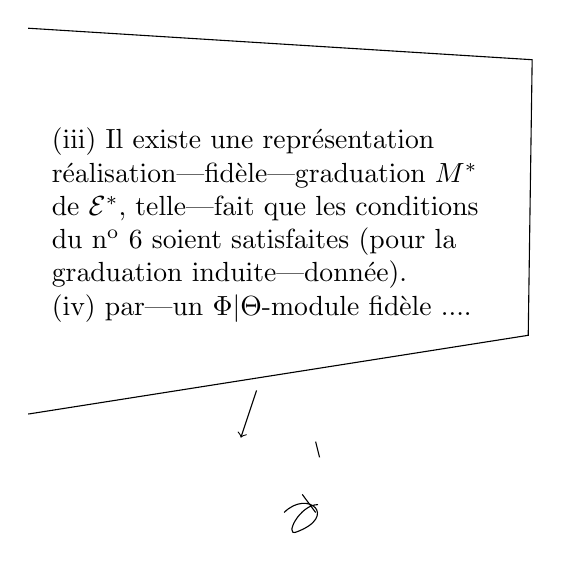
\begin{tikzpicture}
\node[align=left,text width=5.8cm] at (0,0) {(iii) Il existe une \deleted{\unsure{représentation}} \uline{\unsure{réalisation|fidèle|graduation}} $M^*$ de $\mathcal E^*$, \unsure{telle|fait} que les conditions du n\textsuperscript{o} 6 soient satisfaites (pour la graduation \unsure{induite|donnée}).\\(iv) \unsure{par|un} $\uline{\unsure{\Phi|\Theta}}$-module fidèle ....};
\draw (-3.2,2.5)--(3.2,2.1)--(3.15,-1.4)--(-3.2,-2.4);
\draw[->] (-.3,-2.1)--(-.5,-2.7);
\draw (.45,-2.75)--(.5,-2.95);
\draw (.05,-3.65) .. controls (.35,-3.35) and (.75,-3.7) .. (.2,-3.9) .. controls (.05,-3.95) and (.25,-3.55) .. (.48,-3.55);
\draw (.28,-3.42)--(.45,-3.65);
\end{tikzpicture}}}

\uline{Dém} $(i)\Rightarrow(ii)$ Résulte de la table de multiplication des $\varphi_i^{\beta,\alpha}$ donnée au n\textsuperscript{o} 6, et du th. donné au n\textsuperscript{o} 6.

$(ii)\Rightarrow(i)$ \deleted{Soient $\pi'_i$ les images des $\boldsymbol\pi_i$. On a
\[
\text{\unsure{avec}}\qquad L^\alpha\pi'_i=\pi'_{i+\alpha}L^\alpha
\]
\unsure{voit donc} que les $\pi'_i$ définissent la graduation de $\mathcal E$, parce que ils sont de degré $\unsure{0}$.
Je dis que $\pi'_i=\pi_i$ pour tt $i$. Cf Proposition ci-dessous pour ce point, appliquée à $\Phi\longrightarrow\operatorname{End}(M^*)$.}

Comme on a, pour tt $i\leq n$
\[
(\boldsymbol\Lambda_0^{n-i}\mathbf L_0^{n-i}-1)\boldsymbol\pi_i=0,\qquad
(\mathbf L_0^{n-i}\boldsymbol\Lambda_0^{n-i}-1)\boldsymbol\pi_{2n-i}=0
\]
on en conclut, appliquant $\varphi$ (et posant $\Lambda'=\varphi(\unsure{\boldsymbol\Lambda|\boldsymbol\Lambda_0})$)
\[
(\Lambda'^{n-i}L^{n-i}-1)\pi_i=0,\qquad(L^{n-i}\Lambda'^{n-i}-1)\pi_{2n-i}=0.
\]
Donc la condition (ii) du th. du n\textsuperscript{o} 6 est vérifiée, donc aussi la condition (i).

Pour l'unicité de $\varphi$, \deleted{\unsure{et les propriétés}}\inserted{il suffit} \deleted{\unsure{et les relations}} de voir que $\varphi(\unsure{\boldsymbol\Lambda|\boldsymbol\Lambda_0})=\Lambda$, et \inserted{\unsure{pour} $\varphi(\boldsymbol\pi_{i,\alpha})=\pi_{i,\alpha}$,} \deleted{\unsure{pour ceci}} \deleted{\unsure{Pour} $\varphi(\unsure{\boldsymbol\Lambda})$} compte tenu de $\varphi(\boldsymbol\pi_i)=\pi_i$, \deleted{\unsure{donc on a}} la caractérisation \inserted{\figure{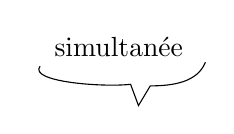
\begin{tikzpicture}[x=1cm,y=1cm]
\node at (0,.4) {simultanée};
\draw (-1,.15) .. controls (-1.15,-.05) and (-.2,-.12) .. (.15,-.08) --(.25,-.35)--(.4,-.1) .. controls (.7,-.1) and (1.0,-.05) .. (1.1,.2);
\end{tikzpicture}}} de $\Lambda$ \inserted{\figure{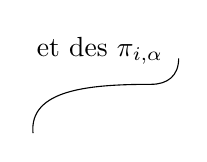
\begin{tikzpicture}[x=1cm,y=1cm]
\node at (.05,.45) {et des $\pi_{i,\alpha}$};
\draw (-.8,-.6) .. controls (-.85,-.05) and (-.1,.02) .. (.7,.02) .. controls (.9,.02) and (1.05,.12) .. (1.05,.35);
\end{tikzpicture}}} par les formules $(\unsure{6.14})$.
\mspage{15}

\scanpage{17}
\figure{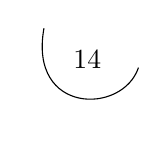
\begin{tikzpicture}[x=1cm,y=1cm]
\node at (0,0) {\mspage{14}};
\draw (-.55,.4) .. controls (-.75,-.7) and (.45,-.7) .. (.65,-.1);
\end{tikzpicture}}
\uline{Cor} Soit $\mathcal E$ un anneau gradué, \inserted{\figure{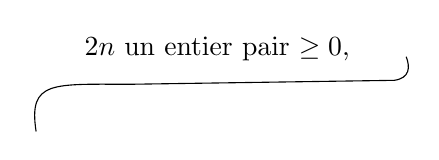
\begin{tikzpicture}[x=1cm,y=1cm]
\node at (0,.35) {$2n$ un entier pair $\geq0$,};
\draw (-2.3,-.7) .. controls (-2.4,-.05) and (-2.1,-.1) .. (-1.1,-.1) --(2.25,-.05) .. controls (2.45,-.02) and (2.45,.12) .. (2.4,.25);
\end{tikzpicture}}} et soit $L\in\mathcal E^{(2)}$.
S'il existe un hom d'anneaux gradués
\[
u:\Phi\longrightarrow\mathcal E
\]
tel que $u(\mathbf L)=L$, et tel que les $u(\boldsymbol\pi_i)=\pi_i$ définissent la graduation de $\mathcal E$ par $(1.3)$, alors un tel $u$ est uniquement déterminé, et les $\pi_i$ sont déterminés de façon unique, en termes de la structure \inserted{\uline{d'anneau}} graduée de $\mathcal E$ par les conditions $(1.1)$ et $(1.3)$.
\inserted{Si on se donne $\pi_i$ satisfaisant les conditions \deleted{\unsure{En l'absence des} $\pi_i$},}
\margin{\figure{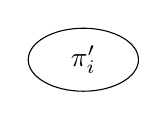
\begin{tikzpicture}\node at (0,0) {$\unsure{\pi'_i}$};\draw (0,0) ellipse (.7cm and .4cm);\end{tikzpicture}}}
l'existence de $u$ équivaut alors à \deleted{\unsure{l'existence}} la vérification, pour tt $0\leq i\leq n$, de la condition
\[
\text{``}\ \exists w_i\in\mathcal E^{-(2n-2i)}\text{ tel que}\quad(w_iL^{n-i}-1)\pi_{\deleted{\unsure{i}}\inserted{2n-i}}\deleted{=0}\text{''}=0,
\]
et \deleted{\unsure{alors}} le système des $\Lambda=u(\boldsymbol\Lambda)$, \deleted{et} $\pi_{i,\alpha}=u(\boldsymbol\pi_{i,\alpha})$ est alors caractérisé (en termes de $L$ et des $\pi_i$) par les équations $(6.14)$.
\margin{On a aussi : $\exists$ un module fidèle $M^*$ sous $\mathcal E^*$ tel que \unsure{par sa graduation} \unsure{coïncide avec} $\unsure{\pi_i}$ .... (\unsure{donc ceci pour tt i}). \deleted{\unsure{Si on dit}} \unsure{Tout précédent}.}
De la donnée des $\pi_i$, l'existence de $u$ équivaut à l'existence d'un module \uline{gradué} fidèle sous $\mathcal E^*$, \deleted{tel que} \unsure{$\mathcal E^*$} (\unsure{définie par les} $\pi_i\in\operatorname{End}(M^*)$), et tel que \figure{\begin{tikzpicture}[x=.35cm,y=.35cm,baseline]
\fill (0,0) ellipse (.09 and .045);
\fill (.5,.06) ellipse (.065 and .05);
\fill (.8,.07) ellipse (.07 and .045);
\fill (1.15,.12) ellipse (.09 and .04);
\fill (1.5,.15) ellipse (.055 and .05);
\draw[line width=.8pt] (1.9,.17) .. controls (2.05,.23) and (2.08,.23) .. (2.2,.18);
\draw[line width=.8pt] (2.5,.2)--(2.8,.21);
\fill (4.4,.22) circle (.13);
\end{tikzpicture}}

\uline{Question} Si on ne se donne \uline{pas} la graduation de $\mathcal E$ :
\inserted{\figure{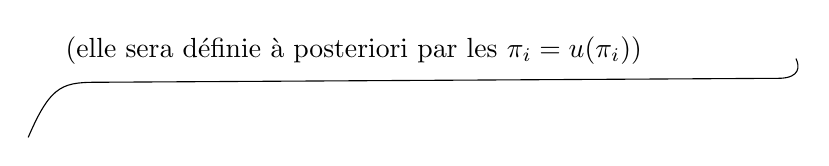
\begin{tikzpicture}[x=1cm,y=1cm]
\node[anchor=west] at (0,.35) {(elle sera définie à posteriori par les $\pi_i=u(\boldsymbol\pi_i)$)};
\draw (-.35,-.75) .. controls (-.05,-.05) and (.1,-.05) .. (.6,-.05) --(9.2,.0) .. controls (9.45,.01) and (9.45,.15) .. (9.4,.25);
\end{tikzpicture}}}
\unsure{pourrait-il|serait-il} vrai qu'il y a au plus un hom $\Phi\longrightarrow\mathcal E$ tel que $u(\mathbf L)=L$ !

\figure{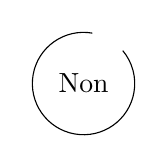
\begin{tikzpicture}\node at (0,0) {Non};\draw (80:.65cm) arc[start angle=80,end angle=400,radius=.65cm];\end{tikzpicture}}, déjà dans le cas $n=1$, $2n=2$, où il y a une base de $\Phi$ formée de $\pi_0,\pi_1,\pi_2,L,\Lambda$, et où $\mathbb Z[L]$ n'est que $\mathbb Z+\mathbb ZL$ ! Il faut donc se donner en même temps \uline{$L$ et les $\pi_i$}.
\mspage{16}

\scanpage{18}
8) Soit maintenant $\mathcal E^*$ un anneau gradué, \deleted{muni de} tel qu'il existe $L\in\mathcal E^{(2)}$ satisfaisant aux \uline{conditions de Lefschetz} (\deleted{de} les conditions du corollaire du n\textsuperscript{o} précédent). On dit que $\mathcal E^*$ est un ``anneau \deleted{d'opérateurs Lefschetzien,}\inserted{de correspondances Lefschetzien}'' (\unsure{cette} \deleted{\illegible{3}} \deleted{\unsure{avec le système}} \unsure{au n\textsuperscript{o}} \unsure{(pair)} \unsure{qu'un système de|qui un système de} Lefschetz), et $L$ un de ses ``éléments de Lefschetz''.
\deleted{\unsure{En dehors} $(\unsure{\varphi(\Phi)=\mathcal E^*})$}
L'élt $\Lambda$ associé est \deleted{\unsure{dit}} \unsure{``}l'élément \deleted{\unsure{adjoint pour}} \deleted{\unsure{anti}}\inserted{co.}Lefschetzien'' associé à $L$.
(NB. À noter que $L$ se déduit de $\Lambda$ comme $\Lambda$ de $L$, par simple symétrie sur les degrés de $\mathcal E^*$ \deleted{$\unsure{\xi_0}$} $\unsure{-}$, et passage à l'anneau opposé --- \deleted{\unsure{transposé}} isom de transposition ---).
\margin{\figure{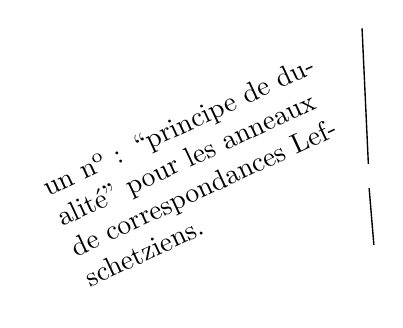
\begin{tikzpicture}
\node[align=left,text width=3.8cm,rotate=25] at (0,0) {un n\textsuperscript{o} : ``principe de dualité'' pour les anneaux de correspondances Lefschetziens.};
\draw[line width=.5pt] (2.05,1.8)--(2.13,.08);
\draw[line width=.5pt] (2.14,-.23)--(2.2,-.95);
\end{tikzpicture}}}

On peut se demander de \uline{caractériser} les \deleted{les} éléments de Lefschetz $L$. Une condition nécessaire, lorsque le \unsure{nombre} $2n$ n'est pas redondant, i.e.
\[
\begin{aligned}
1)\quad&\mathcal E^{(2n)}\neq0\quad\deleted{\unsure{\{}}\quad(\Longleftrightarrow)\quad1')\ \mathcal E^{(-2n)}\neq0\quad\deleted{\unsure{\}}}\\
&(\Longleftrightarrow)\quad2)\ \pi_0,\deleted{\unsure{\pi_{2n}}}\neq0\quad\deleted{\unsure{\}}}
\end{aligned}
\]
\margin{\figure{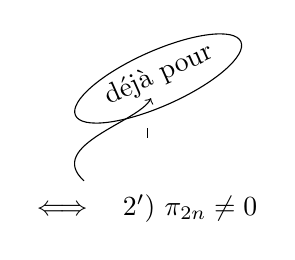
\begin{tikzpicture}
\node[align=left] at (0,0) {$\Longleftrightarrow\quad2')\ \pi_{2n}\neq0$};
\node[rotate=24] at (.15,1.7) {\unsure{déjà pour}};
\draw[rotate=24] (.8,1.45) ellipse (1.15cm and .35cm);
\draw[->] (-.8,.35) .. controls (-1.3,.8) and (-.1,1.1) .. (.05,1.4);
\draw (.01,1.02)--(.01,.9);
\end{tikzpicture}}}
que
\[
(\Longleftrightarrow)\quad3)\ L^n\neq0\quad(\Longleftrightarrow)\quad3')\ \Lambda^{\unsure{n|-}}\neq0\quad\deleted{\Longleftrightarrow}
\]
c'est que l'on ait $L^n\neq0$. On a parfois une réciproque, dans le cas où ($\mathcal E$ étant une \uline{algèbre} sur un anneau commutatif $k$)
\mspage{17}

\scanpage{19}
\mspage{45}
en groupes \deleted{localement}\figure{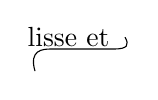
\begin{tikzpicture}[baseline=(a.base),x=1cm,y=1cm]
\node[anchor=west,inner sep=0pt] (a) at (0,0) {\inserted{lisse et}};
\draw ([xshift=.1cm,yshift=-.30cm]a.south west) .. controls ([xshift=.02cm,yshift=-.03cm]a.south west) and ([xshift=.2cm,yshift=-.02cm]a.south west) .. ([xshift=.3cm,yshift=-.02cm]a.south west) -- ([xshift=.05cm,yshift=-.02cm]a.south east) .. controls ([xshift=.22cm,yshift=-.02cm]a.south east) and ([xshift=.25cm,yshift=.03cm]a.south east) .. ([xshift=.19cm,yshift=.13cm]a.south east);
\end{tikzpicture}} de type fini sur $k$, soit $\uline{\operatorname{Pic}}_U$, et un isomorphisme
\[
\operatorname{Pic}(U)=\uline{\operatorname{Pic}}_U(k)
\tag{8.13}
\]
de $\operatorname{Pic}(U)$ avec le groupe des points à valeurs dans $k$ de $\uline{\operatorname{Pic}}_U$. Cela nous fournit donc pour $\operatorname{Pic}(U)$ une structure d'extension
\[
\diagram{\begin{tikzcd}[ampersand replacement=\&,column sep=small]
0\arrow[r]\&\operatorname{Pic}(U)^0\arrow[r]\&\operatorname{Pic}(U)\arrow[r]\&\operatorname{NS}(U)\arrow[r]\&0
\end{tikzcd}},
\tag{8.14}
\]
où on a posé
\[
\operatorname{Pic}(U)^0=\uline{\operatorname{Pic}}_U^0(k),\qquad\operatorname{NS}(U)=\uline{\operatorname{NS}}_U(k),
\tag{8.15}
\]
\deleted{\unsure{où}} $\uline{\operatorname{Pic}}_U^0$ désignant la composante neutre de $\uline{\operatorname{Pic}}_U$, et $\uline{\operatorname{NS}}_U$ le quotient de $\uline{\operatorname{Pic}}_U$ par cette composante. La construction indiquée dans loc. cit. permet d'ailleurs de préciser la structure de $\operatorname{NS}(U)$, en introduisant la matrice d'intersection
\[
(C_i.C_j)_{1\leq i,j\leq r}
\]
définie par les $r$ composantes irréductibles $C_i$ de $f^{-1}(x)_{\mathrm{r\acute ed}}$ sur le
\margin{\figure{\begin{tikzpicture}\draw (0,0)--(.18,.22);\draw (.03,.2)--(.16,.05);\end{tikzpicture}}}
schéma régulier $X'$ : en vertu de MUMFORD\figure{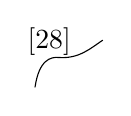
\begin{tikzpicture}[baseline=(b.base),x=1cm,y=1cm]
\node[anchor=west,inner sep=0pt] (b) at (0,0) {\inserted{[28]}};
\draw ([xshift=.10cm,yshift=-.40cm]b.south west) .. controls ([xshift=.15cm,yshift=-.05cm]b.south west) and ([xshift=.30cm,yshift=-.01cm]b.south west) .. ([xshift=.40cm,yshift=-.02cm]b.south west) .. controls ([xshift=.10cm,yshift=-.04cm]b.south east) and ([xshift=.25cm,yshift=.10cm]b.south east) .. ([xshift=.40cm,yshift=.20cm]b.south east);
\end{tikzpicture}}, cette matrice est définie négative, donc le conoyau de l'homomorphisme
\[
\uline{\mathrm Z}^{r}\longrightarrow\uline{\mathrm Z}^{r}
\]
qu'elle définit est un groupe fini, dont l'\unsure{ordre} n'est autre que la valeur absolue du déterminant de cette matrice. Ceci posé, on trouve que $\operatorname{NS}(U)$ est canoniquement isomorphe à ce groupe fini. La matrice envisagée étant symétrique, on voit aussitôt que ce groupe est canoniquement autodual (par un accouplement \deleted{\unsure{symétrique|canonique}}\inserted{\uline{symétrique}} à valeurs dans $\uline{\mathrm Q}/\uline{\mathrm Z}$), d'où une autodualité \figure{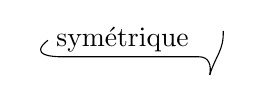
\begin{tikzpicture}[baseline=(c.base),x=1cm,y=1cm]
\node[anchor=west,inner sep=0pt] (c) at (0,0) {\inserted{symétrique}};
\draw ([xshift=-.10cm,yshift=.16cm]c.south west) .. controls ([xshift=-.35cm,yshift=-.04cm]c.south west) and ([xshift=-.03cm,yshift=-.05cm]c.south west) .. ([xshift=.08cm,yshift=-.05cm]c.south west) -- ([xshift=.12cm,yshift=-.05cm]c.south east) .. controls ([xshift=.25cm,yshift=-.05cm]c.south east) and ([xshift=.28cm,yshift=-.15cm]c.south east) .. ([xshift=.26cm,yshift=-.28cm]c.south east);
\draw ([xshift=.26cm,yshift=-.28cm]c.south east) .. controls ([xshift=.33cm,yshift=-.04cm]c.south east) and ([xshift=.44cm,yshift=.03cm]c.south east) .. ([xshift=.43cm,yshift=.28cm]c.south east);
\end{tikzpicture}}
\[
\operatorname{NS}(U)\times\operatorname{NS}(U)\longrightarrow\uline{\mathrm Q}/\uline{\mathrm Z},
\tag{8.16}
\]
dont on constate aisément qu'elle est indépendante de la résolution $X'$ choisie.

Si maintenant $\ell$ est un nombre premier distinct de $\operatorname{car}k$, alors la structure connue des groupes algébriques commutatifs connexes sur $k$ \inserted{[9, exp.4]} montre que $\operatorname{Pic}(U)_0$ est un groupe $\ell$-divisible, donc
\margin{\figure{\begin{tikzpicture}\draw (0,0)--(.18,.22);\draw (.03,.2)--(.16,.05);\end{tikzpicture}}}
\figure{\begin{tikzpicture}[x=.003cm,y=-.003cm]
\draw (535,170) .. controls (600,760) and (900,1600) .. (1100,2070);
\draw (270,840) .. controls (300,860) and (360,1600) .. (520,2080);
\draw (1235,60) .. controls (1310,270) and (1350,580) .. (1475,750);
\end{tikzpicture}}
\mspage{18}

\scanpage{20}

\deleted{$\unsure{b'}$}
\figure{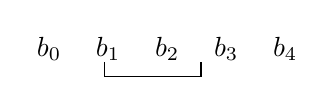
\begin{tikzpicture}
\node at(0,0){$b_0$};\node at(.75,0){$b_1$};\node at(1.5,0){$b_2$};\node at(2.25,0){$b_3$};\node at(3,0){$b_4$};
\draw(.7,-.17)--(.7,-.35)--(1.93,-.35)--(1.93,-.17);
\end{tikzpicture}}
\[
nb_0+(n-1)b_1=\qquad L
\]
\figure{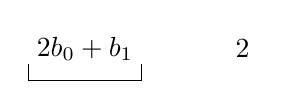
\begin{tikzpicture}
\node at(0,0){$2b_0+b_1$};\node at(2,0){$2$};
\draw(-.72,-.2)--(-.72,-.4)--(.72,-.4)--(.72,-.2);
\end{tikzpicture}}
\[
\lambda^{(n-i)b_i}\qquad\mathcal E^{n-i}\qquad
\mathcal E^{\unsure{2i|i}}\times\mathcal E^{2n-2i}
\]
\deleted{$\unsure{\lambda}$}
\diagram{\begin{tikzcd}[ampersand replacement=\&]
M^0\arrow[r]\&M^{\unsure{2n|n}}
\end{tikzcd}}
\deleted{$\Lambda\quad\lambda L\sim$}
\[
L\sim\lambda L\quad\text{\unsure{alors}}\quad\Lambda\sim\frac1\lambda\Lambda
\]
\deleted{$\unsure{\xi|\chi}$}
\[
\Lambda=P(L
\]
\[
\Lambda=\Omega(L)\Delta(L)^{-N}.
\]
\margin{\deleted{$\unsure{LL'}\quad L'^2=LL'$}}
\[
\uline{L'}\quad\uline{LL'}\quad\uline{L^2L'}\quad\deleted{L^4}\quad L^3L'
\]
\[
\left(L^4,\ L'^2-LL',\ L^2L'-L^3,\ L^3L'\right)
\]
\diagram{\begin{array}{c|c|c|c|}
1&L,L'&L^2,LL'&L^3
\end{array}}
\diagram{\begin{tikzcd}[ampersand replacement=\&,column sep=small]
H^0\arrow[rrrr,bend right=20]\&H^1\arrow[rr]\&H^2\&H^3\&H^4
\end{tikzcd}}
\[
L'^3\deleted{\unsure{L}}=L'^2L=L^2L'=L^3
\]
\diagram{\begin{tikzcd}[ampersand replacement=\&,column sep=large]
H^0\arrow[r,dash]\&H^2\arrow[r,dash]\&H^4\arrow[r,dash]\&H^6\\[-1em]
\uuline{\text{rg }1}\&\uuline{\text{rg }2}\&\uuline{\text{rg }2}\&\uuline{\text{rg }1}
\end{tikzcd}}
\[
\unsure{V}\qquad\deleted{\sum V}\qquad\operatorname{Sym}^{\unsure{2}}(V)\mathbin{-}V\mathbin{-}
\]
\[
\unsure{k|2}
\]
\[
L,L'\qquad L^2=\bar L,\quad L\bar L'=\bar L',\quad \bar L'{}^2=\unsure{\overline{\bar L'}|\bar L'}
\]
\[
L^2,L',LL'.\qquad L'
\]
\[
\begin{gathered}
L,L'\\
L^2,LL'\qquad L'^2=LL'\\
L^3=L^2L'
\end{gathered}
\qquad
L'^3=LL'^2=L^2L'
\]
\[
\mathbb Z[L]/(L^4)\deleted{\unsure{\mathbb Z}}[L']/L'^2-L^{\unsure{\prime\prime|\prime}}
\]

\mspage{19}

\scanpage{21}

\mspage{42}

on trouve une suite exacte canonique \inserted{(où $Z_\ell[1]=\varprojlim_\nu\deleted{Z}\mu_{\ell^\nu}$ est le faisceau $\ell$-adique de TATE)}:
\diagram{\begin{tikzcd}[ampersand replacement=\&,column sep=small]
(8.3)\quad0\arrow[r]\&t^{i-1}(X,\ell)\arrow[r]\&H^i(X,\uline Z_\ell[1])\arrow[r]\&T_\ell(H^i(X,\mu_{\ell^\infty}))\arrow[r]\&0,
\end{tikzcd}}
où \deleted{$\unsure{t^{i-1}(X,\ell)}$} on a posé
\[
(8.4)\qquad t^{i-1}(X,\ell)=H^{i-1}(X,\mu_{\ell^\infty})/H^{i-1}(X,\mu_{\ell^\infty})^0
\]
qui est donc un groupe fini de $\ell$-torsion, et s'identifie donc, par (8.3), au sous-\deleted{groupe}\inserted{module} de torsion de $\uline Z_\ell$-module de type fini
\[
(8.5)\qquad H^i(X,\uline Z_\ell[1])=\lim H^i(X,\mu_{\ell^\nu}\deleted{\unsure{\ell^\nu Z}}),
\]
dont la partie libre s'identifie, à son tour, à $T_\ell(H^i(X,\mu_{\ell^\infty}))$. On en déduit également un isomorphisme
\[
(8.6)\qquad \deleted{\unsure{T}}(H^i(X,\mu_{\ell^\infty})^0\simeq H^i(X,\uline Z_\ell[1])\otimes_{\uline Z_\ell}\uline Q_\ell/\operatorname{Im}H^i(X,\uline Z_\ell[1]),
\]
qui montre que $H^i(X,\mu_{\ell^\infty})$ et $H^i(X,\uline Z_\ell[1])$ se déterminent mutuellement mod groupes \deleted{\unsure{dant|d'ordre}} finis.

\inserted{8.2.} Un passage à la limite analogue dans \deleted{les suites exactes}\inserted{la suite exacte} de Kummer (BR II 3.1) nous donne de même une suite exacte
\diagram{\begin{tikzcd}[ampersand replacement=\&,column sep=small]
(8.7)\quad0\arrow[r]\&\operatorname{NS}(X)\otimes_{\uline Z}\uline Z_\ell\arrow[r]\&H^2(X,\uline Z_\ell[1])\arrow[r]\&T_\ell(\operatorname{Br}'(X))\arrow[r]\&0,
\end{tikzcd}}
en supposant maintenant que $\operatorname{Pic}(X)$ est extension d'un groupe de type fini $\operatorname{NS}(X)$ (le \uline{groupe de Néron--Sévéri}) par un groupe divisible, et que $H^2(X,\uline Z/\ell\uline Z)$ est fini. \deleted{\unsure{x}}On trouve en passant le fait, classique dans la théorie transcendante, que \deleted{le}\inserted{\figure{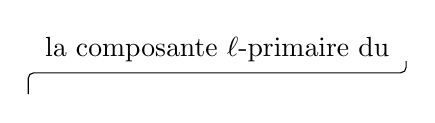
\begin{tikzpicture}
\node at(0,0){la composante $\ell$-primaire du};
\draw[rounded corners=2pt](-2.4,-.57)--(-2.4,-.3)--(2.4,-.3)--(2.4,-.15);
\end{tikzpicture}}} sous-groupe de torsion de $\operatorname{NS}(X)$ est isomorphe au sous-groupe de torsion de $H^2(X,\uline Z_\ell[1])$, en même temps qu'on précise du point de vue de la cohomologie $\ell$-adique la relation entre le groupe de Brauer (ou plus précisément, $T_\ell(\operatorname{Br}'(X))$) et la ``partie transcendante'' du $H^2$, \deleted{\unsure{x}}comparer (BR II 3 passim).

Lorsque $X$ est \inserted{\figure{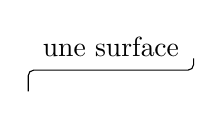
\begin{tikzpicture}
\node at(0,0){une surface};
\draw[rounded corners=2pt](-1.05,-.57)--(-1.05,-.3)--(1.05,-.3)--(1.05,-.15);
\end{tikzpicture}}} propre, lisse et connexe sur un corps $k$ algébriquement clos, il y a lieu de considérer sur le terme médian de (8.7) la forme bilinéaire symétrique canonique, fournie par le cup-produit,\deleted{\unsure{à|x}} qui est à valeurs dans

\mspage{20}

\scanpage{22}
$\mathcal E^{2n}$ \deleted{est engendré par} \inserted{admet la \uline{base}} $L_0^n$,
\inserted{(pour un $L_0$ de Lefschetz fixé)}
\deleted{$\mathcal E^{-2n}$ \unsure{engendré} par $\unsure{\Lambda_0^n|\Lambda^n}$,}
\deleted{pour un choix de $(L,\Lambda)$.}
\deleted{de $\mathcal E^{2n}$, \illegible{2} de $L'$.}
Or.\,--- où, si $L'$ est un autre élément Lefschetzien
\figure{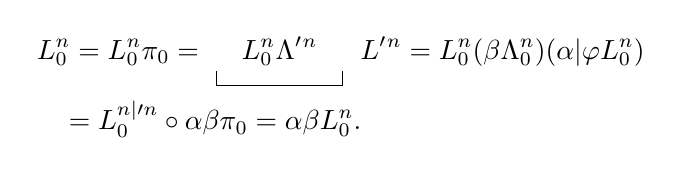
\begin{tikzpicture}
\node[anchor=base east] at(-.9,0){$\displaystyle L_0^n=L_0^n\pi_0=$};
\node[anchor=base] at(0,0){$\displaystyle L_0^n\Lambda'{}^n$};
\node[anchor=base west] at(.9,0){$\displaystyle L'{}^n=L_0^n(\beta\Lambda_0^n)(\unsure{\alpha|\varphi}L_0^n)$};
\draw(-.8,-.15)--(-.8,-.33)--(.8,-.33)--(.8,-.15);
\node[anchor=base west] at(-2.8,-.9){$\displaystyle =L_0^{\unsure{n|\prime n}}\circ\alpha\beta\pi_0=\alpha\beta L_0^n.$};
\end{tikzpicture}}
ce qui prouve que $\alpha\beta=1$, donc $\alpha$ et $\beta$ inversibles, donc \deleted{\unsure{pour}} $L_0^{\unsure{\prime n|n}}$ et $\Lambda_0^{\unsure{\prime n|n}}$ sont des bases de $\mathcal E^{(2n)}$ et $\mathcal E^{(-2n)}$ respectivement.

D'où
\diagram{\begin{tikzcd}[ampersand replacement=\&,column sep=large]
L^{\unsure{\prime|*}}\ \text{Lefschetzien}\arrow[r,Rightarrow]\&L^n\ \text{\uline{une base de}}\ \mathcal E^{2n}
\end{tikzcd}}
\figure{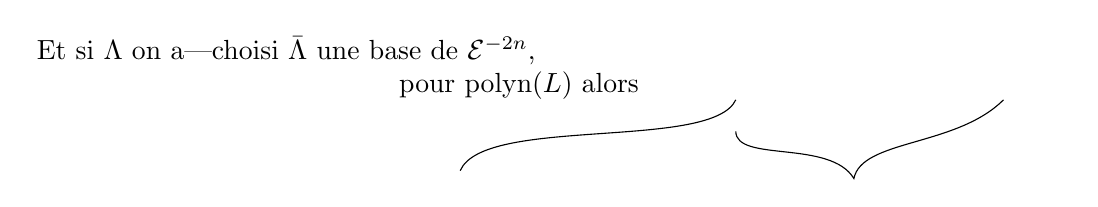
\begin{tikzpicture}[x=1cm,y=1cm]
\node[anchor=west,align=left,text width=13cm] at (0,1.1) {\inserted{Et si $\deleted{\unsure{\Lambda}}$ \unsure{on a|choisi} $\bar\Lambda$ une base de $\mathcal E^{-2n}$,\\\hspace*{4.6cm}\unsure{pour} \uline{\unsure{polyn}}$(L)$ \unsure{alors}}};
\draw (5.5,-.2) .. controls (5.8,.5) and (8.7,.05) .. (9,.7);
\draw (9,.3) .. controls (9,-.1) and (10.2,.2) .. (10.5,-.3) .. controls (10.6,.2) and (11.8,.1) .. (12.4,.7);
\end{tikzpicture}}
\margin{?}
On \unsure{veut|peut} prouver une réciproque, dans le cas où \deleted{$\unsure{\mathcal E}$} $\mathcal E$ est projectif de type fini sur $A$. \unsure{Ça|Ce} ne marche certainement pas tel quel, p.ex. pour $\mathcal E=\mathcal L(M^*)$, $M^*$ gradué à degrés $0\leq i\leq4$ ---.

Mais ça ne marche pas non plus pour les endom. associés aux élémts de degré $2$ d'une alg. de Lefschetz, pour la dim $6$

$\mathcal E$ engendré par $L,L'$ \inserted{\figure{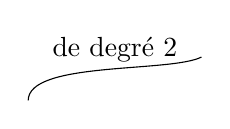
\begin{tikzpicture}
\node at(0,0){de degré $2$};
\draw(-1.1,-.65) .. controls(-1.1,-.15) and(.7,-.3) .. (1.1,-.1);
\end{tikzpicture}}} avec les relations
\[
L^4=0,\quad L'^2-LL'=0,\quad L^2L'-L^3=0,\quad L^3L'=0,\qquad\text{de base}
\]
\diagram{\begin{array}{r c||c||c||c}
&1&L,L'&L^2,LL'&L^3\\\cline{2-5}
\text{degré}&0&2&4&
\end{array}}
\margin{\figure{\begin{tikzpicture}
\draw(.3,1.5) .. controls(.25,.7) and(.1,.3) .. (0,0);
\node[anchor=west,align=left,text width=5.1cm] at(.4,.75){$L$ est Lefschetzien,\\$L'$ ne l'est pas, bien que\\$L'^3=L^3$ !};
\end{tikzpicture}}}
\mspage{21}

\scanpage{23}
\mspage{43}
\figure{\begin{tikzpicture}[x=1cm,y=1cm]
\node[anchor=west] at (.35,0) {\inserted{(en négligeant la torsion du $H^2$) est non dégénérée, et}};
\draw (0,.6) -- (0,-.35) .. controls (0,-.5) and (.15,-.5) .. (.3,-.5) -- (12.5,-.5) .. controls (12.8,-.5) and (13,-.4) .. (13,.6);
\draw (.3,-.15) circle (.055);
\draw (.3,-.1)--(.7,.5);
\end{tikzpicture}}
\[
H^4(X,\underline Z_{\ell}[2])\simeq\underline Z_{\ell}.
\]
\deleted{D'après \unsure{il est}} Cette forme\figure{\begin{tikzpicture}[baseline=-.3ex,x=.4cm,y=.4cm]\draw (0,0) circle (.07);\draw (.03,.07)--(.5,.9);\end{tikzpicture}} induit sur $\operatorname{NS}(X)\otimes_{\underline Z}\underline Z_{\ell}$ la forme bilinéaire déduite de la \uline{forme intersection} sur $\operatorname{NS}(X)$, provenant de la multiplicité
\margin{$\times$}
globale d'intersections de diviseurs sur $X$ \inserted{[15]} \deleted{\unsure{?}}. D'après
\margin{$\times$}
MATSUSAKA \inserted{[27]}, cette dernière forme est non dégénérée. Tensorisant alors la suite exacte (8.7) par $\underline Q_{\ell}$, on trouve que $T_{\ell}(\operatorname{Br}^{\deleted{\unsure{\prime}}}(X))\otimes_{\underline Z_{\ell}}\underline Q_{\ell}$ \uline{s'identifie canoniquement à l'orthogonal de} $\operatorname{NS}(X)\otimes_{\underline Z_{\ell}}\underline Q_{\ell}$ \uline{dans} $H^2(X,\underline Q_{\ell}[1])$, \uline{et que le cup-produit définit sur cet espace une forme quadratique non dégénérée.}
L'interprétant comme une forme quadratique sur $T_{\ell}(\operatorname{Br}^{\deleted{\unsure{\prime}}}(X))$ à valeurs dans $\underline Q_{\ell}$, (et tenant compte que le cup-produit induit même une autodualité de $H^2/\mathrm{torsion}$) on trouve aisément que cette forme est à valeurs dans $\underline Z_{\ell}$ si et seulement si le discriminant de la forme intersection sur $\operatorname{NS}(X)/\mathrm{torsion}$ est une unité $\ell$-adique - condition qui est vérifiée donc pour presque tous les nombre premiers $\ell$ \deleted{\unsure{-}}, et que dans ce cas on trouve une autodualité de $T_{\ell}(\operatorname{Br}^{\deleted{\unsure{\prime}}}(X))$.

\inserted{8.3.} Ce résultat ne concerne essentiellement que la partie divisible $\operatorname{Br}'(X)^0$ du groupe de Brauer cohomologique. On peut également donner une relation de dualité concernant le \deleted{\unsure{gour|grou}} groupe fini $\operatorname{Br}'(X)/\operatorname{Br}'(X)^0$, qui grâce à la suite exacte de Kummer (BR II 3.1) s'explicite comme
\[
\tag{8.8}\operatorname{Br}'(X)/\operatorname{Br}'(X)^0\simeq H^2(X,\mu_{\ell^\infty})/H^2(X,\mu_{\ell^\infty})^0,
\]
(compte tenu que $\operatorname{Pic}(X)\otimes\underline Q_{\ell}/\underline Z_{\ell}=\operatorname{NS}(X)\otimes\underline Q_{\ell}/\underline Z_{\ell}$ est divisible). Utilisant (8.3) pour $i=3$, on trouve donc
\[
\tag{8.9}\operatorname{Br}'(X)/\operatorname{Br}'(X)^0\simeq\operatorname{Tors}H^3(X,\underline Z_{\ell}[1]),
\]
\inserted{(}valable indépendamment des hypothèses particulières \deleted{\unsure{faites}} \inserted{posées} au début de l'alinéa précédent pour $X$. Lorsque celles-ci sont vérifiées, alors les relations de dualité, bien connues dans le cas classique, et qui résultent aisément \figure{\begin{tikzpicture}[baseline=(p.base),x=1cm,y=1cm]
\node[inner sep=0pt,anchor=west] (p) at (0,0) {\inserted{par passage à la limite}};
\draw ([xshift=-.08cm,yshift=-.30cm]p.south west) -- ([xshift=-.08cm,yshift=-.10cm]p.south west) .. controls ([xshift=-.08cm,yshift=-.03cm]p.south west) and ([yshift=-.02cm]p.south west) .. ([xshift=.08cm,yshift=-.02cm]p.south west) -- ([xshift=-.08cm,yshift=-.02cm]p.south east) .. controls ([xshift=.08cm,yshift=-.02cm]p.south east) and ([xshift=.10cm,yshift=.02cm]p.south east) .. ([xshift=.10cm,yshift=.12cm]p.south east);
\end{tikzpicture}} des résultats de dualité [SGAA $\overline{\underline{\mathrm{XIX}}}$\quad] pour des
\margin{$\times$}
\mspage{22}

\scanpage{25}
\begin{flushright}\fbox{Algèbres de Hodge d'ordre 2}\end{flushright}
\diagram{\begin{array}{ccccc}
H^0&H^1&H^2&H^3&H^4\\
k&V&k\xi+W&\check V&k\xi^2
\end{array}}

$V,W$

\[
\bigwedge^2 V\xrightarrow{\alpha}k\xi+W
\qquad \alpha(x\wedge y)=\varphi(x,y)\xi+\psi(x,y)
\]
\[
\operatorname{Sym}^2(W)\xrightarrow{\beta}k\xi^2
\qquad \beta(xy)=Q(x,y)\xi^2
\]
\margin{$\varphi(x,y)$ forme alternée\par
$\psi(x,y)$ -- \unsure{appl.} bil. alt. dans $W$\par
$Q$ forme bil. sym. sur $W$}

\deleted{\unsure{Point de vue}}
La connaissance de $V,W,\varphi,\psi,\unsure{Q|\bar Q}$ permet de reconstituer $H^*$ :
\unsure{isom.} canonique près.

\[
H^0\times H^i\longrightarrow H^i:\quad\text{clair par}\quad
1.x=x.1=x\qquad\forall x.
\]
\[
H^1\times H^i\longrightarrow H^{i+1}\quad
\left|\begin{array}{ll}
\deleted{\unsure{donc}}\ i=1&xy=\varphi(x,y)\xi+\psi(x,y)\qquad x,y\in V\\
i=2&\begin{array}{l}
x\xi=\xi x=\widetilde\varphi(x):\quad\deleted{\unsure{(*)}}\ y\longmapsto\varphi(y,x)\\
xw=wx=\unsure{\rho'|\rho^1}(w,x):\quad y\longmapsto Q(\psi(y,x),w)
\end{array}\quad\left|\begin{array}{l}x\in V\\y\in V\\w\in W\end{array}\right.\\
i=3&xy'=-y'x=\unsure{\langle x,y'\rangle|+\langle x,y'\rangle}\xi^2\qquad x\in V,y'\in\check V\\
\deleted{\unsure{i=4}}&\deleted{\unsure{x\xi^2=0}}
\end{array}\right.
\]
\[
H^2\times H^i\longrightarrow H^{i+2}\quad
\left|\quad i=2:\quad\left|\begin{array}{l}
\xi.\xi=\xi^2\\
\xi w=w\xi=0\quad(w\in W)\\
ww'=Q(w,w')\xi^2
\end{array}\right.\right.
\]
\figure{\begin{tikzpicture}[x=1cm,y=1cm]
\node[anchor=west,align=left] at (.2,0) {(*) On pose $\widetilde\varphi:V\longrightarrow\check V$, avec\\[.5em]$\langle x,\widetilde\varphi(y)\rangle=\varphi(x,y)$};
\draw (-2.4,.9) .. controls (-1.1,1) and (0,.9) .. (0,.5) -- (.2,-.7) .. controls (.2,-.85) and (.4,-.9) .. (.7,-.9) -- (8.9,-.9);
\end{tikzpicture}}

\unsure{Quelle que soit la donnée} de $\varphi,\psi$, on trouve une loi de composition
anticommutative, admettant $1$ comme unité.

\uline{Condition d'associativité} s'écrit $(xy)(tz)=(tx)(yz)$, sous la forme
\[
\deleted{\unsure{(*)}}\quad
\boxed{\varphi(x,y)\varphi(t,z)+Q(\psi(x,y),\psi(t,z))
=\varphi(t,x)\varphi(y,z)+Q(\psi(t,x),\psi(y,z))}
\]
\margin{Exprime aussi que la forme $(xy)(zt)$ en $xyzt$ est alternée en $y,z$
(donc en \unsure{toutes les var.!|tous les var.!})}

\uline{Condition de Lefschetz}
\[
\xi^2:H^0\simeq H^4\qquad\text{tjrs satisfait}
\]
\[
\xi:H^1\longrightarrow H^3\qquad\text{ssi}\quad
\boxed{\varphi\text{ non dégénérée}}
\]

\uline{Condition de Poincaré}
\[
\begin{array}{l}
H^4\simeq k\quad\text{tjrs satisfait}\\
H^0\times H^4\longrightarrow H^4\text{ et }H^1\times H^3\longrightarrow H^4\quad\text{non dég.: }\uline{\text{it\unsure{ou}}}\\
H^2\times H^2\longrightarrow H^4\quad\text{non dég ssi}\quad\boxed{Q\text{ non dégénérée}}
\end{array}
\]
\mspage{24}

\scanpage{26}
\uline{Corrections à apporter à S.G.A.D. XV,XVI,XVII.}

\uline{Exp. XV}\quad Page 4. Après l\inserted{'}énoncé de la proposition 1.2 , ajouter :

Voir (XVII Append. III, 1 ).

Page 6 ligne 13 : ``a été vu dans \deleted{\unsure{Exp.}} VII 8.4.''

Page 43. Ligne 11 : ajouter une flèche verticale dans le \unsure{diogramme|diagramme}:
\diagram{\begin{tikzcd}[ampersand replacement=\&]M(S'')\arrow[d]\\M(\widehat{S}'')\end{tikzcd}}

Page 46. 5 lignes avant la fin :

Il résulte alors de \deleted{\unsure{Exp}}. X\inserted{,}4.8\inserted{(} a)

Page 60 : ligne 6. Remplacer (confer\hspace{2em}) par (voir XVII\inserted{,}Append. III, 2 )

Page 61: 4 lignes avant la fin: ,$x$ étant une spécialisation de $x'$, 

Page 77: ligne 2: supprimer : de Exp. VI$_B$ 5.2. et

Ligne 10: après connexe, ajouter (XII 6.6. c) et XIV 4.8 et 4.8. bis ).

page 78: remplacer Remarque 6.3 par remarque 6.2.1.

page 81: 5 lignes avant la fin. Modifier le texte comme suit:

Mais alors $H_\eta$ contient un sous-groupe de Cartan $C_\eta$ de $G_\eta$.On vient de voir que , quitte à restreindre $S$, $C_\eta$ se prolonge en un sous-groupe de Cartan $C$ de $G$, que l'on peut supposer contenu dans $H$.

Par hypothèse\ldots

Page 87: 9 lignes avant la fin. Ajouter (Voir XVII\inserted{,} Append. III, 3 )

Page 86: 3 lignes avant la fin : auquel cas .

Page 87: 7 lignes avant la fin : EGA IV 8 et 6.3.

Page 115: 10 lignes avant la fin: remplacer $C'$ par $T'$.

Page 123. Ligne 3 . Inscrire dans la parenthèse: (\deleted{\unsure{Exp.}}\inserted{voir} XVII append. III\deleted{\unsure{.}}\inserted{,} 2 )

Ligne 7. Remplacer $\dim H_t$ par $\dim L_t$.

\figure{\begin{tikzpicture}[x=0.35cm,y=0.35cm]
\draw[thin] (4.2,20.7) .. controls (5.1,18.9) and (4.6,16.4) .. (5.8,10.9) .. controls (6.4,7.4) and (7.3,3.3) .. (9.1,0);
\draw[thin] (0,3.4) .. controls (0.2,2.9) and (0.8,3.3) .. (1.6,3.9);
\end{tikzpicture}}
\mspage{25}

\scanpage{27}
\uline{Cas particulier} Celui où $(xy)(zt)=0$ quels que soient $x,y,z,t$, i.e.
\margin{[i.e. $(H^1)\unsure{H^3|(H^1)^3}=0$ dans $H^4$ !]}
si l'image de $\alpha:\bigwedge^2V\longrightarrow k\xi+W$ est \deleted{\unsure{dans}} \unsure{un} ss-espace isotrope de $k(\xi)+W$.
\deleted{\unsure{Par exemple si} $W\unsure{\neq0}$, \unsure{dans le cas alg. clos cela se réalise néc. ainsi :} si $W$ est \inserted{de dim} (\unsure{impaire}), alors on peut}

$Q$ non dég. \unsure{étant donné}, et supposons $W\neq0$, il existe (si $k$ \deleted{\unsure{ensuite}} alg. clos disons) une droite isotrope $D$ dans $k\xi+W$ qui n'est pas dans $W$, et on prendra pour $\alpha$ \deleted{\unsure{une forme}} définie par une \deleted{forme}\inserted{appl.} bilinéaire \inserted{alt.} non dégénérée \deleted{\unsure{sur}} de $V\times V$ dans $D$: alors $\varphi$ sera aussi non isotrope\ldots

\figure{\begin{tikzpicture}\draw (0,0)--(1.6,0.08);\end{tikzpicture}}

Plus généralement, considérons la forme 4-linéaire alternée $\chi$ définie par
\[
xyzt=\chi(x,y,z,t)\xi^2\qquad(x,y,z,t\in V)
\]
Alors la forme \inserted{bilinéaire} induite par la \inserted{forme} $Q\oplus1$ (sur $k\xi+\unsure{V|W}$) sur $\bigwedge^2 V$ par $\alpha$, qui définit une \deleted{forme} forme linéaire sur
\diagram{\begin{tikzcd}[ampersand replacement=\&,column sep=large]
\operatorname{Sym}^2(\bigwedge^2V)\arrow[rr,bend right=18,"\unsure{épi.}"']\&\text{, se factorise en}\&\bigwedge^4V
\end{tikzcd}}
moyennant $\chi$, et donc les données sont les suivantes

a) $V$ vect. (de dim finie) sur $k$

\deleted{b) $\varphi:\bigwedge^2V\longrightarrow k$}

b) $\chi:\bigwedge^4V\longrightarrow k$, définissant une forme bilinéaire symétrique $\chi'$ sur $\bigwedge^2V$

c) un vectoriel $\widetilde W$, avec une forme \deleted{quadratique}\inserted{bil. sym.} $\widetilde Q$, et une application linéaire
\[
\bigwedge^2V\xrightarrow{\alpha}\widetilde W
\]
compatible avec $\chi',Q$ [on dira que $\widetilde W,\widetilde Q$ est une \uline{extension} de la forme $\chi'$]

d) un élément $\xi$ de $\widetilde W$, tel que $Q(\xi,\xi)=1$.

\uline{Condition de non dégénérescence}
\[
\left|\begin{array}{l}
Q\text{ non dégénérée}\\
\varphi(x,y)=Q(\alpha(xy),\xi)\text{ non dégénérée}
\end{array}\right.
\]
\mspage{26}

\scanpage{28}
[14] \rule{2cm}{0.4pt}, \uline{Sur quelques points d'algèbre homologique}, Tohoku Math. J., 9 (1957), 119-221.

[15] Hochschild, G., \uline{Local class field theory}, Ann. of Math., 51 (1950), 331-347.

[16] Hochschild, G. and Nakayama, T., \uline{Cohomology in class field theory}, Ann. of Math., 55 (1952), 348-366.

[17] Hochschild, G. and Serre, J.-P., \uline{Cohomology of group extensions}, T.A.M.S., 74 (1953), 110-134.

[18] Lang, S., Abelian Varieties, Interscience Tracts No. 7, 1959, New York.

[19] Nakayama, T., \uline{Cohomology of class field theory and tensor product modules}: I, Ann. of Math., 65 (1957), 255-267.

[20] Ogg, A. P., \uline{Cohomology of abelian varieties over function fields}, Ann. of Math., 76 (1962), 185-212.

[21] Rosenberg, A. and Zelinsky, D., \uline{Amitsur's complex for inseparable fields}, Osaka Math. J., 14 (1962), 219-240.

[22] Serre, J.-P., Corps Locaux, Actualités scientifiques et industrielles No. 1296, 1962, Paris.

[23] \rule{2cm}{0.4pt}, ``Dimension cohomologique'', \unsure{Notes.at|Notes at} Collège de France, 1962.

[24] \rule{2cm}{0.4pt}, Groupes Algébriques et Corps de Classes, Actualités scientifiques et industrielles No. 1264, 1959, Paris.

[25] \rule{2cm}{0.4pt}, Sur la topologie des variétés algébriques en caractéristique p, Symposium Int. de Top. Alg., 1958, Mexico City.

[26] Shatz, S., \uline{Cohomology of artinian group schemes over local fields}, Ann. of Math., to appear.

[27] Tate, J., \uline{Cohomology of abelian varieties over p-adic fields}, (Cf. Notes by S. Lang, Princeton University, May, 1959.)

\begin{center}45\end{center}
\mspage{27}

\scanpage{29}
\deleted{\uline{Exemple} Prenons $\varphi$ non dég.}
\[
\left|\begin{array}{l}
\varphi:\bigwedge^2V\longrightarrow k\qquad\text{non dégénérée}\\
\text{i.e. }\varphi\in\bigwedge^2\check V\\
\deleted{\unsure{\text{d'où }\check\varphi\in\bigwedge^2V}}\\
\chi=\varphi^2\in\bigwedge^4\check V\qquad\chi:\bigwedge^4V\longrightarrow k
\end{array}\right.
\]
\deleted{Alors $\chi$ comme forme sur $\bigwedge^2V$ est \unsure{non}}
\figure{\begin{tikzpicture}[x=0.3cm,y=0.3cm]\draw (0,4) .. controls (0.7,4) and (0.5,2) .. (1.4,1.2) .. controls (2.3,0.8) and (3.8,1.1) .. (4,0.1)--(4.3,-0.1);\end{tikzpicture}}

\uline{Ex} Prenons $\chi'$ non dégénérée, \deleted{\unsure{comme isom.}} $\alpha=\mathrm{id}$ i.e. $\widetilde W=\bigwedge^2V$.

Alors un choix convenable de $\xi\in\widetilde W=\bigwedge^2V$ donne n'importe quelle $\varphi$ voulue, \unsure{au facteur scalaire}, donc n'importe quelle $\check\varphi$ \inserted{$\in\bigwedge^2V$} non dégénérée, \unsure{au facteur scalaire}. Considérons alors $\check\varphi^2$ comme élément de \deleted{$\bigwedge^2V\unsure{\otimes}$} l'algèbre $\bigwedge^*V\otimes\bigwedge^*V$ [en écrivant $\bigwedge^2V\subset V\otimes V$] et $\check\varphi^2$ comme élément de $\bigwedge^2V\otimes\bigwedge^2V\subset\bigwedge^*V\otimes\bigwedge^*V$; le carré de $\check\varphi$ dans $\bigwedge^*V$ \inserted{(quand $\in\bigwedge^2V$)} est l'image de $\check\varphi^{(2)}$ précédent par $\bigwedge^2V\otimes\bigwedge^2V\longrightarrow\bigwedge^4V$. Utilisant la forme $\unsure{Q:Q_{\chi'}|Q=Q_{\chi'}}$ définie par $\chi'$, on voit que $\check\varphi^{(2)}$ définit un endom de $\bigwedge^2V$, \uline{soit $u$}. Je dis que l'orbite sous $u$ des éléments $\xi$ et $\check\varphi$ de $\bigwedge^2V$ \unsure{pourront être infinis|pourront être infinies}, si $\dim V\geq4$ (ou $6$?) ($V$ est de dim paire) et \deleted{\unsure{de}} \inserted{\unsure{linéairement engendrées et pleines}} de dim non bornée (\unsure{quand} $\dim V$ \unsure{croissant}\ldots).
\deleted{$\unsure{\xi}$}
\mspage{28}

\scanpage{30}
\[
H^r(A,G)=(0)\quad\uline{\text{for}}\quad r>2.
\]
Proof. The duality theorem of [26] shows that $H^r(k,G')=(0)$ for $r>2$ if $G'$ is any AGS over $k$. Prop. 14 yields
\[
H^r(A,G)=(0)\quad\text{for}\quad r>3.
\]
To treat the case $r=3$, Th. 1 shows that we may assume $A$ is the field $k$. By Th. 4 and the duality theorem used above,
\[
H^3(k,G)\cong H^3(k,G_s).
\]
However, the right hand group vanishes by results of Tate [27], and the proof is complete.

One may obtain additional information concerning the cohomology groups with coefficients in $\underset{\sim}{G}_m$ by combining Th. 6 with results of Berkson, and Rosenberg-Zelinsky [5, 21]. Let $k$ be a field, and let $K$ be a purely inseparable extension of $k$. Let $\bigotimes^rK$ denote the $k$-algebra obtained by forming the tensor product of $K$ with itself (over $k$) $r$-times. The face operators
\[
\bigotimes^rK\to\bigotimes^{r+1}K
\]
induce group homomorphisms
\[
H^s(\bigotimes^rK,\underset{\sim}{G}_m)\to H^s(\bigotimes^{r+1}K,\underset{\sim}{G}_m).
\]
By combining the face operators in the obvious fashion, we obtain a complex, $C(s)$ for each $s>0$.
\[
C(s):H^s(K,\underset{\sim}{G}_m)\to H^s(K\otimes K,\underset{\sim}{G}_m)\to H^s(K\otimes K\otimes K,\underset{\sim}{G}_m)\to\cdots\ .
\]
Proposition 15. \uline{For each} $s>0$, \uline{the complex} $C(s)$ \uline{is acyclic}.

\begin{center}42\end{center}
\mspage{29}

\scanpage{31}
\begin{flushright}Algèbres de Hodge\end{flushright}
\mspage{30}

\scanpage{32}
\begin{flushright}Formulaire des $L,\Lambda$, etc\end{flushright}
\mspage{31}

\scanpage{33}
\uline{Formulaire de} $L,\Lambda$.

$X$ variété projective lisse connexe polarisée par $\xi_X\in H^2(X)$, $L_X$ opération de cup-produit associée, $\Lambda_X$ opération de degré $-2$ correspondante, $p_i^X$ les projections de $H^*(X)$ sur les morceaux primitifs $P^i(X)$ pour $0\leq i\leq2n$, $Y$ une section hyperplane lisse de $X$, $\xi_Y\in H^2(Y)$ la self-intersection (induite par $\xi_X$), d'où $L_Y$, $\Lambda_Y$, $p_Y^i$; $\phi:Y\to X$ l'immersion, d'où $\phi^*$ et $\phi_*$.

A) On a
\[
\begin{aligned}
1)\quad&\operatorname{Im}L_X=\bigcap_{0\leq i\leq n}\operatorname{Ker}p_i^X,\qquad
\operatorname{Ker}L_X=\sum_{n\leq i\leq2n}\operatorname{Im}p_i^X,\\
2)\quad&\operatorname{Im}\Lambda_X=\bigcap_{n\leq i\leq2n}\operatorname{Ker}p_i^X\qquad
\operatorname{Ker}\Lambda_X=\sum_{0\leq i\leq n}\operatorname{Im}p_i^X,
\end{aligned}
\]
d'où en particulier les formules
\[
\begin{aligned}
1')\quad&p_i^XL_X=0\text{ si }0\leq i\leq n,\qquad L_Xp_i^X=0\text{ si }n\leq i\leq2n,\\
2')\quad&p_i^X\Lambda_X=0\text{ si }n\leq i\leq2n,\qquad\Lambda_Xp_i^X=0\text{ si }0\leq i\leq n,
\end{aligned}
\]
et en particulier
\[
3)\quad p_n^XL_X=L_Xp_n^X=p_n^X\Lambda_X=\Lambda_Xp_n^X=0.
\]
B) On a
\[
4)\quad\Lambda_XL_X=\mathrm{id}_X-\sum_{\deleted{\unsure{0\leq i\leq n}}\inserted{n\leq i\leq2n}}p_i^X,
\qquad L_X\Lambda_X=\mathrm{id}_X-\sum_{\deleted{\unsure{n\leq i\leq2n}}\inserted{0\leq i\leq n}}p_i^X,
\]
\deleted{d'où compte tenu de 1') et 2') les formules
\[
\begin{aligned}
4')\quad&\Lambda_XL_X^2=\deleted{\unsure{L_X}}\inserted{\left(\mathrm{id}_X-\sum_{\unsure{0\leq i\leq2n}}p_i^X\right)L_X},
\quad L_X^2\Lambda_X=\deleted{\unsure{L_X}}\inserted{L_X\left(\mathrm{id}_X-\sum_{\unsure{0\leq i\leq2n}}p_i^X\right)},\\
4'')\quad&L_X\Lambda_XL_X=\unsure{L_X\left(\mathrm{id}_X-\sum_{0\leq i\leq n}p_i^X\right)
=\left(\mathrm{id}_X-\sum_{n\leq i\leq2n}p_i^X\right)L_X}
\end{aligned}
\]
\inserted{et formules ``transposées''.}}

C) On a
\[
5)\quad\phi_*\Lambda_Y\phi^*=\mathrm{id}_X-\sum_{0\leq i\leq2n}p_i^X
\inserted{\underset{\text{(par 4)}}{=}(\Lambda_XL_X+L_X\Lambda_X)-\mathrm{id}_X+p_n^X}
\]
d'où\inserted{,} \deleted{compte tenu de 4''), 1') et 2')
\[
5')\quad\unsure{\frac12|\phi_*}\Lambda_X L_X^2=\unsure{L_X\phi_*\Lambda_Y\phi^*}
\inserted{\deleted{\phi_*\Lambda_Y\phi^*L_X}}
\qquad\unsure{L_X^2\Lambda_X=L_X\phi_*\Lambda_Y\phi^*},
\]}
\inserted{posant
\[
(6)\quad T_X=\mathrm{id}_X+\phi_*\Lambda_Y\phi^*,
\]
(donc $\Lambda_XL_X+L_X\Lambda_X=T_X-p_n^X$),}
d'où compte tenu de \deleted{\unsure{4''}}\inserted{\unsure{3*|3'}}) la formule
\[
\deleted{\unsure{6}}\inserted{7})\quad L_X^2\Lambda_X+2L_X\Lambda_XL_X+\Lambda_XL_X^2
=\deleted{\unsure{4L_X(\mathrm{id}_X-\phi_*\Lambda_Y\phi^*)+2(\mathrm{id}_X-\phi_*\Lambda_Y\phi^*)L_X}}
\inserted{\deleted{\unsure{2L_X+\mathrm{id}L_X}}L_XT_X+T_XL_X},
\]
\inserted{avec $T_X$ \deleted{$\unsure{T_X=\mathrm{id}_X+\phi_*\Lambda_Y\phi^*}$} donné par (6)}

\uline{Corollaire} $(A(X\times X)$ et $C(Y))$ implique $C(X)$.

\margin{On y peut remplacer $A(X\times X)$ par $A^\circ(X\times X)$\par
(condition ``du degré critique'' $H^{\unsure{(2n)-2|(2n)+2}}\longrightarrow H^{(2n)+2}$}
\mspage{32}

\scanpage{34}
\uline{Prop}
\[
\left\{\begin{aligned}
P^i(X)&\xrightarrow{\sim}P^i(Y) &&\text{si }i\leq n-2\\
P^{n-1}(X)&\hookrightarrow P^{n-1}(Y) &&\deleted{\unsure{\text{si }i}}\\
P^i(X)&=\operatorname{Ker}\varphi^i &&\text{si }i\geq n
\end{aligned}\right.
\]
\diagram{\begin{tikzcd}[ampersand replacement=\&,column sep=large,row sep=large]
\deleted{\unsure{P}}H^i(X)\arrow[r,"L_X^{n-i+1}"]\arrow[d,"\varphi^i"',"\unsure{\wr|2}"] \& H^{2n-i+2}(X)\\
H^i(Y)\arrow[r,"L_Y^{n-i\deleted{\unsure{+1}}}"'] \& H^{2(n-1)\unsure{-|+}i}(Y)\arrow[u,"\varphi_{2(n-1)+i}"',"\unsure{\wr|2}"]
\end{tikzcd}}
\[\left.\vphantom{\begin{matrix}H^i(X)\\H^i(Y)\end{matrix}}\right]\quad\deleted{\unsure{\forall}}\ i\leq n-2\]
\[i\leq n-2\Rightarrow 2(n-1)-i\geq n.\]
\diagram{\begin{tikzcd}[ampersand replacement=\&,column sep=large,row sep=large]
H^j(X)\arrow[d,"\varphi^*"']\arrow[dr,"L_X"] \& \\
H^j(Y)\arrow[r,"\sim"]\&H^{j+2}(X)
\end{tikzcd}}
\[j\geq n\]

\uline{\unsure{Cor}}\qquad Notons
\[
\left\{\begin{aligned}
H^*(X)&=\deleted{\unsure{\sum_i}}\coprod_{\substack{i+j\leq n\\i,j\geq0}}L_X^jP^i(X)
=\coprod_{\substack{i+j\leq n-1\\i,j\geq0}}L_X^jP^i(X)\oplus\coprod_{j\geq n}P^j(X)\\
H^*(Y)&=\coprod_{\substack{i+j\leq n-1\\i,j\geq0}}L_Y^jP^i(Y).
\end{aligned}\right.
\]
\uline{Cor}\qquad $\varphi^*$ induit un mor d'objets bigradués
\[
\deleted{\unsure{=}}\coprod_{\substack{i+j\leq n-1\\i,j\geq0}}L_X^jP^i(X)
\longrightarrow H^*(Y)=\unsure{\coprod}_{\substack{i+j\leq n-1\\i,j\geq0}}L_Y^jP^i(Y);\]
\deleted{\unsure{qui est un}}\inserted{\unsure{c'est}} \unsure{induit} un isom sur les morceaux bihomogènes, sauf
\[
L_X^0P^{n-1}(X)=P^{n-1}(X)\longrightarrow\deleted{\unsure{P^{n-1}}}L_Y^0P^{n-1}(Y)=P^{n-1}(Y).
\]
\uline{Cor}\qquad Le noyau de $\varphi^*$ est \inserted{\unsure{égal à celui de $L_X$, i.e.}}
\[\deleted{\unsure{\sum}}\coprod_{j\geq n}P^i(X)\]
\deleted{(qui est \unsure{un idéal})}. Le conoyau est
\[
\begin{aligned}
E^{n-1}&=H^{n-1}(Y)/\operatorname{Im}H^{n-1}(X)=P^{n-1}(Y)/\operatorname{Im}P^{n-1}(X)\\
&\simeq\operatorname{Ker}\bigl(\varphi_{n-1}:H^{n-1}(Y)\mathrel{\text{---}}H^{n+1}(X)\bigr)
\end{aligned}
\]
\mspage{33}

\scanpage{35}
\mspage{I}
\margin{\figure{\begin{tikzpicture}[x=1cm,y=1cm]
\fill (0,0)--(.06,.28)--(.03,.29)--(.10,.54)--(.05,.55)--(.10,.70)--(.04,.74)--(.09,.84)--(.18,.93)--(.21,1.02)--(.26,.94)--(.29,.78)--(.36,.72)--(.29,.70)--(.32,.60)--(.26,.62)--(.24,.56)--(.18,.56)--(.15,.35)--(.10,.29)--(.13,.24)--(.08,.03)--cycle;
\end{tikzpicture}}}
\begin{center}
Cohomologie des catégories de Banach
\figure{\begin{tikzpicture}\draw[line width=.7pt] (0,0)--(4,0);\end{tikzpicture}}
par Max Karoubi
\end{center}

Soit $\mathcal C$ une catégorie additive $^{(*)}$. Le \uline{groupe de Grothendieck} $K(\mathcal C)$ de la catégorie $\mathcal C$ est le quotient du groupe libre engendré par les classes d'isomorphie $\{G\}$ d'objets $G$ de $\mathcal C$ par le sous-groupe engendré par les relations $\{E+F\}-\{E\}-\{F\}=0$. Pour des applications topologiques du groupe de Grothendieck, voir par exemple $^{(1)}$. Dans cette note on se propose de définir de même, pour des catégories additives munies d'une certaine structure, des groupes $K^n(\mathcal C)$, $n\in Z$, avec $K^0(\mathcal C)\approx K(\mathcal C)$, jouissant de certaines propriétés ``cohomologiques'' en relation avec les théorèmes de périodicité de Bott.

I\qquad \uline{Définitions}

1.1\quad Une \uline{catégorie de Banach} (sous-entendu sur $k$ avec $k=\mathbb R$ ou $\mathbb C$) est la donnée d'une catégorie avec objet nul $\mathcal C$ et, quels que soient les objets $M$ et $N$ de $\mathcal C$, d'une structure de $k$-espace de Banach sur l'ensemble $\operatorname{Hom}_{\mathcal C}(M,N)$. Cette donnée est astreinte aux conditions suivantes :

a) Quels que soient les objets $M$, $N$ et $P$ de $\mathcal C$, l'application
\[
\operatorname{Hom}_{\mathcal C}(M,N)\times\operatorname{Hom}_{\mathcal C}(N,P)\longrightarrow\operatorname{Hom}_{\mathcal C}(M,P)
\]
définie par la composition des morphismes, est bilinéaire

\noindent\rule{\linewidth}{.4pt}

$(*)$ Toutes les catégories considérées ici sont des $\mathcal U$-catégories au sens de Grothendieck $^{(3)}$. Les objets d'une catégorie forment donc en particulier un ensemble.
\mspage{34}

\scanpage{36}
On aura donc additivement
\[
(\unsure{\alpha})\qquad H^*(Y)=\coprod_{\substack{i+j\leq n-1\\i,j\geq0}}L_X^jP^i(X)\oplus E^{n-1}.
\]
L'opération
\[\varphi_*:H^*(Y)\longrightarrow H^*(X)\]
s'identifie donc à $L_X$ sur le morceau
\[\coprod_{\substack{i+j\leq n-1\\i,j\geq0}}L_X^j\unsure{P^j|P^i}(X)\]
du premier morceau de $(\unsure{\alpha})$, (et est \deleted{\unsure{un isom}} donc injectif sur ce morceau) et il est \uline{nul} sur le morceau
\[
\deleted{\coprod_{\unsure{0\leq i\leq n-1}}L_X^{\unsure{n-i}}P^{\unsure{i}}(X)\unsure{\oplus}}E^{n-1},
\]
\deleted{qui correspond \unsure{par l'isom can.} à $\displaystyle\sum_{\unsure{n-1\leq i\leq2(n-1)}}P^i(Y)$}. Ainsi on trouve le

\uline{Corollaire}
\[
\begin{aligned}
\operatorname{Ker}\varphi_*&=\deleted{\coprod_{\unsure{n-1\leq j\leq2n-1}}P^{\unsure{j}}(Y)\unsure{\simeq\operatorname{Ker}}}E^{n-1}(Y)\\
\operatorname{Im}\varphi_*&=\operatorname{Im}L_X=\bigcap_{0\leq i\leq n}\operatorname{Ker}p_i^X.
\end{aligned}
\]
(la dernière formule, car $H^*(Y)=\operatorname{Im}\varphi^*+E^{n-1}$ et $\varphi_*$ s'annule sur $E^{n-1}$, donc $\operatorname{Im}\varphi_*=\operatorname{Im}\varphi_*\varphi^*\unsure{\deleted{=I}}$, or $\varphi_*\varphi^*=L_X$).
\[
\left\{\begin{aligned}
p_i^X\varphi_*&=0 &&\text{si }0\leq i\leq n\\
p_{\unsure{j}}^X\varphi_*&=\varphi_*p_{\unsure{j}-2}^Y &&\text{si }\unsure{n+1}\leq i\leq2n.
\end{aligned}\right.
\]
On a
\[
\left\{\begin{aligned}
\varphi^*L_X&=L_Y\varphi^*\\
L_X\varphi_*&=\varphi_*L_Y
\end{aligned}\right.
\qquad
\varphi_*\varphi^*=L_X,\quad\varphi^*\varphi_*=L_Y
\]
formule de projection

\margin{\figure{\begin{tikzpicture}[x=1cm,y=1cm]
\node[align=left,anchor=north west] (a) at (0,0) {\deleted{\unsure{par dualité|généralisation}}\\\unsure{variante}};
\draw (-.08,-1.05)..controls(.8,-1.12)and(2.1,-.7)..(2.65,-.55)--(2.65,.12)..controls(2.63,.28)and(2.25,.2)..(.05,-.04);
\draw[->] (2.2,-.6)--(2.2,-3.1);
\end{tikzpicture}}}
\deleted{Pour la dernière formule, \unsure{on note que les deux mbs} sont nuls sur $E^{n-1}$, donc il suffit de vérifier
\[
(L_X\varphi_*)\varphi^*=(\varphi_*L_Y)\varphi^*\quad\text{i.e.}\quad
L_X(\varphi_*\varphi^*)=\varphi_*(L_Y\varphi^*)=\inserted{\varphi_*\varphi^*L_X}
\]
car les deux mbs sont $L_X^2$.}
\mspage{35}

\scanpage{37}
\begin{center}-8-\end{center}

Now we apply these results to locally noetherian preschemes, giving first a special case.

\uline{Lemma 3.3}: Let $A$ be a noetherian ring, let $\mathfrak p$ be a prime ideal of $A$, let $I$ be an injective hull of $k(\mathfrak p)$, and let $X=\operatorname{Spec}A$. Then the sheaf $\widetilde I$ is injective in the category $C_m$ of all $\mathcal O_X$-modules.

\uline{Proof}: Let $x\in X$ be the point corresponding to the prime ideal $\mathfrak p$. Then $\widetilde I$ is the direct limit of the sheaves $\widetilde E_i$, where the $E_i$ are as in Proposition 3.2. Since $E_i$ is an Artin module over the local ring $A_{\mathfrak p}$, $\widetilde E_i$ is the constant sheaf $E_i$ on $\overline{\{\unsure{X|x}\}}$, and $0$ elsewhere. Thus $\widetilde I$ is the constant sheaf $I$ on $\overline{\{\unsure{X|x}\}}$, and $0$ elsewhere.

We now show directly that $\widetilde I$ is an injective $\mathcal O_X$-module. Indeed, if $F$ is any $\mathcal O_X$-module, to give a sheaf homomorphism from $F$ into $\widetilde I$ is the same thing as to give a homomorphism from the stalk $F_x$ into $I$ ! Thus if $F\subseteq G$, and we are given a homomorphism $F\longrightarrow\widetilde I$, it extends to $G$, since we need only extend the map to the stalk $G_x\supseteq F_x$, and $I$ is an injective $\mathcal O_{x,X}$-module.

\uline{Proposition 3.4}: Let $X$ be a locally noetherian prescheme, and let $F$ be a quasi-coherent $\mathcal O_X$-module. Then the following conditions are equivalent:

(i) $F$ is injective in the category $C_m$ of all $\mathcal O_X$-modules,

(ii) $F$ can be written as a direct sum $F=\bigoplus F_\alpha$, where each $F_\alpha$ is the constant sheaf $I_x$ on $\overline{\{x\}}$ and $0$ outside, for some $x\in X$, and where $I_x$ is an injective hull of the residue field
\mspage{36}

\scanpage{38}
\deleted{\unsure{A}} Moyennant l'isom $(\unsure{\alpha})$, l'opération $L_Y$ s'identifie à $L_X$ sur le morceau
\[
\coprod_{\substack{i+j\leq n-2\\i,j\geq0}}L_X^jP^i(X),
\]
et son noyau est le morceau
\[
\coprod_{\substack{\deleted{\unsure{i+j}}\\i+j=n-1\\i,j\geq0}}\uline{L_X^jP^i(X)}\oplus E^{(n-1)}
=\coprod_{i\geq n+1}P^{\unsure{j|i}}(X)\oplus E^{n-1}
\]
(qui n'est d'ailleurs autre que $\displaystyle\coprod_{\substack{\deleted{\unsure{i\geq n}}\\n\leq i\leq2(n-1)}}P^i(Y)$, comme il se doit). L'opération $\Lambda_Y$ est nulle sur $E^{n-1}$, et coïncide sur le morceau
\[\coprod_{\substack{i+j\leq n-1\\i,j\geq0}}L_X^jP^i(X)\]
avec $\Lambda_X$. On retrouve \deleted{\unsure{l'injectivité|l'égalité}}\inserted{que le noyau} de $\Lambda_Y$ \deleted{\unsure{sur}} est
\[
\coprod_{\unsure{0\leq i\leq n-1}}P^i(X)+E^{n-1}=\coprod_{0\leq i\leq\unsure{n+1|n-1}}P^i(Y),
\]
\deleted{\unsure{donc}} et que $\Lambda_Y$ est injectif sur le reste
\[
=\coprod_{\substack{i+j\leq n-2\\\deleted{i\geq0,j>0}\\i,j\geq0}}L_X^{1+j}P^i(X).
\]
On en déduit
\deleted{
\[
\left\{\begin{aligned}
\deleted{\unsure{\Lambda_Y\varphi^*=\Lambda_X}}\varphi^*\Lambda_X&=\Lambda_Y\varphi^*+\\
\varphi_*\Lambda_Y&=\Lambda_X\varphi_*
\end{aligned}\right.
\]
Pour la \deleted{dernière}\inserted{\unsure{prem.}} relation, on la vérifie d'abord sur les $P^j(X)$ \inserted{$=$} pour $j\geq n$, \inserted{i.e. les $L_X^{n-i}P^i(X)$ pour $i\leq n-1$)} \deleted{le premier est} \unsure{y est nul} car $\varphi^*$ l'est, le deuxième
}
\figure{\begin{tikzpicture}[x=.65cm,y=.5cm]
\draw (0,0)--(8,.2);
\draw (0,0)..controls(.1,-.8)and(.2,-1.6)..(-.7,-1.7)--(-.7,-4.2)--(7.5,-4)..controls(8,-4)and(8,-3.9)..(8,-3.3)--(12,-3.1);
\draw (8.3,.3)..controls(8.9,.5)and(8.9,-.9)..(9.8,-1.2)..controls(11,-1.5)and(13,-1.1)..(14,-1.5);
\draw (2,-.7)--(4,-3.6);
\draw (5,0)--(7,-2.9);
\draw (8.5,-.9)--(10,-2.8);
\end{tikzpicture}}

\deleted{$\varphi^*\Lambda_X=$}
\[
\left\{\begin{aligned}
\Lambda_Y\varphi^*&=\varphi^*\Lambda_X\left(\operatorname{id}_X-\sum_{n+1\leq j\leq2n}p_X^j\right)
=\left(\operatorname{id}_Y\unsure{-}\sum_{\unsure{n-1|n+1}\leq j\leq2(n-1)}p_X^j\right)\varphi^*\Lambda_X\\
\varphi^*\Lambda_Xp_X^j&=p_Y^{j-2}\varphi^*\Lambda_X\deleted{\unsure{=p_Y^{j-2}\Lambda_Y\varphi^*}}
\qquad\text{si }j\geq n+1.
\end{aligned}\right.
\]
\margin{\[\Longleftarrow\quad\Lambda_Y^m\varphi^*=\varphi^*\Lambda_X^m(\operatorname{id}-\bar\Sigma)\]
pour tt $m$}
\[
\left\{\begin{aligned}
\varphi_*\Lambda_Y&=\left(\operatorname{id}_X-\sum_{0\leq i\leq n-1}p_X^i\right)\Lambda_X\varphi_*
=\Lambda_X\varphi_*\left(\operatorname{id}_Y-\sum_{0\leq i\leq n-1}p_Y^i\right)\\
p_X^i\Lambda_X\varphi^*&=\Lambda_X\varphi^*p_Y^i=p_X^i\varphi_*\Lambda_Y\qquad\text{si }0\leq i\leq n-1.
\end{aligned}\right.
\]
\mspage{37}

\scanpage{39}
\begin{center}-7-\end{center}

and such that if $N$ is any non-zero submodule of $I$, then $M\cap N\neq(0)$.

Eckmann and Schopf have shown that every module has an injective hull, unique up to non-unique isomorphism [``Uber injektive Moduln'', Archiv. der. Math. \uline{4} (1953)]. We recall the following theorem, due to Matlis [``Injective modules over noetherian rings'', Pac. J. Math. \uline{8} (1958) 511-528]:

\uline{Theorem 3.1}: Let $A$ be a noetherian ring, and let $I$ be an injective $A$-module. Then $I$ can be written uniquely as a direct sum $I=\bigoplus I_\alpha$, where each $I_\alpha$ is the injective hull of the residue field $k(\mathfrak p_\alpha)$ of a suitable prime ideal $\mathfrak p_\alpha$ of $A$.

We also have information about the structure of one of these injective hulls [Matlis, ibid ]:

\uline{Proposition 3.2}: Let $A$ be a noetherian ring, let $\mathfrak p$ be a prime ideal of $A$, and let $I$ be an injective hull of the residue field $k(\mathfrak p)$ of $\mathfrak p$. Then one can write $I$ as a direct limit of submodules
\[
0\subseteq E^1\subseteq E^2\subseteq\cdots
\]
where each $E^i$ is an Artin module over the local ring $A_{\mathfrak p}$, and where, for each $i$,
\[
\dim_{k(\mathfrak p)}(E^{i+1}/E^i)=\dim_{k(\mathfrak p)}\bigl((\mathfrak p^i/\mathfrak p^{i+1})\otimes_A k(\mathfrak p)\bigr).
\]
\mspage{38}

\scanpage{40}
On conclut du premier groupe
\[
\varphi_*\Lambda_Y\varphi^*
=\underbrace{\varphi_*\varphi^*\Lambda_X}_{\substack{L_X\Lambda_X\\=\\\operatorname{id}_X-\sum_{0\leq i\leq\unsure{2n|n}}p_i^X}}
\left(\operatorname{id}_X-\sum_{n+1\leq j\leq2n}p_X^j\right)
=\underbrace{\operatorname{id}_X-\sum_{0\leq j\leq2n}p_X^j}_{q}.
\]
[Plus gén.
\[
\varphi_*\Lambda_Y^m\varphi^*
=\deleted{\unsure{\sum}}\left(\operatorname{id}-\sum_{0\leq i\leq n}p_X^i\right)\Lambda_X^{m-1}
\left(\operatorname{id}-\sum_{n+1\leq j\leq2n}p_X^{\unsure{i|j}}\right)
=q\Lambda_X^{m-1}q
\]
où $q=\operatorname{id}-\displaystyle\sum_{0\leq i\leq2n}p_X^i$.
\figure{\begin{tikzpicture}[x=1cm,y=1cm]\draw (0,.3)..controls(1,.5)and(2,.5)..(2.2,.15)..controls(2.3,-.1)and(2.25,-.3)..(2.6,-.3)--(7,-.4);\end{tikzpicture}}

Aussi :
\[
\varphi^*\Lambda_X\varphi_*=\operatorname{id}_Y-\underbrace{p_E}_{\text{projection sur partie évanescente }E^{n-1}}
\]
d'où, en multipliant par $\Lambda_Y$ à gauche, comme $\Lambda_Yp_E=0$
\[
\Lambda_Y=\underbrace{\Lambda_Y\varphi^*}\Lambda_X\varphi_*
=\underbrace{\varphi^*\Lambda_X(\operatorname{id}_X-\sum_{n+1\leq j\leq2n}\overbrace{p_X^j)\Lambda_X}^{\substack{0\\\Vert}}}\varphi_*
\]
donc
\[\boxed{\Lambda_Y=\varphi^*\Lambda_X^2\varphi_*}\]
Donc $C(X)$ \deleted{\unsure{équivaut}}\inserted{implique} $C(Y)$.

Soit $p_X^{i,j}$ les projections sur $L_X^jP^i(X)$ $(i+j\leq n,\ i,j\geq0)$.

Alors
\[
\varphi_*p_Y^{i,j}\inserted{\unsure{L|\Lambda}}\varphi^*=p_X^{i,j+1}
\qquad\text{pour }i+j\unsure{<|\leq}n-1,\quad i,j\geq0\quad\deleted{\unsure{algébrique|quelconque}}
\]
\margin{$L?$}
donc la condition $D(Y)$ implique que les $p_X^{i,j}$ sont algébriques pour $\unsure{\forall}\ i+j<n$, $i\geq0$ et \uline{$j\geq1$}, i.e. les seuls \unsure{rest. en susp. sont les} \uline{$p_X^i$ pour $0\leq i\leq\unsure{2n}$}. Mais
\mspage{39}

\scanpage{41}
\begin{center}-5-\end{center}

is the identity functor. Again since the question is local on $X$, and $L$ is coherent, we write an exact sequence
\diagram{\begin{tikzcd}[ampersand replacement=\&]
0\arrow[r]\&L'\arrow[r]\&\mathcal O_X^p\arrow[r]\&L\arrow[r]\&0
\end{tikzcd}},
with $L'$ also coherent. This gives an exact sequence
\diagram{\begin{tikzcd}[ampersand replacement=\&,column sep=large]
\uline{\operatorname{Hom}}(\mathcal O_X^p,M)\arrow[r]\&\uline{\operatorname{Hom}}(L',M)\arrow[r]\&\uline{\operatorname{Ext}}^1(L,M)\arrow[r]\&0
\end{tikzcd}},
which shows that $\uline{\operatorname{Ext}}^1(L,M)$ is coherent (resp. quasi-coherent), using the case $i=0$ applied to $L'$. We also get isomorphisms for all $i>1$,
\[
\uline{\operatorname{Ext}}^i(L,M)\cong\uline{\operatorname{Ext}}^{i-1}(L',M),
\]
which, by induction on $i$, shows that $\uline{\operatorname{Ext}}^i(L,M)$ is coherent (resp. quasi-coherent) for all $i$.

\uline{Corollary 2.2}: Let $X$ be a locally noetherian prescheme. Let $L^\bullet\in D(X)$ have coherent cohomology, and let $M^\bullet\in D^+(X)$ have coherent (resp. quasi-coherent) cohomology. Assume either

a) $L^\bullet\in D^-(X)$,\qquad or

b) $L^\bullet\in D^+(X)$, and there exists an $n_{\unsure{0|o}}\in\mathbb Z$ such that for all $i>n_{\unsure{0|o}}$, and for all coherent sheaves $F$, $\uline{\operatorname{Ext}}^i(F,M^\bullet)=0$.

Then $\uuline{R}\,\uline{\operatorname{Hom}}^\bullet(L^\bullet,M^\bullet)$ has coherent (resp. quasi-coherent) cohomology.

\uline{Proof}: The proof is a good exercise in the use of way-out functors, and will be left to the reader. Note that in case b) the hypothesis on $M^\bullet$ is needed to ensure that the functor
\mspage{40}

\scanpage{42}
Moyennant $C(Y)$, $C(X)$ équivaut à la condition
\[
\left|\begin{gathered}
\forall i\leq n-1,\quad\text{l'hom }\psi_\xi^i:H^i(Y)\longrightarrow H^i(X),\quad\text{inverse à gauche}\\
\text{naturel de }\varphi^i:H^i(X)\mathbin{-}H^i(Y),\quad\deleted{\text{\unsure{et}}}\quad\text{égal à }\Lambda_X\varphi_i\mid H^i(Y),\quad\text{est}\\
\text{induit par une classe algébrique.}
\end{gathered}\right.
\]
ou encore :
\[
\left|\quad\Lambda_X\varphi_*\text{ est algébrique}\right.
\]
\deleted{ou encore}\quad N.B. $\Lambda_X\varphi_*$ correspond à une classe de cohomologie
\inserted{$\text{dans }\sum H^{2(n-1)-i}(Y)\otimes H^i(X)=H^{2(n-\unsure{1|2})}(X\times Y)=H^{m-1}(X\times Y),\ m=\dim X\times\unsure{Y}$}
sur $X\times Y$, que nous \unsure{polarisons} par $\xi_X\otimes1+1\otimes\xi_Y$.
Or \deleted{$\unsure{\xi_X\otimes1+}$} $L_{X\times Y}(\Lambda_X\varphi_*)$ correspond à
\[
\begin{aligned}
\underbrace{\Lambda_X\varphi_*L_Y}_{\Lambda_XL_X\varphi_*}
 +\underbrace{L_X\Lambda_X\varphi_*}
 &=\deleted{\left(2\operatorname{id}-\sum_{\unsure{n|0}\leq i\leq2n}p_i^X\right)\varphi_*}\\
 &\inserted{=(\Lambda_XL_X+L_X\Lambda_X)\varphi_*}\\
 &=(\varphi_*\Lambda_Y\varphi^*+\operatorname{id}_X)\varphi_*.
\end{aligned}
\]
\deleted{$\unsure{\Lambda_XL_X\varphi_*}\quad\unsure{\varphi_*}\quad\unsure{2\operatorname{id}_X}$}
\figure{\begin{tikzpicture}[x=1cm,y=1cm]
\draw (0,.35)--(5.8,.35);
\draw (0,.15)--(.5,.5)--(.7,.1)--(1,.5)--(1.05,-.1);
\draw (1.7,.18) .. controls (2,.5) and (2.3,.6) .. (2.1,.2) .. controls (2,.05) and (2.4,.12) .. (2.7,.4) .. controls (3,.65) and (3.1,.55) .. (2.8,.15) .. controls (3,.1) and (3.4,.4) .. (3.5,.2) .. controls (3.6,-.05) and (4,-.05) .. (4.4,0) --(5,-.1);
\draw (4.9,-.1) .. controls (5.1,.15) and (5.4,-.4) .. (5.15,-.25) .. controls (5.5,-.1) and (5.8,-.2) .. (5.5,-.4) --(6,-.32);
\end{tikzpicture}}
(car $p_n^X\varphi_*=0$)

Donc est algébrique. Donc on trouve
\[
C(X)\Longleftrightarrow[C(Y)\text{ et }A^0(X\times Y)]
\]
puis de proche en proche
\[
C(X)\Longleftrightarrow\bigl(A^0(X\times Y)\text{ et }A^0(Y\times Z)\text{ et }A^0(Z\times T)\mathbin{-}\mathbin{-}\bigr)
\]
\deleted{$X\unsure{\sim}Y,\ \unsure{Y_\alpha}$}\quad
$X\supset Y\supset Z\supset T\mathbin{-}\mathbin{-}$ les uns sont \unsure{des sections} des autres, hyperplans non singuliers.

\figure{\begin{tikzpicture}[x=.65cm,y=.65cm]
\node[rotate=45,text=blue!35] at (0.0,12.600000000000001){\unsure{Condor|Cordor|Concorde}};
\node[rotate=45,text=blue!35] at (2.1,12.600000000000001){\unsure{Condor|Cordor|Concorde}};
\node[rotate=45,text=blue!35] at (4.2,12.600000000000001){\unsure{Condor|Cordor|Concorde}};
\node[rotate=45,text=blue!35] at (6.300000000000001,12.600000000000001){\unsure{Condor|Cordor|Concorde}};
\node[rotate=45,text=blue!35] at (8.4,12.600000000000001){\unsure{Condor|Cordor|Concorde}};
\node[rotate=45,text=blue!35] at (10.5,12.600000000000001){\unsure{Condor|Cordor|Concorde}};
\node[rotate=45,text=blue!35] at (0.0,10.5){\unsure{Condor|Cordor|Concorde}};
\node[rotate=45,text=blue!35] at (2.1,10.5){\unsure{Condor|Cordor|Concorde}};
\node[rotate=45,text=blue!35] at (4.2,10.5){\unsure{Condor|Cordor|Concorde}};
\node[rotate=45,text=blue!35] at (6.300000000000001,10.5){\unsure{Condor|Cordor|Concorde}};
\node[rotate=45,text=blue!35] at (8.4,10.5){\unsure{Condor|Cordor|Concorde}};
\node[rotate=45,text=blue!35] at (10.5,10.5){\unsure{Condor|Cordor|Concorde}};
\node[rotate=45,text=blue!35] at (0.0,8.4){\unsure{Condor|Cordor|Concorde}};
\node[rotate=45,text=blue!35] at (2.1,8.4){\unsure{Condor|Cordor|Concorde}};
\node[rotate=45,text=blue!35] at (4.2,8.4){\unsure{Condor|Cordor|Concorde}};
\node[rotate=45,text=blue!35] at (6.300000000000001,8.4){\unsure{Condor|Cordor|Concorde}};
\node[rotate=45,text=blue!35] at (8.4,8.4){\unsure{Condor|Cordor|Concorde}};
\node[rotate=45,text=blue!35] at (10.5,8.4){\unsure{Condor|Cordor|Concorde}};
\node[rotate=45,text=blue!35] at (0.0,6.300000000000001){\unsure{Condor|Cordor|Concorde}};
\node[rotate=45,text=blue!35] at (2.1,6.300000000000001){\unsure{Condor|Cordor|Concorde}};
\node[rotate=45,text=blue!35] at (4.2,6.300000000000001){\unsure{Condor|Cordor|Concorde}};
\node[rotate=45,text=blue!35] at (6.300000000000001,6.300000000000001){\unsure{Condor|Cordor|Concorde}};
\node[rotate=45,text=blue!35] at (8.4,6.300000000000001){\unsure{Condor|Cordor|Concorde}};
\node[rotate=45,text=blue!35] at (10.5,6.300000000000001){\unsure{Condor|Cordor|Concorde}};
\node[rotate=45,text=blue!35] at (0.0,4.2){\unsure{Condor|Cordor|Concorde}};
\node[rotate=45,text=blue!35] at (2.1,4.2){\unsure{Condor|Cordor|Concorde}};
\node[rotate=45,text=blue!35] at (4.2,4.2){\unsure{Condor|Cordor|Concorde}};
\node[rotate=45,text=blue!35] at (6.300000000000001,4.2){\unsure{Condor|Cordor|Concorde}};
\node[rotate=45,text=blue!35] at (8.4,4.2){\unsure{Condor|Cordor|Concorde}};
\node[rotate=45,text=blue!35] at (10.5,4.2){\unsure{Condor|Cordor|Concorde}};
\node[rotate=45,text=blue!35] at (0.0,2.1){\unsure{Condor|Cordor|Concorde}};
\node[rotate=45,text=blue!35] at (2.1,2.1){\unsure{Condor|Cordor|Concorde}};
\node[rotate=45,text=blue!35] at (4.2,2.1){\unsure{Condor|Cordor|Concorde}};
\node[rotate=45,text=blue!35] at (6.300000000000001,2.1){\unsure{Condor|Cordor|Concorde}};
\node[rotate=45,text=blue!35] at (8.4,2.1){\unsure{Condor|Cordor|Concorde}};
\node[rotate=45,text=blue!35] at (10.5,2.1){\unsure{Condor|Cordor|Concorde}};
\node[rotate=45,text=blue!35] at (0.0,0.0){\unsure{Condor|Cordor|Concorde}};
\node[rotate=45,text=blue!35] at (2.1,0.0){\unsure{Condor|Cordor|Concorde}};
\node[rotate=45,text=blue!35] at (4.2,0.0){\unsure{Condor|Cordor|Concorde}};
\node[rotate=45,text=blue!35] at (6.300000000000001,0.0){\unsure{Condor|Cordor|Concorde}};
\node[rotate=45,text=blue!35] at (8.4,0.0){\unsure{Condor|Cordor|Concorde}};
\node[rotate=45,text=blue!35] at (10.5,0.0){\unsure{Condor|Cordor|Concorde}};
\end{tikzpicture}}
\mspage{41}

\scanpage{43}
\mspage{- IV - \inserted{977} - \inserted{12} -}
$u:B\longrightarrow A$, où $B=k\inserted{[}[T_1,\ldots,T_r]\inserted{]}$ ($r$ entier quelconque) faisant de $A$ une $B$-algèbre finie, $\uline{m}$ est le seul point de $\operatorname{Spec}(A)$ au-dessus\unsure{'} \unsure{de|du} l'idéal maximal \deleted{\unsure{son}} $\uline{n}$ de $B$ ; \deleted{\unsure{donc}} le morphisme \deleted{$\unsure{{}^a u}:\operatorname{Spec}(A)\longrightarrow\operatorname{Spec}(B)$}\inserted{$\operatorname{Spec}(A)\longrightarrow\operatorname{Spec}(B)$} ne peut être non ramifié en $\uline{m}$ que si $A/\uline{n}A$ est un corps, extension séparable de $k$ (17.4.1), ce qui implique que le corps résiduel $K$ de $A$ est une extension séparable de $k$. Si cette condition n'est pas remplie, la conclusion de (18.11.5) ne peut jamais être vérifiée pour $\uline{p}=\uline{m}$, quel que soit l'entier $m$.

(ii) Supposons toujours $\uline{p}\neq\uline{m}$, mais considérons le cas où la condition de (18.11.5) relative à \inserted{l'existence de} l'idéal minimal $\uline{q}$ n'est pas remplie. Soit $\uline{J}$ le noyau de l'homomorphisme canonique $A\longrightarrow A_{\uline{p}}$, autrement dit l'ensemble des annulateurs des éléments de $A-\uline{p}$, et posons $A'=A/\uline{J}$ ; on a nécessairement $\uline{J}\subset\uline{p}$, et si l'on pose $\uline{p}'=\uline{p}/\uline{J}$, l'homomorphisme canonique $A_{\uline{p}}\longrightarrow A'_{\uline{p}'}$ est \uline{bijectif}. En vertu de (18.11.3.\unsure{3}) et de (\uline{0},20.4.12), l'homomorphisme canonique
\deleted{$\unsure{\widehat\Omega^1_{A/k}\otimes_A A'\longrightarrow\widehat\Omega^1_{A'/k}}$}
$\overset{\inserted{\scriptscriptstyle\wedge}}{\Omega}^1_{A/k}\otimes_A A'\longrightarrow\widehat\Omega^1_{A'/k}$ est \uline{surjectif}, donc il en est de même de $(\widehat\Omega^1_{A/k})_{\uline{p}}\longrightarrow(\widehat\Omega^1_{A'/k})_{\uline{p}'}$. D'autre part, l'homomorphisme canonique $A'\longrightarrow A'_{\uline{p}'}$ est par définition \uline{injectif}, et les idéaux \inserted{premiers} minimaux de $A'$ correspondent donc biunivoquement à ceux de $A'_{\uline{p}'}$ ; \deleted{\unsure{donc}}\inserted{par suite} Il y a un idéal minimal $\uline{q}'$ de $A'$ \deleted{\unsure{et|qui}} contenu dans \deleted{\unsure{un}} $\uline{p}'$ et tel que $\dim(A'/\uline{q}')=\dim(A')$. On peut ainsi appliquer (18.11.5) à $A'$ et $\uline{p}'$, et il y a donc un $k$-homomorphisme local $u':B\longrightarrow A'$, avec $B=k\inserted{[}[T_1,\ldots,T_m]\inserted{]}$ tel que le morphisme correspondant \deleted{$\unsure{{}^a u'}:$}\inserted{$f':$}$\operatorname{Spec}(A')\longrightarrow\operatorname{Spec}(B)$ soit fini et non ramifié au point $\uline{p}'$. Mais on peut factoriser $u'$ en $B\xrightarrow{u}A\xrightarrow{p}A'$ où \deleted{\unsure{$u$ est injectif et}} $p$ est l'homomorphisme canonique ; d'autre part, l'injection canonique $\operatorname{Spec}(A')\longrightarrow\operatorname{Spec}(A)$ est un\deleted{e} \deleted{\uline{\unsure{immersion ouverte|immersion fermée}}} \uline{isomorphisme local} au point $\uline{p}'$ en vertu de l'isomorphisme $A_{\uline{p}}\xrightarrow{\sim}A'_{\uline{p}'}$ et de (\uline{I},6.5.4). On voit donc que l'hypothèse a) de (18.11.5) entraîne encore, dans ce cas, l'existence d'un $k$-homomorphisme local $u:B\longrightarrow A$ tel que

\margin{\uline{\unsure{Virer|Vider}} (ii) sauf \unsure{raison} sérieuse !}
\mspage{42}

\scanpage{44}
\margin{4.1.67.}
Dear Coates,

I want to add a few more comments to the talk on algebraic cycles and to what I told you on the phone.

I think the best will be to state the index conjecture right after the statement of the main results of Hodge theory, adding that this conjecture will take its whole significance only when coupled with ``conj.A'' in the next paragraph. This will give more freedom in the next paragraph to express some extra relationships between various conjectures, such as $A+\text{index}$ implies $B$.

In c\inserted{h}ar. zero, state some known extra features: index theorem holds, the \deleted{conjectures}\inserted{propositions} $A_{\unsure{\ell|\chi}}$ to $D_{\unsure{\ell|\chi}}$ are independant of $\unsure{\ell|\chi}$ (because of the existence of Betti cohomology, so that these \deleted{conjectures}\inserted{propositions} are equivalent to the corresponding one's for rational cohomology), \deleted{and} $A$ and $C$ are independant of the choosen polarization$_{\mathrm{x}}$ (for $A$ because it is equivalent with $B$, for $C$ because it can be expressed in terms of $A$, $C(X)=(A(X\mathrm{x}X)+A(Y\mathrm{x}Y)+\mathinner{..})$ Thus the \deleted{conjectures}\inserted{conditions} without ambiguity can be called $A(X)$ to $D(X)$, without \deleted{index}\inserted{subscript} $\unsure{\ell|\chi}$ and without indication of polarization. Say too that it is known that $C(X)$ is of finite dimension over $\uline{Q}$, \inserted{(}\unsure{so} that $A$ can also be expressed in terms of an equality of dimensions of $C^i$ and $C^{n-\unsure{i|1}}$\deleted{)}, which again proves it is independant of \hspace{1em}), bu that this is not known in car $p>0$. Contrarily to what I hastily stated in my talk (influenced from my recollections of the car $0$ case) it is not clear to me if in car $p>0$ the \deleted{conjectures}\inserted{conditions} \deleted{$\unsure{A(X)}$} $A_{\unsure{\ell|\chi}}(X,\inserted{\xi})$ and $C_{\unsure{\ell|\chi}}(X,\inserted{\unsure{\xi}})$ are independant of the polarization $\inserted{\xi}$ ; if you do not find some proof of this independance, then the possible dependance should be pointed out, as well as the fact that \deleted{\unsure{a} priori} we do not have a proof that $A$ to $D$ are independant of $\unsure{\ell|\chi}$. Of cour-
\mspage{43}

\scanpage{45}
se, if the index theorem is proved for $X$, then $\unsure{A|Q}_{\unsure{\ell|\chi}}(X,\inserted{\unsure{\xi}})=B_{\unsure{\ell|\chi}}(X)$ is again independant of the polarization, and analoguous remark for $C_{\unsure{\ell|\chi}}(X,\inserted{\unsure{\xi}})$.

When speaking about condition $C_{\unsure{\ell|\chi}}(X,\inserted{\unsure{\xi}})$, emphasize at once its stability properties by products (the proof I suggested works indeed) specialization (with possible change of characteristics), hyperplane or more generally linear sections. Give an extra proposition for the relations with the property $A$, via a formal proposition as follows:

\uline{Proposition}\quad Condititions équivalentes sur $X$(verieté \uline{polarisée}):

(i) $C_{\unsure{\ell|\chi}}(X)$

(ii) $C_{\unsure{\ell|\chi}}(Y)$ et $A_{\unsure{\ell|\chi}}(X\mathrm{x}X)^{\deleted{\unsure{0}}}$, \deleted{\unsure{où l'exposant} $^0$}

(ii bis) $C_{\unsure{\ell|\chi}}(Y)$ et $A_{\unsure{\ell|\chi}}(X\mathrm{x}X)^0$, où l'exposant $^0$ signifie qu'on se borne à exprimer la condition $A$ pour l'homomorphisme en dimension critique
\[
H^{2n-2}\longrightarrow H^{2n+2}.
\]

(iii) $C_{\unsure{\ell|\chi}}(Y)$ et $A_{\unsure{\ell|\chi}}(X\mathrm{x}Y)$.

(iii bis) $C_{\unsure{\ell|\chi}}(Y)$ et $A_{\unsure{\ell|\chi}}(X\mathrm{x}Y)^0$, où l'exposant $^0$ signifie qu'on se borne à exprimer la condition $A$ en dimension critique $H^{(2n-1)-1}\longrightarrow H^{(2n-1)+1}$.

(iv) \deleted{Pour tout $\unsure{n|O|0}$} $C_{\unsure{\ell|\chi}}(Y)$, et pour tout $i\leq n-1$, l'homomorphisme naturel $H^i(Y)\mathbin{-}H^i(X)$ inverse à gauche de $\varphi^i:H^i(X)\mathbin{-}H^i(Y)$ (induit par $\Lambda_X\varphi_{\unsure{*}}$) est induit par une classe de correspondance algébrique (induisant ce qu'elle veut sur les autres $H^j(Y)$).

(iv bis) $C_{\unsure{\ell|\chi}}(Y)$, et pour $j\geq n+1$, l'homomorphisme naturel $H^j(X)\longrightarrow H^{j\inserted{\unsure{-2|2}}}(Y$ inverse à droite de $\varphi_{j-2}:H^{j-2}(Y)\mathbin{-}H^j(X)$ \deleted{est} (induit par $\varphi^*\Lambda_X$) est induit par une classe de correspondance algébrique (induisant ce qu'elle veut sur les autres $H^i(X)$).

\uline{Corollaire}\quad \unsure{Cés|Ces} conditions équivalent aussi à
\[
\text{(v)}\qquad A_{\unsure{\ell|\chi}}(X\mathrm{x}X)^0+A_{\unsure{\ell|l}}(Y\mathrm{x}Y)^0+A_{\unsure{\ell|l}}(Z\mathrm{x}Z)^0+\qquad,
\]
où $X\supset Y\supset Z$ est une suite décroissante de sections hyperplanes\inserted{ non sing.}
\mspage{44}

\scanpage{46}

\[
\text{(vi)}\quad A_{\unsure{\ell|\chi}}(X\times Y)^0+A_{\unsure{\ell|\chi}}(Y\times Z)^0+\mathinner{\ldotp\ldotp\ldotp\ldotp}\ ,\quad\text{avec les mêmes notations .}
\]

Of course, the products and hyperplane sections are endowed with the polarizations stemming from the polarization on $X$. The conditions (v) and (vi) have \unsure{thhe|the} slight interest that they allow to express the conjecture $A(k)=C(k)$ in terms of $A(T)^0$ for every $T$ of even (resp. odd dimension), where the upper $0$ means that it is sufficient to look at what happens in critical dimensions.

For \unsure{thenproof|the proof} of the proposition, I told you already the equivalence of (i) and (ii),(ii bis). The equivalence of (iv) and (iv bis) is trivial by transposition, they \deleted{are of course implied by (i) because of the stabilities because $C_{\unsure{\ell|\chi}}(X)$ \unsure{et} $C_{\unsure{\ell|\chi}}(Y)$} imply (i) because $H^{2n-i}(X)\to H^i(X)$ is the compositum
\[
H^{2n-i}(X)\mathrel{-}H^{2n-i-2}(Y)\mathrel{-}H^i(Y)\mathrel{-}\unsure{H^i(X)}
\]
where the extreme arrows are the ones of (iv bis) and (iv) and the middle one is induced by $\Lambda_Y^{(n-1)-i}$, and they are implied by (iii bis) because of the formula
\[
\deleted{\unsure{\phi_*}}\quad(\Lambda_X\phi_*)L_Y+L_X(\Lambda_X\phi_*)=(\phi_*\Lambda_Y\phi^*+\operatorname{id}_X)\phi_*\ .
\]
On the other hand $(\mathrm{iii})\Rightarrow(\mathrm{iii\ bis})$ is trivial, and so is $(\mathrm{i})\longrightarrow(\mathrm{iii})$ because of the stabilities.
\margin{N.B.\quad $(\varphi^*\Lambda_X)L_X+L_Y(\varphi^*\Lambda_X)=\varphi^*(\varphi_*\Lambda_Y\varphi^*+\unsure{\operatorname{id}_X})$}

For the list of the known facts, you can state that :

1) In arbitrary caracteristics, $C(X)$ is known if $\dim X\leq2$, because more generally, it is known that in arbitrary dimension $n$, $H^{2n-1}(X)\to H^1(X)$ is induced by an algebraic correspondance class; also, in arbitrary dimension, it is known that $\pi_0,\pi_{2n},\pi_1,\pi_{2n-1}$ are algebraic (trivial for the first two, not quite trivial for the two next one's). If $\dim X=3$, it is not known however, even in \unsure{dim|car} $0$, if $C(X)$ or only $D(X)$ hold, nor $A(X)$ and $B(X)$ in car. $p>0$;
\inserted{also if \unsure{for} $1$-cycles, $\unsure{\tau}$-\unsure{equiv.} $=$ num. équivalence $\mathinner{\ldotp\ldotp\ldotp\ldotp}$}

\mspage{45}

\scanpage{47}

By the way, the fact that the $\pi_1$ for a surface are algebraic was pointed out (Tate tells me) by Hodge in Algebraic correspondances between surfaces, Proc. London Math. \unsure{Soc.} Seeies 2, Vol XLIV, 1938, p.226. It is rather striking that this statement should not have struck the algebraic geometers more, and has fallen into oblivion for \inserted{nearly} thirty years !

2) In car.0, $A(X)$ is known for $\dim X\leq4$. But $A(X)^0$ is not known if $\dim X=5$; the first interesting case would be for a variety $X\times Y$, $X$ of dim 3 and $Y$ a hyperplane section, as this would prove $C(X)$, see above.

Thus the main problems arise already for 1-cycles on threefolds, and partially even in car.0 . Urged by Kleimann's question, I \unsure{wihl|will} look again at my old scribbles on that subject (when I pretend to reduce the ``strong'' form of Lefschetz to the ``week'' one). As for the suggestion I made on the phone, to try to get any $X$ as \unsure{biratmonally|birationally} equivalent to a non singular $X'$, which is a spcialisation of a non singular $X''$, itself birationally equivalent to a non singular hypersurface -- this cannot work as Serre pointed out, because such an $X$ would have to be simply connected ! Thus if one wants to reduce somehow to the case of hypersurfaces, one will have to work also with singular ones, and see how to reformulate for singular varieties the standard conjectures \ldots

Sincerely your's

\mspage{46}

\scanpage{48}

6.1.1966

Dear Coates,

Here a\inserted{\ }few more comments to my talk on the conjectures. The following proposition shows that the conjecture $C_{\unsure{\ell|\chi}}(X)$ is independant of the choosen polarization, and has also some extra interest, in showing the part playd by the fact that $H^i(X)$ should be ``motive-theoretically'' isomorphic to its natural dual $H^{2n-i}(X)$ (as usual, I drop the twist for simplicity).

\uline{Proposition}\quad The condition $C_{\unsure{\ell|1}}(X)$ is equivalent also to \inserted{each of} the following conditions:

a) $D_{\unsure{\ell|\chi}}(X)$ horlds, and for every $i\inserted{{}<n}$, there exists an isomorphism $H^{2n-i}(X)\to H^i(X)$ which is algebraic (i.e. induced by an algebraic correspondance class; we do not make any assertion on what it induces in degrees different from $2n-i$).

b) For every endomorphism $H^i(X)\mathrel{-}H^i(X)$ which is algebraic, the \unsure{coefficients} of the characteristic polynomial are rational, and for every $i\inserted{{}<n}$ there exists an isomorphism $H^{2n-i}(X)\mathrel{-}H^i(X)$ which is algebraic.

Proof. I sketched already how $D_{\unsure{\ell|\chi}}(X)$ implies the fact that for an algebraic endomorphism of $H^i(X)$, the coefficients of the characteristic polynomial are rational numbers, Therefore we know that a) implies b), and of course $C_{\unsure{\ell|\chi}}(X)$ implies a). It remains to prove that b) implies $C_{\unsure{\ell|\chi}}(X)$. Let $u:H^{2n-i}(X)\mathrel{-}H^i(X)$ be the given isomorphism which is algebraic, and $v:H^i(X)\mathrel{-}H^{\unsure{2n-i}}(X)$ \unsure{the} algebraic isomorphism in the opposite direction, induced by $L_X^{n-i}$. Then $uv=w$ is an automorphism of $H^i(X)$ which is algebraic, and the Hamilton-Cayley formula
\[
\unsure{u|w}^{\unsure{h|b}}-\sigma_1(w)u^{\unsure{h|b}-1}+\ldots+\deleted{(-1)}(-1)^b\sigma_b(w)=0
\]
(where the $\sigma_i(w)$ are the coefficients of the car. pol. of $w$) whos that $w^{-1}$ is a linear combination of the $w^i$, with coefficients of the type $\pm\sigma_i(w)/\sigma_b(w)$\quad (NB $b=\operatorname{rank}H^i$). The assumption implies

\mspage{47}

\scanpage{49}

that these coefficients are rational, which implies that $w^{-1}$ is algebraic, and so is $w^{-1}u=v^{-1}$, which was to be proved.

NB In char. 0, \deleted{it is} the statement simplifies to: $C(X)$ equivalent to the existence of algebraic isomorphisms $H^{2n-i}(X)\to H^i(X)$,(as the preliminaray condition in b) is then automatically satisfied). Maybe with some extra care this can be proved too in arbitrary characteristics.

\uline{Corollary}\quad Assume $X$ and $X'$ satisfy condition $C_{\unsure{\ell|\chi}}$, and let $u:H^i(X)\mathrel{-}H^{i+2\unsure{\delta|d}}(X')$ \inserted{$(\unsure{\delta|d}\in\uline{Z})$} be an isomorphism which is algebraic. Then $u^{-1}$ is algebraic.

Indeed, the two spaces can be identified ``algebraically'' (both directions !) to their dual, so taht the transpose of $u$ can be viewed as an isomorphism $u':H^{i+2\unsure{\delta|d}}(X')\mathrel{-}H^i(X)$. Thus $u'u$ is an \inserted{algebraic} automorphism \inserted{$w$} of $H^i(X)$, and by the previous argument we see that $w^{-1}$ is algebraic, hence so is $u^{-1}=w^{-1}u'$.

As a consequence, we see that if $x\in H^i(X)$ is such that $u(x)$ is algebraic ($i$ being now assumed to be even), then so is $x$. The same result should hold in fact if $u$ is a monomorphism, the reason being that in this case there should exist a left-inverse which is algebraic; this exists indeed in a case like $H^{n-1}(X)\to H^{n-1}(Y)$ (where we take the left inverse $\Lambda_X\phi_*$). But to get \unsure{it} in general, it seems we need moreover the Hodge index relation. (The complete yoga then being that we have the category of motives which is semi-simple !). Without speeking of motives, and staying down on earth, it would be nice to explain in the notes that $C(X)$ together with the index relation $I(X\times X)$ implies that the ring of correspondance classes for $X$ is semi-simple, and how one deduces from this the existence \unsure{of|an} left and right inverses as looked for above.

\mspage{48}

\scanpage{50}

This could be given in an extra \unsure{paragraph} (which I did not really touch upon in the talk), containing also the deduction of the Weil conjectures from the conjectures $C$ and $A$.

A last and rather trivial remark is the following. Let's introduce \deleted{a} variants $A'_{\unsure{\ell|\chi}}(X)$ and $A''_{\unsure{\ell|\chi}}(X)$ as follows:

$A'_{\unsure{\ell|\chi}}(X):$ if $2i\leq n-1$, any element \inserted{$x$} of $H^i(X)$ whose image in $H^i(Y)$ is algebraic, is algebraic.

$A''_{\unsure{\ell|\chi}}(X):$ if $2j\geq n-1$, any \inserted{algebraic} element \deleted{\unsure{of} $H^i(Y)$ whose image in} \inserted{of} $H^{j+2}(X)$ is \deleted{algebraic, is algebraic \unsure{is}} the image of an algebraic element of $H^i(Y)$.

Let \unsure{us} consider also the specifications $A'_{\unsure{\ell|\chi}}(X)^0$ and $A''_{\unsure{\ell|\chi}}(X)^0$, where we restrict to the \unsure{crittcal|critical} dimensions $2i=n-1$ if $n$ odd, $2i=n-2$ if $n$ even. All these conditions are in the nature of ``week'' Lefschets relations, and they are trivially implied by $A_{\unsure{\ell|\chi}}(X)$ resp. $C_{\unsure{\ell|\chi}}(Y)$ (in the first case, applying $\phi$ we see that $L_Xx$ is algebraic; in the second, we take $y=\Lambda_Y\phi^{\unsure{+|*}}(x)$). The remark then is that these pretend\inserted{ed}ly ``week'' variants in fact imply the full Lefschets relations for al\inserted{ge}braic cycles, namely:

\uline{Proposition}\quad $\unsure{C|A}_{\unsure{\ell|\chi}}(X)$ is equivalent to the \unsure{conjunction} $C_{\unsure{\ell|\chi}}(Y)+A'_{\unsure{\ell|\chi}}(X\times X)^0+A''_{\unsure{\ell|\chi}}(X\times X)^0$, hence (by induction) also to the conjunction of the conditions ${A'_{\unsure{\ell|\chi}}}^0$ and ${A''_{\unsure{\ell|\chi}}}^0$ for all of the varieties $X\times X,Y\times Y,Z\times Z\ \mathinner{\ldotp\ldotp\ldotp\ldotp}\ .$ Analogous statement with $X\times Y,Y\times Z$ etc instead of $X\times X,Y\times Y$ etc.

This comes from the remark that \deleted{if $X$ is even-dimensional (say a square like $X\times X$) then} $A_{\unsure{\ell|\chi}}(X\deleted{\unsure{\times X}})^0$ follows from the conjunction of $A'_{\unsure{\ell|\chi}}(X)^0$ and $A''_{\unsure{\ell|\chi}}(X)^0$, as one sees by decomposing $L_X^2:H^{2m-2}(X)\to H^{2m+2}(X)$ into
\diagram{\begin{tikzcd}[ampersand replacement=\&,column sep=small]
H^{2m-2}(X)\arrow[r,"\varphi^*"] \& H^{2m-2}(Y)\arrow[r,"\varphi_*"] \& H^{2m}(X)\arrow[r,dash,"L_X"] \& H^{2m+2}\deleted{\unsure{X}}(X)
\end{tikzcd}}
if $\dim X=2m$ is even, and $H^{\unsure{2m+1-1}}(X)\to H^{2m+1+1}(X)$ into
\diagram{\begin{tikzcd}[ampersand replacement=\&,column sep=small]
H^{2m}(X)\arrow[r,dash,"\varphi^*"] \& H^{2m}(Y)\arrow[r,dash,"\varphi_*"] \& H^{2m+2}(X)
\end{tikzcd}}
if $\dim X=2m+1$ is odd.

Sincerely your's

\mspage{49}

\scanpage{51}

\uline{Lemme}\quad Soit $A$ un anneau d'endomorphismes du groupe abélien $H^*(X)$, stable par composantes homogènes (degré \uuline{total}), par transposition. \deleted{\unsure{et}} \inserted{Supposons $\xi\in A$, et} que pour tout $0\leq i<n$, il existe $u_i\in A$, \inserted{de degré $\deleted{\unsure{2n}}-2(n-i)$,} tel que
\[
u_i\xi^{n-i}:H^i(X)\longrightarrow H^{2n-i}(X)\longrightarrow H^{\unsure{i}}(X)
\]
soit l'identité.
\margin{(et vice \unsure{versa})}
Alors $A$ contient $L$\unsure{!}, \deleted{les $\unsure{\pi}$} et les projections sur les facteurs \unsure{élémentaires} $\unsure{\xi^j|\xi_j}P^i$ ($i\leq n$, et \deleted{et $i+2j\leq n$ \unsure{ou} $i+2j\leq 2n-i$ \unsure{ou}} $j\leq n-i$)

\uline{Corollaire}\quad Conditions équivalentes :

(i) $L$ Algébrique

(ii) pour tt $1\leq i\unsure{<|\leq}n$, il existe une corr. \uline{alg} induisant $H^{2n-i}(X)\mathrel{-}H^i(X)$ inverse de $\unsure{J^i|\xi^i}$.

\deleted{\unsure{(iii)}} S'il en est ainsi, alors les \deleted{$\unsure{\xi}$} projections sur les facteurs \unsure{décomposition|élémentaires} de $H^*(X)$, sont algébriques, et les projections $H^*(X)\to H^i(X)$, aussi.

\uline{Dém du lemme.}\quad Comme $A$ stable par transposition, il suffit de regarder les $\unsure{\xi^j|\xi_j}P^i$, pour $i+2j\leq n$. Soit $k=i+2j$. -- procéder par récurrence sur $k$, trivial si $k<0$.

\mspage{50}

\scanpage{52}

Algèbres étales et le différente (4)\hfill Tribu n° 65

§ 2. \uline{Différente.}

\uline{n° 1.}\quad \uline{Idéaux de \unsure{Filting|Fitting} d'un module} $M$.

Voir thèse de D. Lazard. Lien avec le contenu. Le premier \unsure{Filting|Fitting} est compris entre $\operatorname{Ann}(M)$ et une de ses puissances.

\uline{n° 2.}\quad \uline{Différente de Kähler.}

On prend pour $B$ une algèbre de p. f. sur $A$ (plus généralement il suffit peut être de supposer que $\Omega_A(B)$ est un $B$-module de p. f.). Par définition la différente de Kähler $\uline{D}_{B/A}$ est le premier idéal de \unsure{Filting|Fitting} de $\Omega_A(B)$ :
\margin{\unsure{!}}

si
\diagram{\begin{tikzcd}[ampersand replacement=\&,column sep=small]
A^p\arrow[r,"u"]\&A^q\arrow[r]\&\Omega_A(B)\arrow[r]\&0
\end{tikzcd}}
, c'est $\operatorname{Im}(\Lambda^q u)$.

La variété des zéros de $\uline{D}_{B/A}$ est l'ensemble des points de ramification. Comportement de $\uline{D}_{B/A}$ par changement d'anneau (c'est trivial).

\uline{n° 3.}\quad \uline{Transitivité.}

Dire ce qu'on sait. Si on a $A\to B\to C$ avec $C$ intersection complète locale sur $B$, la formule de transitivité marche.

\uline{n° 4.}\quad \uline{Lien avec la trace.}

Définir la différente de Dedekind par la trace, et montrer qu'elle coïncide avec celle de Kähler quand $A$ et $B$ sont des anneaux de valuation discrète (il s'agit du gros th. 3 du n° 7, § 2, avec son dévissage, -- éventuellement agrémenté des lemmes du n° 6 s'ils n'ont pas été faits dans un chapitre antérieur pour illustrer la notion d'intersection complète. En tous cas on aura dit que si $A$ et $B$ sont réguliers, $A\to B$ est une intersection complète relative. La prop. 11 sera éclairée par le lemme suivant :

``Si $k\to R$ est finie et si $R/\operatorname{rad}(R)$ est étale, alors $R$ monogène ssi les idéaux maximaux de $R$ sont homogènes''.

La prop. 12 est absorbée par le résultat ci-dessus sur les anneaux réguliers.

\uline{n° 5.}\quad \uline{Compléments.}

La ramification modérée du n° 5 (noter que la formule de réduction des traces utilisée en haut de la p. 25 est faite en Alg. VIII, § 11).

Donner la description Kummerienne des extensions totalement et modérément ramifiées (extraire la racine n-ième d'une uniformisante bien choisie ; ceci dans le cas complet); exemple des surfaces de Riemann (ici le groupe de Galois a un générateur canonique $\exp\left(\dfrac{2i\pi}{n}\right)$).

\mspage{51}

\scanpage{53}

Supposons $k\geq0$, et le lemme \unsure{prouvé} pour $k'<k$. On sait déjà que les $\unsure{p_i|\rho_i}:H^*(X)\mathrel{-}H^i(X)$ sont $\in\unsure{\operatorname{Alg}|A}$ pour $i<k$, donc (transp.) pour $i>2n-k$. Soit
\[
T_k=\operatorname{id}-\sum_{i<k}\unsure{p_i|\rho_i}-\sum_{j>2n-k}\unsure{p_j|\rho_j},
\]
donc $T_k\in A$, plus gén. $T_{k'}\in A$ si $k'\unsure{\leq|<}k$. Alors $\xi^{n-k}T_k$ est nul sur $H^{\unsure{j|i}}$, $j\neq k$, et induit
\diagram{\begin{tikzcd}[ampersand replacement=\&]
H^k\arrow[r,"\xi^{n-k}","\sim"']\&H^{2n-k}
\end{tikzcd}}
, donc $u_{\unsure{k|n}}\xi^{n-k}T_k=\unsure{p_k|\rho_k}$.

D'autre part, si $i+2j=k$, \inserted{$j>0$,} la projection sur $\xi^jP^i$ est aussi $\in A$, comme on voit \deleted{\unsure{ainsi}} par récurrence ascendante sur $i$ (donc descendante sur $j$) ainsi : si $i<0$ rien à prouver. Si c'est fait pour les $i'<i$, on forme $\xi^{n-k+j}T_k$, \deleted{$\unsure{\xi}$} qui induit zéro sur $H^\alpha$ pour $\alpha\neq k$, et induit
\diagram{\begin{tikzcd}[ampersand replacement=\&]
H^k\arrow[r,"\xi^{\unsure{n-k-j|n-k+j}}"]\&H^{2n-k+2j}
\end{tikzcd}}
, \unsure{qui est nul} \deleted{\unsure{sur}} sur les facteurs $\xi^{j'}P^{i'}$ pour $j'<j$, \inserted{de noyau $N$,} et sur les facteurs $\xi^{j'}P^{i'}$ avec $j'\geq j$ (i.e. $i'\leq i$), \deleted{\unsure{coïncide à} $\unsure{1}$} dont la somme n'est autre que $\xi^jH^{k-2j}$, son composé avec l'isom
\diagram{\begin{tikzcd}[ampersand replacement=\&]
H^{k-2j}\arrow[r,"\xi^j","\sim"']\&\xi^jH^{k-2j}
\end{tikzcd}}
est $\xi^{n-(k-2j)}$. Donc l'hom $u_{k-2j}\xi^{n-k+j}T_k$ \unsure{est}, nul sur $N$, et sur $\xi^jH^{k-2j}$ l'inverse de
\diagram{\begin{tikzcd}[ampersand replacement=\&]
H^{k-2j}\arrow[r,"\sim"]\&\xi^jH^{k-2j}
\end{tikzcd}}
. Donc

\mspage{52}

\scanpage{54}

Algèbres étales et la différente (3)\hfill Tribu n° 65

sur $A$ tel que, en posant $B'=A[x]$, $F'(x)$ soit inversible dans $B'_{q\cap B'}$ et $B'_{q\cap B'}\to B_q$ soit bijectif. Généralisation au cas où $B$ est localisée \unsure{et une|d'une} $A$-algèbre finie.

Si, de plus, $A_{q\cap A}$ est normal et si $B$ est étale en $q$, $B_q$ est normal. La prop. 4 (p. 4) du texte.

Ajouter, entre astérisques, les améliorations dépendant du main-theorem.

\uline{n° 5.}\quad \uline{Groupes d'automorphismes.}

La prop. 6 du texte, dans le cas noethérien non réduit (cf. Tribu n° 64). Son cor. (p. 7) est la prop. appliquée à $H$, de sorte qu'on le vide.

\uline{n° 6.}\quad \uline{Un critère de non ramification.}

Il s'agit de l'actuel n° 4 (§ 1) amélioré comme suit. Remplacer (ici et partout) l'idiote formule $(A^*)^{-1}B=L$ par $KB=L$. Référer à Alg. IX, § 2 pour la définition du discriminant.

Dans le b) du th. 1, ajouter

(iii)\quad $B$ est finie sur $A$ et $B/m.B$ est étale sur $A/m$ ;

(iv)\quad $B$ est étale finie sur $A$ ;

comme conditions équivalentes à (i) et (ii). Ça absorbe la partie intéressante de c), ainsi que le cor. 1.

Pour démontrer le lemme (p. 10--11) on remarque que $P(x)=D(1,x,\ldots,x^{n-1})$ est fonction polynôme de $x$, et qu'on a $P\neq0$ (passer à la clôture algébrique). On a donc $x\in R$ tel que $P(x)\neq0$.

Le cor. 1 est absorbé. La déf. 2 est supprimée. Le cor. 2 devient une prop. donnant l'équivalence de :

a)\quad $B$ est étale finie sur $A$ ;

b)\quad $B_m$ est étale finie sur $A_m$ pour tout idéal maximal $m$ de $A$ ;

c)\quad $B$ est finie sur $A$ et $B/m.B$ est étale sur $A/m$ pour tout idéal maximal $m$ de $A$.

Le cor. 3 est vidé. On donne enfin le cor. 4 (y remplacer ``non-ramifié'' par ``étale'').

On essaiera de mettre l'\uline{appendice} suivant : si $I$ est un idéal nilpotent de $A$, il y a une équivalence de catégories entre les algèbres étales finies sur $A$ et les algèbres étales finies sur $A/I$. Voir S. G. A.

\mspage{53}

\scanpage{55}

$\xi^j u_{k-2j}\xi^{\unsure{n-k+j|n-k-j}}T_k$ n'est autre que la projection de $H^k$ sur $\xi^jH^{k-2j}$, somme des $\xi^{j'}\unsure{p^{i'}|P^{i'}}$ pour $i'+2j'=k$, $j'\geq j$ ; \deleted{\unsure{de}} comme la projection \deleted{sur} partielle sur $\xi^{j'}\unsure{p^{i'}|P^{i'}}$, $j'>j$, est $\in A$, il en est de $=$ de la projection sur $\xi^j\unsure{P^i|p^i}$, par différence.

Cela prouve le lemme.

\mspage{54}

\scanpage{56}

Algèbres étales et la différente (2)\hfill Tribu n° 65

\uline{n° 2.}\quad \uline{Algèbres étales et algèbres non ramifiées.}

Soit $B$ une $A$-algèbre. On considère les propriétés suivantes :

a)\quad $B$ est de p. f.

b)\quad $B$ est plate

c) Pour tout $q\in\operatorname{Spec}B$ et pour $p=q\cap A$, $B_q/pB_q$ est une extension séparable finie de $A_p/pA_p$.

En présence de a) \deleted{et b)}, c) veut dire que $\Omega_{B/A}$ est nul en $q$.

On dit que $B$ est étale si on a a), b), c).

On dit que $B$ est étale en $q\in\operatorname{Spec}(B)$ s'il existe $f\notin q$ tel que on ait a), b), c) pour $B_f$. (i. e. tel que $B_f$ soit étale).

On dit que $B$ est non ramifiée si elle est de p. f. et si $\Omega_{B/A}=0$.

Ainsi : étale = non ramifiée + plate.

Si $A$ est réduite, $B$ est réduite.

Transitivité ($A\longrightarrow B\longrightarrow C$) de l'étalité et de la non-ramification.

Effet d'un changement d'anneau sur ces notions : la montée marche dans le cas général, la descente marche dans le cas fidèlement plat.

\uline{n° 3.}\quad \uline{Algèbres finies étales et non ramifiées.}

Les équivalences de la prop. 1, p. 1, du texte (améliorées comme dans la Tribu n° 64 ; on supposera seulement $B$ de présentation finie sur $A$).

Soient $B$ de p. f. sur $A$ noethérien, $q\in\operatorname{Spec}B$ et $p=q\cap A$ ; pour que $B$ soit étale en $q$, il faut et il suffit que $\hat{B}_q$ soit étale finie sur $\hat{A}_p$ ; analogue non ramifié ; la démonstration utilise la platitude supérieure. Corollaire pour le cas où les corps résiduels sont égaux (cf. S. G. A.).

Pour que $B$ soit étale finie sur $A$ connexe, il faut et il suffit qu'il existe $A'$ fidèlement plate sur $A$ telle que $A'\otimes B$ soit un produit de copies de $A'$ (si $A$ n'est pas connexe, ça ne marche que par morceaux).

La prop. 5 du texte (arrangée comme dans la Tribu n° 64). Le calcul de traces de la prop. 3, a) du § 2 (p. 16).

\uline{n° 4.}\quad \uline{Structure locale des algèbres non ramifiées et étales.}

Soit $B$ une $A$-algèbre finie et soit $q\in\operatorname{Spec}(B)$. Pour que $B$ soit non ramifiée en $q$ il faut et il suffit qu'il existe $x\in\unsure{B'|B}$ de polynôme minimal $F$

\mspage{55}

\cotefile{47}
\scanpage{1}
\figure{\begin{tikzpicture}[x=0.014cm,y=-0.014cm,line join=round,line cap=round]
\node[anchor=west,font=\sffamily\bfseries\fontsize{66}{72}\selectfont] at (15,202) {IMAG};
\node[anchor=west,font=\sffamily\bfseries\fontsize{12}{14}\selectfont] at (20,305) {INSTITUT MONTPELLIERAIN};
\node[anchor=west,font=\sffamily\bfseries\fontsize{12}{14}\selectfont] at (20,356) {ALEXANDER GROTHENDIECK};
\fill[fill={rgb,255:red,217;green,223;blue,224}] (497,139)--(769,32)--(720,144)--(543,381)--(470,410)--cycle;
\fill[fill={rgb,255:red,202;green,205;blue,184}] (769,32)--(802,61)--(802,333)--(720,144)--cycle;
\fill[fill={rgb,255:red,217;green,223;blue,224}] (720,144)--(802,333)--(802,417)--(543,381)--cycle;
\fill[fill={rgb,255:red,202;green,205;blue,184}] (543,381)--(802,417)--(802,460)--(529,457)--(470,410)--cycle;
\draw[line width=0.9pt] (497,139)--(769,32)--(802,61);
\draw[line width=0.9pt] (497,139)--(720,144)--(802,166);
\draw[line width=0.9pt] (769,32)--(720,144)--(802,333);
\draw[line width=0.9pt] (720,144)--(543,381)--(802,417);
\draw[line width=0.9pt] (497,139)--(470,410)--(543,381)--(594,457);
\draw[line width=0.9pt] (497,139)--(543,381);
\draw[line width=0.9pt] (470,410)--(529,457);
\draw[densely dotted,line width=0.9pt] (769,32)--(610,195)--(470,410);
\draw[densely dotted,line width=0.9pt] (769,32)--(802,80);
\draw[densely dotted,line width=0.9pt] (497,139)--(610,195)--(802,220);
\draw[densely dotted,line width=0.9pt] (610,195)--(716,456);
\draw[densely dotted,line width=0.9pt] (470,410)--(661,456);
\draw[densely dotted,line width=0.9pt] (802,375)--(735,456);
\draw[line width=2pt] (8,461)--(802,461)--(804,28);
\end{tikzpicture}}

\scanpage{2}
\begin{flushright}
Produit de \unsure{convolution}\\
sur les VA\\
et Transformation\\
de Fourier sur\\
les VA
\end{flushright}
\mspage{1}

\scanpage{3}
\uline{Proposition}! Soient $S$ un schéma, $A$ un schéma abélien sur $S$,\\
$X$ un schéma sur $S$, \deleted{tel que \illegible{3} \unsure{géométriques}} \inserted{$\mathcal L$ un faisceau inversible sur} $A\times_S X$,\\
\deleted{Considérons l'homomorphisme}\\
trivial sur $e_A\times_S X$, et tel que \deleted{\unsure{pour que} \illegible{4}} pour tt\\
$x\in X$, le faisceau $\mathcal L_x$ sur $A_x=A_s\otimes_{k(s)}k(x)$ (où $s$ \unsure{pt|est} de $S$\\
sous $x$) soit alg. équivalent à zéro. Considérons l'application
\[
\varphi_{\mathcal L}:K^\bullet(A)\longrightarrow K^\bullet(X)
\]
définie par \deleted{l'application additive} le foncteur de catégories\\
triangulées $\Phi:D_{\unsure{\mathrm{parf}|\mathrm{prof}}}(A)\mathbin{-}D_{\unsure{\mathrm{parf}|\mathrm{prof}}}(X)$
\[
\Phi_{\mathcal L}(F)=\mathbf R\operatorname{pr}_{2*}\bigl(\mathbf L\operatorname{pr}_1^*(F)\otimes\mathcal L\bigr).
\]
Alors $\varphi_{\mathcal L}$ transforme produit de Pontryagin $*$ en\\
produit ordinaire. Plus précisément, on a un isomorphisme\\
de foncteurs de catégories triangulées
\[
\Phi_{\mathcal L}(F\overset{\mathbf L}{*}G)\simeq
\Phi_{\mathcal L}(F)\overset{\mathbf L}{\otimes}\Phi_{\mathcal L}(G)
\]
$(F,G\in\operatorname{Ob}D_{\unsure{\mathrm{parf}|\mathrm{prof}}}(A))$.

\figure{\begin{tikzpicture}[x=0.005cm,y=-0.005cm]
\draw (0,0)--(6,220)--(12,700)--(10,1050)--(24,1057);
\end{tikzpicture}}
\margin{peut se généraliser\\
au cas $A$ un\\
schéma en\\
groupes \inserted{plat}, $\mathcal L$\\
sur $A\times_S X$ satisfaisant\\
$(\pi_A\times\operatorname{id}_X)^*(\mathcal L)\simeq\operatorname{pr}_{13}^*(\mathcal L)\otimes\operatorname{pr}_{23}^*(\mathcal L)$\\
et $F$ et $G$ sur\\
$A$ à supports\\
propres sur $S$\\
et \deleted{\unsure{parf.}} \inserted{$F,G$}\\
$\in\operatorname{Ob}D_{\mathrm{qcoh}}(A)\ldots$\\
on peut enfin\\
généraliser en\\
\unsure{ou bien: accouplement}\\
\deleted{\unsure{un}} \unsure{accouplement}\\
de $C$-torseurs\\
$P\times Q\longrightarrow R$,\\
$C\times C\longrightarrow C$\\
et même pas\\
\unsure{besoin du groupe}\\
$C$, et partir de quelconques\\
faisceaux $\mathcal L,\mathcal L',\mathcal L''$\\
sur $R\times X,P\times X,Q\times X$,\\
\deleted{\unsure{tel}} \inserted{et $\pi:P\times Q\mathbin{-}R$,}\\
tels que \deleted{$\unsure{\mathbf R}$}\\
$(\pi\times\operatorname{id}_X)^*(\mathcal L)\simeq
\operatorname{pr}_{13}^*(\mathcal L')\overset{\mathbf L}{\otimes}
\operatorname{pr}_{23}^*(\mathcal L'')$}

Si le th. est démontré dans la situation donnée, il en\\
résulte qu'il est vrai dans tt situation \inserted{$(A,X',\mathcal L')$} qui s'en\\
déduit par image inverse à l'aide d'un $S$-morphisme\\
$g:X'\longrightarrow X$, car $\Phi_{\mathcal L'}\simeq\mathbf Lg^*(\Phi_{\mathcal L})$, et $\mathbf Lg^*$ commute à $\overset{\mathbf L}{\otimes}$.\\
\unsure{Soit} $B$ le schéma abélien dual de $A$, et $\mathcal L_0$ le\\
faisceau de Weil sur $A\times_S B$. Alors l'hypothèse sur $\mathcal L$\\
implique que $\mathcal L$ est $\simeq$ l'image inverse de $\mathcal L_0$ par un\\
$S$-morphisme $X\longrightarrow B$. Donc on est ramené au cas\\
où $X=B$, $\mathcal L=\mathcal L_0$. \deleted{\unsure{On}} On a des isom. fonctoriels
\[
(*)\qquad F\overset{\mathbf L}{\unsure{*|\otimes}}G=
\mathbf R\pi_{\unsure{*|\alpha}}(F\overset{\mathbf L}{\otimes}_S G)\qquad\text{et}
\]
\mspage{2}

\scanpage{4}
\diagram{\begin{tikzcd}[ampersand replacement=\&,column sep=large,row sep=large]
A\times A \arrow[d,"\pi"'] \arrow[dr,phantom,"\text{\textcircled{cart}}"] \& A\times_S A\times_S B \arrow[l,"\operatorname{pr}_{12}"'] \arrow[d,"\pi\times\operatorname{id}_B"] \arrow[dr,"\operatorname{pr}_3"] \& \\
A \& A\times_S B \arrow[l,"\operatorname{pr}_1"] \arrow[r,dash,"\operatorname{pr}_2"'] \& B
\end{tikzcd}}
\diagram{\begin{tikzcd}[ampersand replacement=\&,column sep=large,row sep=large]
\& A\times_S A\times_S B \arrow[r,"\operatorname{pr}_3"] \arrow[d,"\operatorname{id}_{A\times A}\times\Delta_B=f"'] \arrow[ddl,bend right=45,"\operatorname{pr}_{12}"'] \arrow[dr,phantom,"\text{\textcircled{cart}}"] \& B \arrow[d,"\Delta_B"] \\
\& A\times_S A\times_S B\times_S B \arrow[r,"\operatorname{pr}'_{34}"'] \arrow[dl,dash,"\operatorname{pr}'_{12}"] \& B\times_S B \\
A\times_S A \& \&
\end{tikzcd}}
\[
\begin{aligned}
\Phi(F\overset{\mathbf L}{*}G)
&\overset{\mathrm{déf}}{\simeq}
\deleted{\mathbf R\operatorname{pr}_{2*}\bigl(\unsure{\mathbf L\operatorname{pr}_1^*(F\overset{\mathbf L}{\otimes}G)|\mathbf Lf^*(F\overset{\mathbf L}{\otimes}G)}\otimes\mathcal L\bigr)}\\
&\inserted{\mathbf R\operatorname{pr}_{2*}\bigl(\mathbf L\operatorname{pr}_1^*(F\overset{\mathbf L}{*}G)\otimes\mathcal L\bigr).}\\
&=\mathbf R\operatorname{pr}_{2*}\bigl(\mathbf L\operatorname{pr}_1^*(\unsure{\pi_*|\mathbf R\pi_*}(F\overset{\mathbf L}{\otimes}G))\inserted{\otimes\mathcal L}\bigr)\\
&\overset{\text{chgt. de base}}{\simeq}
\mathbf R\operatorname{pr}_{2*}\bigl(\mathbf R(\pi\times\operatorname{id}_B)_*\bigl(\mathbf L\operatorname{pr}_{12}^*(F\overset{\mathbf L}{\otimes}_S G)\bigr)\otimes\mathcal L\bigr)\\
&\overset{\text{formule de proj.}}{\simeq}
\mathbf R\operatorname{pr}_{2*}\bigl(\mathbf R(\pi\times\operatorname{id}_B)_*\bigl(\mathbf L\operatorname{pr}_{12}^*(F\overset{\mathbf L}{\otimes}_S G)\otimes(\pi\times\operatorname{id}_B)^*(\mathcal L)\bigr)\bigr)\\
&\overset{\text{transit.}}{\simeq}
\mathbf R\operatorname{pr}_{3*}\bigl(\mathbf L\operatorname{pr}_{12}^*(F\overset{\mathbf L}{\otimes}_S G)\otimes(\pi\times\operatorname{id}_B)^*(\mathcal L)\bigr).
\end{aligned}
\]
On a (th. du carré) un isom. can.
\[
(\pi\times\operatorname{id}_B)^*(\mathcal L)\simeq\operatorname{pr}_{13}^*(\mathcal L)\operatorname{pr}_{\unsure{13|23}}^*(\mathcal L)
\]
où $\operatorname{pr}_{13},\operatorname{pr}_{23}:A\times A\times B\mathbin{-}A\times B$ sont respectivement $\operatorname{pr}_1\times\operatorname{id}_B$ et $\operatorname{pr}_2\times\operatorname{id}_B$.

On en conclut
\[
\mathbf L\operatorname{pr}_{12}^*(F\overset{\mathbf L}{\otimes}_S G)\otimes(\pi\times\operatorname{id}_B)^*(\mathcal L)
\simeq\mathbf Lf^*\bigl(\underbrace{\operatorname{pr}_{12}'{}^*(F\overset{\mathbf L}{\otimes}_S G)\otimes\operatorname{pr}_{13}'{}^*(\mathcal L)\otimes\operatorname{pr}_{24}'{}^*(\mathcal L)}\bigr)
\]
où $\operatorname{pr}'_{13},\operatorname{pr}'_{24}$ sont les deux projections $A\times_S A\times_S B\times_S B\longrightarrow A\times_S B$. On a\\
d'ailleurs
\diagram{\begin{tikzcd}[ampersand replacement=\&,column sep=small,row sep=large]
{\operatorname{pr}_{12}'{}^*(F\overset{\mathbf L}{\otimes}_S G)\otimes\operatorname{pr}_{13}'{}^*(\mathcal L)\otimes\operatorname{pr}_{24}'{}^*(\mathcal L)} \arrow[r,phantom,"\overset{\text{ass. de }\otimes}{\simeq}"] \& {\operatorname{pr}_{13}'{}^*(F\otimes\mathcal L)\overset{\mathbf L}{\otimes}\operatorname{pr}_{24}'{}^*(G\otimes\mathcal L)} \arrow[dl,dash,bend right=20] \\
{\Phi(F\overset{\mathbf L}{*}G)\simeq\mathbf R\operatorname{pr}_{3*}\bigl(\mathbf Lf^*(\qquad)\bigr)} \&
\end{tikzcd}}
\margin{\figure{\begin{tikzpicture}[x=0.2cm,y=0.2cm]
\draw (0,0)--(0.4,0.3)--(0.1,0.6)--(0.6,0.9)--(0.3,1.2)--(0.8,1.5)--(0.5,1.8)--(1,2.1);
\draw[->] (1,2.1)--(1.3,2.6);
\end{tikzpicture}}}
\deleted{\unsure{on conclut}} et on conclut
\[
\begin{aligned}
&\overset{\text{chgt. de base}}{\simeq}
\mathbf L\Delta_B^*\bigl(\mathbf R\operatorname{pr}_{34*}\bigl(\operatorname{pr}_{13}'{}^*(F\otimes_S\mathcal L)\overset{\mathbf L}{\otimes}\operatorname{pr}_{24}'{}^*(G\otimes_S\mathcal L)\bigr)\bigr)\\
&\overset{\text{Künneth}}{\simeq}
\mathbf L\Delta_B^*\bigl(\mathbf R\operatorname{pr}_2(F\otimes\mathcal L)\overset{\mathbf L}{\otimes}_S\mathbf R\operatorname{pr}_{2*}(G\otimes\mathcal L)\bigr)\\
&\overset{\mathrm{déf}}{\simeq}
\mathbf L\Delta_B^*\bigl(\Phi(F)\overset{\mathbf L}{\otimes}_S\Phi(G)\bigr)\\
&\simeq\Phi(F)\overset{\mathbf L}{\otimes}\Phi(G).
\end{aligned}
\]
cqfd.

\deleted{\uline{Proposition!}} \inserted{\uline{Théorème}} Soient $A$, \deleted{deux} \inserted{$B$} schémas abéliens sur $S$, \inserted{de dim relative $n$,} \deleted{\unsure{B}} $\mathcal L$ un\\
Module inversible birigidifié sur $A\times B$, définissant une\\
\uline{dualité} entre $A$ et $B$. \deleted{Considérons} \inserted{Alors le composé} des deux
\diagram{\begin{tikzcd}[ampersand replacement=\&]
K(A) \arrow[r,dash,"\varphi_{\mathcal L}"] \& K(B) \arrow[r,dash,"\varphi_{{}^s\mathcal L}"] \& K(A)
\end{tikzcd}}
est \deleted{l'identité} \inserted{$(-1)^n\unsure{s_A^*|\sigma_A^*}$ (où $\unsure{s_A|\sigma_A}$ est la symétrie de $A$)} (donc, par symétrie, on voit que $\varphi_{\mathcal L}$ et $\inserted{\text{\textcircled{$(-1)^n$}}}\unsure{s_A^*|\sigma_A^*}\varphi_{{}^s\mathcal L}$\\
sont des isomorphismes inverses l'un de l'autre).
\mspage{3}

\scanpage{5}
Plus précisément, le foncteur composé
\diagram{\begin{tikzcd}[ampersand replacement=\&]
D_{\unsure{\mathrm{parf}|\mathrm{prof}}}(A) \arrow[r,"\Phi_{\mathcal L}"] \& D_{\unsure{\mathrm{parf}|\mathrm{prof}}}(B) \arrow[r,"\Phi_{{}^s\mathcal L}"] \& D_{\unsure{\mathrm{parf}|\mathrm{prof}}}(A)
\end{tikzcd}}
est \inserted{can.} isomorphe au foncteur \deleted{identique, \illegible{2}}\\
\inserted{$\mathbf Ls_A^*$ \deleted{$\unsure{\mathbf Rs}$} $\simeq\mathbf Rs_{A*}$ suivi de $\tau_A[-n]$,}\\
\deleted{\unsure{respectif}}, \inserted{où $\tau_A\simeq\overset{\unsure{n}}{\Lambda}t_A\simeq\overset{\unsure{n}}{\Lambda}t_B$. Donc} $\Phi_{\mathcal L}$ et $\mathbf Ls_A^*\Phi_{{}^s\mathcal L}$ \inserted{$=\mathbf Rs_{A*}\Phi_{{}^s\mathcal L}$} sont des équivalences de\\
catégories triangulées de $D_{\unsure{\mathrm{parf}|\mathrm{prof}}}(A)$ et $D_{\unsure{\mathrm{parf}|\mathrm{prof}}}(B)$.
\margin{\deleted{\textcircled{\unsure{de catégories}}}}
\margin{inutile de\\
se borner aux\\
complexes parfaits,\\
on peut les prendre\\
p. ex. dans\\
$D^b_{\mathrm{qcoh}}$ \deleted{$\unsure{A}$}}

\uline{Corollaire} \unsure{3|2} $\Phi_{\mathcal L}\cdot\omega_A[n]:$ \deleted{transforme}\\
\inserted{$F\longmapsto\Phi_{\mathcal L}(F\otimes\omega_A[n])\simeq\Phi_{\mathcal L}(F)\otimes\omega_A[n]$ transforme}\\
$\overset{\mathbf L}{\otimes}$ en $\overset{\mathbf L}{*}$ : \deleted{(et \unsure{réciproquement}}\\
\deleted{$\overset{\mathbf L}{*}$ en $\overset{\mathbf L}{\otimes}$)}. $\unsure{D_{\mathcal L}}=$ \deleted{$\unsure{\Phi_{\mathcal L}}$}\\
\inserted{$\deleted{x\mapsto\varphi_{\mathcal L}(\unsure{x})}\quad x\longmapsto(-1)^n\operatorname{cl}\omega_A\,\varphi_{\mathcal L}(x)$} transforme produit ordinaire\\
en \deleted{\unsure{couple}} produit de Convolution.
\[
\Phi_{\mathcal L}(F\unsure{\overset{\mathbf L}{\otimes}|\overset{\mathbf L}{*}}G)\otimes\omega_A[n]
\simeq[\Phi_{\mathcal L}(F)\otimes\omega_A[n]]*[\Phi_{\mathcal L}(G)\otimes\omega_A[n]]
\]
i.e.
\[
\Phi_{\mathcal L}(F\overset{\mathbf L}{\otimes}G)\simeq[\Phi_{\mathcal L}(F)*\Phi_{\mathcal L}(G)]\otimes\omega_A[n].
\]
Prouvons la prop. 2. Il suffit de définir un isom
\[
\Phi_{{}^s\mathcal L}\cdot\Phi_{\mathcal L}\simeq\operatorname{id}_{D_{\unsure{\mathrm{parf}|\mathrm{prof}}}(A)}.
\]
Or le composé des foncteurs\\
est de la forme $F\longmapsto\mathbf R\operatorname{pr}_{2*}(\operatorname{pr}_1^*(F)\overset{\mathbf L}{\otimes}\mathcal M)$, où\\
$\mathcal M\in D_{\unsure{\mathrm{parf}|\mathrm{prof}}}(A)$ est donné par
\[
\mathcal M=\unsure{\mathbf R|\mathbf L}\operatorname{pr}_{13*}\bigl(\operatorname{pr}_{12}^*(\mathcal L)\operatorname{pr}_{23}^*({}^s\mathcal L)\bigr).
\]
\margin{$A\times B\times A$}
Il faut donc calculer ce $\mathbf R\operatorname{pr}_{13*}$, et pour ceci,\\
posons $C=A\times A$, et considérons l'isom\\
$A\times B\times A\simeq\deleted{\unsure{C\times B\times}}C\times B$. Le module inversible\\
$\mathcal N=\operatorname{pr}_{12}^*(\mathcal L)\operatorname{pr}_{23}^*({}^s\mathcal L)$ sur $C\times B$ est \deleted{\unsure{muni de}} birigidifié de façon\\
canonique, et correspond à un homomorphisme\\
$C\xrightarrow{\psi}B^*$, qui n'est autre que l'hom. de $A\times A$ dans $B^*$\\
dont les \inserted{deux} composantes sont égales à $\varphi:A\mathbin{-}B$ (l'hom\\
de $A$ dans $B^*$ défini par $\mathcal L$).
\mspage{4}

\scanpage{6}
\diagram{\begin{tikzcd}[ampersand replacement=\&,row sep=large,column sep=large]
C\times_S B \arrow[r,"\psi\times\operatorname{id}_B"] \arrow[d,"\operatorname{pr}_1"'] \arrow[dr,phantom,"\text{\textcircled{cart}}"] \& B^*\times_S B^{\deleted{\unsure{*}}} \arrow[d,"\operatorname{pr}'_1"] \\
C \arrow[r,"\psi"'] \& B^*
\end{tikzcd}}
Ceci dit, on aura\\
\deleted{$\mathbf R\operatorname{pr}_{2*}(\mathcal N)$}
\[
\mathcal N\simeq(\psi\times\operatorname{id}_B)^*(W_B)
\]
($W_B$ le Module de Weil sur $B\times_S B^*$), d'où
\[
\begin{aligned}
\mathbf R\operatorname{pr}_{2*}(\mathcal N)&\simeq\mathbf R\operatorname{pr}_{2*}(\psi\times\operatorname{id}_B)^*(W_B)\\
&\overset{\text{chgt de base}}{\simeq}\mathbf L\psi^*(\mathbf R\operatorname{pr}'_{2*}(W_B)).
\end{aligned}
\]
\uline{Lemme 1}. Soit $B$ un schéma abélien sur $S$, \inserted{de dim relative $n$,} $W$ le\\
faisceau de Weil sur $B^{\unsure{*}}\times_S B^{\deleted{\unsure{*}}}$, $p:B^*\times_S B^{\deleted{\unsure{*}}}\mathbin{-}B^*$ la\\
projection. Alors
\[
\mathbf Rp^{\deleted{\unsure{*}}}_*(W)\simeq
 e_{\unsure{0|B^*}*}\bigl[\deleted{\unsure{\mathcal O_{B^*}[-n]|\mathcal O_S[-n]}\unsure{\otimes\tau_{B^*}}}\tau_{B^*}[-n]\bigr)
\]
(isom. canonique), où $\tau_{B^*}=\overset{n}{\Lambda}\underline t_{B^*}$ ($t_{B^*}$ le faisceau tangent à\\
$B^*$ le long de la section $0$).
\margin{\figure{\begin{tikzpicture}[x=0.8cm,y=0.8cm]
\draw (0,2.3)..controls (1.4,2.5) and (1.7,2.2)..(1.7,2.0)..controls (1.7,1.6) and (2.5,1.7)..(2.4,1.2)..controls (2.3,0.5) and (0.8,0.6)..(0.2,0);
\end{tikzpicture}}
$\simeq e_*(\omega^{-1})$\\
où $\omega=\unsure{\det^*|\det e^*}(\Omega^1_{\unsure{B^*/S|B^*/A}})$}
On en conclut un

\uuline{Corollaire} Soient $C,B$ schémas abéliens sur $S$, \inserted{$B$ de dim relative $n$,} $\mathcal N$\\
un Module inversible birigidifié sur $C\times_S B$, $\psi:C\longrightarrow B^*$\\
l'hom correspondant. Alors, on a
\[
\mathbf R\operatorname{pr}_{1*}(\mathcal N)\simeq\mathbf L\psi^*\bigl(\tau_{B^*}\deleted{\unsure{*}}[-n]\bigr)
\]
\margin{\deleted{\unsure{a}}}
En particulier, si $\psi$ est un épimorphisme, \deleted{\unsure{alors}}\\
plat, et si $K=\operatorname{Ker}\psi$, alors $K$ est un sous-schéma\\
en groupe de $C$ plat de prés. finie sur $S$, donc \deleted{\unsure{dont}}\\
$\uline{\mathcal O}_K$ est \deleted{\unsure{un module plat}} parfait sur $C$, et on a
\[
\mathbf R\operatorname{pr}_{1*}(\mathcal N)\simeq\uline{\mathcal O}_K[-n]\otimes_S\tau_{B^*}.
\]
Dans le cas qui nous occupe, $C=A\times A$, \deleted{$C^*\simeq A$}\\
$\varphi:A\simeq C^*$, et \deleted{\unsure{donc}} par suite $K$ est l'\uline{anti-diagonale}\\
de $A\times_S A$, noyau de $\pi_A:A\times_S A\longrightarrow A$, qui est le\\
graphe de la \uline{symétrie} $s_A$ de $A$. Donc \deleted{\unsure{le même résultat}}\\
modulo dém. du Lemme 1.
\mspage{5}

\scanpage{7}
\uline{Démonstration du Lemme 1} Il sera une conséquence du\\
\uline{Lemme 2} \inserted{(Mumford)} Soit $B$ schéma abélien sur un corps [alg. clos.] $k$,\\
et $L$ un Module inv. sur $B$ alg. équivalent à zéro, \deleted{\unsure{Alors}}\\
et non isomorphe à $\uline{\mathcal O}_B$. Alors on a
\[
H^i(X,L)=0\quad \deleted{\boxed{\unsure{\text{si}}\ L\not\simeq\mathcal O_B}}\quad\text{pour }\deleted{\text{tout}}\ i
\]
\deleted{et $H^0(X,L)=\boxed{k\ \text{si }L\simeq\mathcal O_B}$}.

\deleted{\uline{Démonstration du Lemme 2} L'assertion sur les $H^0$ est triviale,\\
et il reste à prouver que $H^i(X,L)=0$ \unsure{si $i>0$}.}

Nous allons ici admettre le lemme 2, et nous \unsure{montrer|montrerons}\\
comment en \deleted{\unsure{conclure}} \inserted{déduire} le lemme 1. Nous voyons déjà\\
grâce à lemme 2 que $\mathbf Rp_*(W)$ est concentré sur la\\
section unité de $B^*$. Nous allons définir un\\
homomorphisme canonique (où on pose $e_{B^*}=e$)
\[
\mathbf Rp_*(W)\longrightarrow\deleted{\unsure{e_*}(\mathcal O_S)[-n]}\ e_*(\uline{\mathcal O}_S)\otimes_S\tau_{B^*}[-n]
\]
ou, ce qui revient au $=$, \inserted{(comme $n$ est la dim relative de $B/S$, donc $R^ip_*(W)=0$ si $i>n$)} un homomorphisme\\
canonique
\[
R^np_*(W)\longrightarrow\deleted{\unsure{e_*(\mathcal O_S)}}\ e_*(\tau_{B^*}\deleted{\unsure{[-n]}})
\]
ou encore un hom.
\[
\unsure{\mathrm{eq.}|e_{B^*}}\quad e^*(R^np_*(W))\longrightarrow\deleted{\mathcal O_S}\ \tau_{B^*}.
\]
\diagram{\begin{tikzcd}[ampersand replacement=\&,column sep=large,row sep=large]
B^*\times_S B \arrow[d,"p"'] \& B \arrow[l,"e'"'] \arrow[d,dash,"q"] \\
B^* \& S \arrow[l,"e"]
\end{tikzcd}}
Or en dim. $n$ on a \inserted{formule de} changement de base,\\
et \inserted{comme $e'^*(W)\simeq\uline{\mathcal O}_B$,} on est ramené à définir un hom.
\[
R^nq_*(\uline{\mathcal O}_B)\longrightarrow\deleted{\mathcal O_S}\ \tau_{B^*}.
\]
Or on sait que l'on a un isom canonique
\[
R^nq_*(\mathcal O_B)\simeq\overset{n}{\Lambda}R^1q_*(\mathcal O_B)\simeq\overset{n}{\Lambda}t_{B^*}
\]
où $t_{B^*}$ est le faisceau tangent de $B^*$ le long de $e$.\\
On \deleted{\unsure{fera correspondre}} \inserted{prend alors} \uline{l'hom identique} $\overset{n}{\Lambda}t_{B^*}\simeq\tau_{B^*}$.
\mspage{6}

\scanpage{8}
Ceci posé, je dis que l'hom précédent
\[
\mathbf Rp_*(W)\longrightarrow e_*(\mathcal O_S)\otimes\tau_{B^*}[-n]
\]
est un isomorphisme. Il suffit pour ceci de\\
prouver que l'homomorphisme induit \deleted{\unsure{sur les}}\\
en tout point $\unsure{x|b}\in B^*$ par $\mathbf Li_{\unsure{x|b}}^*$ est un\\
isomorphisme (histoire de mapping-cylindres\ldots).\\
En les points $b\in B^*-\unsure{e_1|e}(S)$, ce n'est autre que le\\
lemme 2. En un point \deleted{$b\in\unsure{e}$} $b$ de la forme\\
$e(s)$, on est ramené au cas où $S$ est le spectre d'un\\
corps algébriquement clos, à faire une vérification de\\
compatibilité.....

\uline{Remarques} 1) a) $\Phi_{\mathcal L}$ transforme $e_A$ en $1_B$, $e_s$\\
($s$ section de $A/S$) en $\mathcal L_s$ (faisceau inv. alg. $\sim0$\\
sur $B$ rel $/S$), \inserted{donc} $e_s*F$ en $\mathcal L_s\otimes\Phi_{\mathcal L}(F)$.

b) $\Phi_{\mathcal L}$ transforme \deleted{$\omega_A[n]$ en $\unsure{e|\varepsilon}$, $\omega_A[n]$}\\
$\mathcal L_t$ ($t$ section de $B$ sur $S$) en $\tau[-n]e_{-t}$ i.e.\\
$\mathcal L_t\omega[n]$ en $e_{-t}$, \deleted{donc} $F\otimes\mathcal L_t\deleted{\unsure{\omega[n]}}$ en $\{\Phi_{\mathcal L}(F)*e_t,\deleted{\unsure{\omega[n]e}}$.

c) $\varepsilon_B(\Phi_{\mathcal L}(F))=\chi_A(F)$, $\chi_B(\Phi_{\mathcal L}(F))=(-1)^n\varepsilon_A(F)$.
\margin{$\varepsilon=$ \unsure{r-g|rang} virtuel\\
égalité dans \deleted{\unsure{le}}\\
$H^0(S,\unsure{\mathbb Z|\mathbf Z})$}

2) $\det^*\circ\Phi_{\mathcal L}$ définit \deleted{\unsure{sur les VA relatives}}
\[
\varphi:\underline{\operatorname{Pic}}_{A/S}\longrightarrow\underline{\operatorname{Pic}}_{B/S}
\]
qui, pour toute section $\delta$ de $\underline{\operatorname{NS}}_{A/S}$, définit
\[
\underline{\operatorname{Pic}}^\delta_{A/S}\longrightarrow\underline{\operatorname{Pic}}^{-\delta'}_{B/S}
\]
compatible avec
\margin{$-(-\delta')=\delta'$}
\mspage{7}

\scanpage{9}
où $\delta'$ \inserted{$\in\underline{\operatorname{NS}}_{B/S}(S)$} a été déjà considéré par ailleurs, par
\[
\widetilde{\delta'}\,\widetilde\delta=-\chi(\delta)\operatorname{id}_A\qquad\ldots..
\]
On peut se proposer, pour une section $\lambda$\\
de $\underline{\operatorname{Pic}}_{A/S}$, définissant $L$ faisceau inv. sur $A$,\\
de ``calculer'' la classe dans $K^\bullet(B)$ de\\
$\varphi_{\mathcal L}(\deleted{\unsure{\operatorname{cl}}}\operatorname{cl}(L))$ en termes de \deleted{\unsure{la même}} la section\\
$\varphi(\lambda)^{\unsure{\varepsilon|*}}$ de $\underline{\operatorname{Pic}}_{B/S}$, définissant un faisceau inversible\\
$L'^{-1}$ sur $B$ (de classe $-\delta'$ dans $\underline{\operatorname{NS}}(B/S)$ si\\
$\lambda$ est de classe $\delta$ dans $\operatorname{NS}(A/S)$). Heuristiquement,\\
on \deleted{aura} \inserted{devrait avoir} (pour $\chi(\delta)\neq0$ partout sur $S$)
\[
\text{``}\varphi_{\mathcal L}(\operatorname{cl}(L))=\chi\deleted{\unsure{\operatorname{cl}|\otimes}}L'^{-\frac1\chi}\text{''}
\qquad\text{où }\chi=\chi(\delta)\in H^0(S,\mathbf Z).
\]
\margin{indépendant\\
\unsure{des résultats|du résultat}\\
de Mumford}
Au niveau du $\operatorname{ch}_B$, ceci s'écrit
\[
\begin{aligned}
\operatorname{ch}\varphi_{\mathcal L}(\unsure{\operatorname{cl}L|\lambda})
&=\chi\exp\frac{-D'}\chi
=\chi-D'+\frac1{2\chi}D'^2-\frac1{3!\chi^2}D'^3\ldots\\
&\quad+(-1)^n\frac1{n!\chi^{n-\unsure{1}}}D'^n,
\end{aligned}
\]
\margin{$D'\in\operatorname{Gr}^1$\\
défini par $L'$}
et au niveau des classes de Chern \unsure{totales}
\[
\begin{aligned}
\operatorname{ct}(\varphi_{\mathcal L}(\unsure{\lambda|L}))&=\left(1-\frac{D'}\chi\right)^\chi\\
&=1-D'+\frac{\chi(\chi-1)}{2\chi}D'^2
-\frac{\chi(\chi-1)(\chi-2)}{3!\chi^2}D'^3+\ldots\\
&\quad+(-1)^n\frac{\chi(\chi-1)\ldots(\chi-n+1)}{n!\chi^{n-\unsure{1}}}D'^n.
\end{aligned}
\]
\margin{?}
ces formules sont-elles bien vraies mod torsion?

Elles sont vraies du moins sur un corps\\
alg clos, \uline{mod} \uuline{équivalence} \uline{cohomologique}\\
$l$-adique (tout $l\neq\operatorname{car}.k$). Ceci donne des\\
propriétés de divisibilité intéressantes de $\delta'$\\
\inserted{savoir} $\Rightarrow\deleted{\unsure{\chi}}\dfrac{(\chi-1)\ldots(\chi-k+1)}{k!\chi^{k-2}}\delta'^k$ est ``entier'' i.e. provient\\
d'un cycle à coeff. entiers
\margin{!\quad!!}
\mspage{8}

\scanpage{10}
3) On vérifie \inserted{\figure{\begin{tikzpicture}[x=1cm,y=1cm,baseline=-.5ex]
\node at (2.9,.55) {par R.R. pour $A\times A\xrightarrow{\pi_A}A$};
\draw (.12,-.22) .. controls (.12,.1) and (-.15,.22) .. (.02,.67) .. controls (.10,1.05) and (.35,1.02) .. (1.05,1.04) -- (4.8,1.04) .. controls (6.05,1.05) and (6.27,.72) .. (5.72,.35) .. controls (4.6,.05) and (1.3,.40) .. (.48,.10) .. controls (.23,.03) and (.25,-.21) .. (.24,-.39);
\end{tikzpicture}}} que l'on a sur $A$
\[
\unsure{\text{a)}|\alpha)}\qquad\operatorname{ch}(x*y)=\operatorname{ch}(x)*\operatorname{ch}(y)\operatorname{Todd}(t_A)
\]
(donc on a
\[
\operatorname{ch}(x*y)=\operatorname{ch}x*\operatorname{ch}y
\]
si $\operatorname{Todd}t_A=1$, p.ex. si $t_A$ est trivial, p.ex. $S$ local).

Considérons d'autre part l'élément \inserted{$D$} de $\operatorname{Gr}^1(A\times A)$\\
défini par $L$, et considérons le $\exp D$, d'où
\[
\psi_D=\varphi_{\exp D}:\operatorname{Gr}^\bullet(A)_{\unsure{\mathbb Q|\mathbf Q}}\mathbin{-}\operatorname{Gr}^\bullet(B)_{\unsure{\mathbb Q|\mathbf Q}}.
\]
\deleted{\deleted{\unsure{Alors}} On a donc, grâce à RR pour $A\times_S B\mathbin{-}B$\\
et \deleted{\unsure{ce qui précède}} (prop. 1
\[
\psi_D(xy)=\psi_D(x)\psi_D(y).
\]
On veut utiliser prop. 2 pour calculer\\
$\psi_D(a*b)$. On a, si
\[
a=\operatorname{ch}x,\qquad b=\operatorname{ch}y
\]
\deleted{$\unsure{*}$} $x*y=\operatorname{ch}a*\operatorname{ch}b=\operatorname{ch}(a*b)T_{\deleted{\unsure{x}}}^{-1}$\qquad $(T=\operatorname{Todd}(t_A))$\\
d'où $\psi_D(x*y)=\psi_D(\operatorname{ch}(a*b)T^{-1})$.}

\margin{\figure{\begin{tikzpicture}[x=.25cm,y=.55cm]\draw (1,2.1)--(.15,2.1)..controls (0,2.1) and (0,1.8)..(0,1.6)--(0,.2)..controls (0,0) and (.2,0)..(1,0);\end{tikzpicture}}}
\deleted{\unsure{Si}} On a, par RR pour $A\times_S B\longrightarrow B$
\[
\operatorname{ch}(\varphi_{\mathcal L}(x))=\psi_D(\operatorname{ch}(\unsure{a|x}))T
\qquad(T=\operatorname{Todd}t_A)
\]
\deleted{\unsure{Supposons} \deleted{\unsure{Posons}} $a=\operatorname{ch}x$}\\
Posons $a=\operatorname{ch}x$, $b=\operatorname{ch}y$, et transformons\\
$\varphi_{\mathcal L}(x*y)=\varphi_{\mathcal L}(x)\varphi_{\mathcal L}(y)$ (prop 1) par $\operatorname{ch}$, on trouve
\[
\psi_D(\operatorname{ch}(x*y))T=\psi_D(\operatorname{ch}(x))T\,\psi_D(\operatorname{ch}(y))T
\]
\deleted{d'où}\\
d'où, \deleted{$\unsure{\varphi}$} grâce à $\unsure{\text{a)}|\alpha)}$
\[
\psi_D(\deleted{\unsure{\operatorname{ch}(x*y)}}\operatorname{ch}x*\operatorname{ch}y)T^2\deleted{\unsure{T}}
=\psi_D(\operatorname{ch}x)\psi_D(\operatorname{ch}y)T^2
\]
d'où
\[
\boxed{\psi_D(\unsure{a|\operatorname{ch}a}*b)=\psi_D(a)\psi_D(b)}
\]
\mspage{9}

\scanpage{11}
De même, on aura (prop. 2, cor)
\[
\varphi_{\mathcal L}(xy)=(\varphi_{\mathcal L}(x)*\varphi_{\mathcal L}(y))\deleted{\unsure{\mathcal L}}\cdot(-1)^n\omega_A
\]
d'où en appliquant $\operatorname{ch}$ et $\unsure{\text{a)}|\alpha)}$
\[
\psi_D(\operatorname{ch}(xy))=\deleted{\unsure{\psi_D(}}\psi_D(\operatorname{ch}x)\psi_D(\operatorname{ch}y))T(-1)^n\deleted{\unsure{\exp}}\operatorname{ch}\omega_A
\]
donc comme $\operatorname{ch}(xy)=\operatorname{ch}x\operatorname{ch}y$
\[
\boxed{\psi_D(ab)=\psi_D(a)\psi_D(b)(-1)^nT\operatorname{ch}\omega_A}
\qquad\begin{cases}T=\operatorname{Todd}(t_A)\\\omega_A=\Lambda^n t_A^\vee\end{cases}
\]
\margin{Ces formules sont valables dès que $a,b\in\unsure{\operatorname{Gr}^\bullet(A)_{\mathbf Q}|\operatorname{Gr}(A)_{\mathbf Q}}$.}
Ce sont les formules \deleted{\unsure{différentielles}}\inserted{démontrées} (\unsure{cas spéciaux})\\
par Kleiman dans ``10 Exposés ...'', sur un\\
corps de base et en travaillant avec une\\
théorie cohomologique plutôt qu'avec $\operatorname{Gr}_{\mathbf Q}$, ---\\
à cela près que Kleiman\deleted{\unsure{n}} n'a pas tenu\\
compte du facteur $(-1)^n$ !

4) Il résulte du Th. de dualité pour\\
$A\times_S B\longrightarrow B$ qu'il y a un isom. fonctoriel
\[
\Phi_{\mathcal L}(\check F\otimes\omega_A[\unsure{n|-n}])\simeq\Phi_{\mathcal L}(F)^\vee
\]
i.e.
\[
\boxed{\Phi_{\mathcal L}(F)^\vee\simeq\Phi_{\mathcal L}(\check F.\omega_A[n]}
\]
Du point de vue virtuel, ceci s'écrit
\[
\varphi_{\mathcal L}(x)^\vee=(-1)^n\omega_A\varphi_{\mathcal L}(\check x)
\]
5) Bien sûr, si $u$ est un autom. de $A$ et\\
$u'$ l'autom. contragrédient de $B$, on a par\\
transport de structure un isom canonique
\[
\Phi_{\mathcal L}(u.F)\simeq u'.\Phi_{\mathcal L}(\unsure{f|F})
\]
En particulier, $\Phi_{\mathcal L}$ commute à la symétrie $s_A$. \unsure{Id.}\\
\inserted{\unsure{Id.}} pour $\varphi_{\mathcal L}$.
\mspage{10}

\cotefile{54}
\scanpage{1}

IMAG

INSTITUT MONTPELLIERAIN

ALEXANDER GROTHENDIECK

\figure{\begin{tikzpicture}[x=1cm,y=1cm]
\fill[fill={rgb,255:red,217;green,223;blue,224}] (4.70,.52)--(4.97,3.23)--(7.70,4.29)--(7.20,3.16)--(8.00,1.28)--(8.00,.45)--(5.43,.81)--cycle;
\fill[fill={rgb,255:red,202;green,205;blue,184}] (7.70,4.29)--(8.00,4.00)--(8.00,1.28)--(7.20,3.16)--cycle;
\fill[fill={rgb,255:red,202;green,205;blue,184}] (4.70,.52)--(5.43,.81)--(8.00,.45)--(8.00,0)--(5.28,0)--cycle;
\draw[line width=.7pt] (4.70,.52)--(4.97,3.23)--(7.70,4.29)--(8.00,4.00);
\draw[line width=.7pt] (4.97,3.23)--(7.20,3.16)--(8.00,2.95);
\draw[line width=.7pt] (7.70,4.29)--(7.20,3.16)--(5.43,.81)--(4.70,.52)--(5.28,0);
\draw[line width=.7pt] (4.97,3.23)--(5.43,.81)--(5.95,0);
\draw[line width=.7pt] (5.43,.81)--(8.00,.45);
\draw[line width=.7pt] (7.20,3.16)--(8.00,1.28);
\draw[densely dotted,line width=.9pt] (7.70,4.29)--(4.70,.52);
\draw[densely dotted,line width=.9pt] (4.97,3.23)--(6.10,2.66)--(8.00,2.42);
\draw[densely dotted,line width=.9pt] (6.10,2.66)--(7.16,0);
\draw[densely dotted,line width=.9pt] (4.70,.52)--(6.68,0);
\draw[densely dotted,line width=.9pt] (7.36,0)--(8.00,.88);
\draw[densely dotted,line width=.9pt] (7.70,4.29)--(8.00,3.80);
\draw[line width=1.5pt] (0,0)--(8.02,0)--(8.02,4.30);
\end{tikzpicture}}

\scanpage{2}

\unsure{Dualité} en Cohomologie

\unsure{des} V. A.

\mspage{1}

\scanpage{3}

\diagram{\begin{array}{ll} A&\text{V.A.}\\ B&\text{duale}\end{array}}
\[
H^*(A)=\uuline{H}^{*}(A,\uuline{\Omega}^{*}_{A})
\qquad \text{\unsure{Ch.|Coh.} de Hodge-DeRham}
\]
\[
t_B=H^1(A,\uline{O}_A)
\]
\[
t_A=H^0(A,\Omega_A^1)^\vee\simeq H^{\unsure{n}}(A,\Omega_A^{n-1})
\]

\margin{$\unsure{S}_A$}
\diagram{\begin{tikzcd}[ampersand replacement=\&]
0\arrow[r,no head]\&t_A^\vee\arrow[r]\&\unsure{H^1}(A)\arrow[r]\&t_B\arrow[r]\&0
\end{tikzcd}}
\margin{extension canonique (du moins en \unsure{car.} $0$ !)}

Autre \unsure{interprétation} : Considérons l'extension \uline{universelle} de $A$ par un groupe vectoriel \inserted{$V$}, \deleted{elle} \unsure{se} \deleted{\unsure{définie}}\inserted{\unsure{classifie}} \inserted{une telle extension \unsure{se|est}} par
\[
H^1(A,\unsure{\uline{V}_A})=\deleted{\unsure{V}}\inserted{\operatorname{Hom}(H^1(A,\uline{O}_A)^\vee\unsure{,|\to}V)},
\]
\unsure{donc} l'extension universelle est
\diagram{\begin{tikzcd}[ampersand replacement=\&]
0\arrow[r,no head]\&\unsure{\mathbf{V}|W}(t_B^\vee)\arrow[r]\&E\arrow[r,no head]\&A\arrow[r,no head]\&0
\end{tikzcd}}
et passant aux espaces tangents on trouve une extension
\diagram{\begin{tikzcd}[ampersand replacement=\&]
0\arrow[r]\&t_B^\vee\arrow[r]\&t_E\arrow[r]\&t_A\arrow[r]\&0
\end{tikzcd}}
Je dis que cette extension n'est autre que $S_B$, (ce qui donne en passant
\[
t_E=H^1(B)
\]
)
et que de plus elle est \uline{\unsure{transposée}} de $S_A$, ce qui donne en passant
\[
\boxed{H^1(A)\text{ et }H^1(B)\text{ sont duaux l'un de l'autre}}
\]

\margin{\figure{\begin{tikzpicture}\draw (0,0)--(-.08,.8);\draw (.05,0)--(-.03,.8);\end{tikzpicture}}}
\unsure{Plus préc.|Plus gén.}, il faut prouver que $H^*(A)$ et $H^*(B)$

\mspage{2}

\scanpage{4}

\deleted{\uline{Corollaire} \deleted{\unsure{4.1.1 quater|4.1.2 quater}} Soient $A$ un anneau à spectre irréductible, $\uline{p}$ son unique idéal premier minimal, $B$ une $A$-algèbre de présentation finie $M$ un $B$-module de présentation finie. Supposons que $M_{\uline{p}}$ soit plat,\inserted{sur $A_{\uline{p}}$} alors il existe $f\inserted{\in}A-\uline{p}$ tel que $M_{\uline{f}}$ soit \uline{libre} sur $A_{\uline{f}}$.}

\deleted{\deleted{Supposons d'abord $A$ noethérien, donc $A_{\uline{p}}$ local \uline{artinien}; alors l'hypothèse que $M_{\uline{p}}$ est plat sur $A_{\uline{p}}$} En vertu de \deleted{\unsure{4.1.1 bis}}\inserted{Prop.A}, quitte à remplacer $A$ par un $A_{\uline{f}}$ \deleted{\unsure{aux}} avec $f\quad A-\uline{p}$ convenable, on peut supposer qu'\unsure{il} existe un idéal $J$ \inserted{de type fini} dans $A$ tel que, pour toute $A$-algèbre $A'$, on ait $M\otimes_A A'$ est libre sur $A'$, ou encore plat sur $A'$, sss $A\quad A'$ s'annule sur $J$. Appliquant ceci au cas $A'=A_{\uline{p}}$, on voit que l'on a $JA_{\uline{p}}=0$ i.e. $J_{\uline{p}}=0$. Comme $J$ est de type fini, il s'ensuit qu'il existe $f\quad A-\uline{p}$ tel que $J_{\uline{f}}=0$ i.e. $JA_{\uline{f}}=0$, ce qui implique que $M_{\uline{f}}$ est libre sur $A_{\uline{f}}$, cqfd}

\deleted{Je m'aperçois à l'instant d'une amélioration dans une autre direction de 4.1., dont je vais reprendre l'énoncé:}

\deleted{\uline{Proposition} 4.1. Soient $A$ un anneau, $I$ un idéal \deleted{nilpotent} de $A$, $(A_i)_{i\ I}$ une famille de $A$-algèbres telle que l'intersection des noyaux des homomorphismes $A\quad A_i$ soit réduite à $0$, $M$ un $A$-module. On suppose $M\otimes_A A/I$ libre sur $A/I$ (resp. plat sur $A/I$, \uline{et} l'ensemble d'indices $i$ fini), et pour tout $i$, $M\otimes_A A_i$ libre (resp. plat) sur $A_i$. Alors \inserted{$\forall n$} \inserted{$M\otimes_A(A/I^{\unsure{n+1}})$} $M$ est \deleted{plat sur $A$} libre (resp. plat) sur $A\inserted{/I^{\unsure{n+1}}}$.}

\deleted{Dans le cas non respé, il suffit de prouver aussi la platitude de $M\inserted{_n}$ sur $A\inserted{_n}$, qui entraine la liberté, grâce à \inserted{$M_0=$} $M\otimes_A A/I$ libre et $I$ nilpotent.}

\uline{Corollaire} \deleted{Supposons $A$ \unsure{anneau} \uline{noethérien}\inserted{\deleted{\unsure{noeth.}}}, $M$ un $A$-\unsure{module},}
\deleted{$\unsure{(I_i)_{i\in I}}$ des idéaux de $A$, \inserted{$(\bigcap\unsure{I_i}=0)$} \unsure{$I=\bigcap I_i$} \unsure{tels que} $\forall i$, $M\otimes_A\unsure{A/I_i}$ soit plat sur $\unsure{A_i}$, Alors pour tout entier $n$,}
\unsure{Supposons} \deleted{\unsure{que}} \unsure{qu'on} est dans l'un des cas suivants
\[
\begin{array}{ll}
\text{(i)}&I\text{ nilpotent}\\
\text{(ii)}&A\text{ noeth et }M\text{ idéalement séparé pour }I
\end{array}
\]
Alors \deleted{\unsure{pour les conditions, alors}} $M\text{ plat}/A\Longleftrightarrow\begin{array}{l}\unsure{M_0\text{ libre sur }A_0}\\M_i\text{ plat sur }A_i,\ \forall i.\end{array}$

\margin{\figure{\begin{tikzpicture}\draw (0,0)--(-.2,.05)--(-.24,.4)--(-.25,1.7)--(0,1.75);\end{tikzpicture}}}
\mspage{3}

\scanpage{5}

\margin{\figure{\begin{tikzpicture}\draw (0,0)--(-.12,1.15);\draw (.05,0)--(-.07,1.15);\end{tikzpicture}}}
sont \unsure{duals|duaux} l'un de l'autre, et que
\[
H^p(A,\Omega_A^q)\text{ est dual de }H^q(B,\Omega_{\unsure{A}}^p).
\]

[Ce dernier fait, grâce à :
\[
H^*(A,\Omega_A^*)=\bigwedge\bigl(H^*(A,\Omega_A^*)\bigr)^{(1)}
\]
se ramène au cas de la \unsure{dim} $1$, i.e. par symétrie à la dualité de $H^1(A,\uline{O}_A)$ et $H^0(B,\uline{\Omega}_B^1)$, qui est immédiate. \deleted{De plus,} \unsure{or}, pour avoir une dualité entre $H^*(A)$ et $H^*(B)$, il \unsure{suffirait} grâce à la structure connue de la définir entre $H^1(A)$ et $H^1(B)$, ce qui ne saurait offrir de difficultés....

Il y a lieu enfin de comparer ces extensions et dualités avec ce que donne la \uline{dualité de Cartier}. \unsure{Considérons} (la car. étant : $p>0$) $\unsure{p^A|{}_p A}$ qui est dual au sens Cartier de $p^B$. On a aussi $F^A=\operatorname{Gr}(t_A)\subset p^A$ ; de degrés respectifs $p^{\deleted{\unsure{2}}d}$ et $p^{2d}$, où $d=\dim A$.
\diagram{\begin{array}{l}
F^A\subset p^A\\[1ex]
F^B\subset p^B
\end{array}\Biggr]\ \text{\unsure{duals|duaux} l'un de l'autre}}
Je dis que $F^A$ \uline{et} $F^B$ \uline{sont orthogonaux l'un de l'autre}. \deleted{\unsure{Notons que} $F^B$} On le

\mspage{4}

\scanpage{6}

\deleted{\uline{Corollaire} 4.1. ter}\inserted{Proposition A} Soit $f:X\quad Y$ un morphisme de présentation finie, avec $Y$ \deleted{\unsure{réduit}}\inserted{$\neq\varnothing$}, $F$ un Module de présentation finie sur $X$. Alors, quitte à remplacer $Y$ par un ouvert non vide convenable, on a ce qui suit: il existe un sous-schéma fermé \deleted{\unsure{X de}} $Z$ de $Y$, \inserted{de présentation finie sur $Y$} tel que pour tout changement de base $Y'\inserted{\to}Y$, la condition nécessaire et suffisante pour que $F'$ soit plat par rapport à $Y'$ est que $Y'\quad Y$ se factorise \deleted{par} en $Y'\quad Z\quad Y$.
De plus,\inserted{si $Y$ est affine et $X$ est réunion finie d'ouverts affines $U_i$, alors}(quitte à remplacer $Y$ par un ouvert non vide plus petit), on a ceci: si la condition précédente est vérifiée pour $Y'$, et si $Y'$ est affine, \inserted{d'anneau $A'$} alors \deleted{pour tout ouvert affine $U$ de $X$,}\inserted{pour tout $i$,} $\Gamma(U_i,F')$ est un $A'$-module \uline{libre}.

On peut évidemment supposer $Y$ affine, i.e. $Y=\operatorname{Spec}(A)$. Notant que la situation $(X,F)$ sur $Y$ provient par changement de base d'une situation analogue $(X_o,F_o)$ sur un $Y_o=\operatorname{Spec}(A_o)$, où $A_o$ est un sous-anneau noethérien de $A$, on est ramené trivialement au cas où $A$ est noethérien. Soit $I$ l'idéal des éléments nilpotents de $A$, $A_o=A/I$, $Y_o=\operatorname{Spec}(A_o)$, et dénotons par un ${}_o$ l'effet du changement de base $Y_o\quad Y$. En vertu du théorème de platitude générique (par 9), quitte à remplacer $Y$ par un ouvert non vide convenable, on peut supposer que les $M_{io}=\Gamma(U_{i\,o},F_{i\,o})=M_i\otimes_A A_o$ (où $M_i=\Gamma(U_i,F)$) sont des $A_o$-modules \uline{libres}. A partir de là, l'assertion résulte facilement de 4.1. bis : pour tout $i$, on trouve un idéal $J_i$ dans $A$, tel que pour \unsure{toute} $A$-algèbre $A'$, $M_i\otimes_A A'$ soit libre, ou encore plat, sur $A'$, sss $A\quad A'$ est nul sur $J_i$. Soit $J$ l'idéal somme des $J_i$, alors pour tout $i$, $M_i\otimes_A A'$ est libre sur $A'$, ou encore plat sur $A'$, sss $A\quad A'$ s'annule sur $J$, i.e. $A\quad A'$ se factorise en $A\quad A/J\quad A'$. Il suffit maintenant de prendre $Z=V(J)=\operatorname{Spec}(A/J)$, notant que \deleted{\unsure{l'on}} pour vérifier que $Z$ satisfait à la condition de l'énoncé, il suffit de le vérifier pour des $Y'$ affines. \deleted{Noter d'ailleurs}

\mspage{5}

\scanpage{7}

formellement sur le diagramme des deux suites transposées l'une de l'autre
\diagram{\begin{tikzcd}[ampersand replacement=\&]
A\arrow[r,"F"]\&A^{(p)}\arrow[r,"V"]\&\unsure{V|A}\\[1.8em]
B\&B^{(p)}\arrow[l,"V"']\&B\arrow[l,"F"']
\end{tikzcd}}
On trouve ainsi la suite exacte
\diagram{\begin{tikzcd}[ampersand replacement=\&]
0\arrow[r,no head]\&\operatorname{Gr}(\uline{t}_A)\arrow[r,no head]\&p^A\arrow[r]\&D(\operatorname{Gr}(\uline{t}_B))\arrow[r]\&0
\end{tikzcd}}
extension canonique de $\unsure{D}(F_{\deleted{\unsure{A}}}^{B})$ par $F^A$.

Noter d'ailleurs que $S_A$ est une extension de $p$-alg. de Lie abéliennes\inserted{\figure{\begin{tikzpicture}
\node[draw,rounded corners=9pt,align=left,inner sep=4pt] (a) {$t_A^\vee$ est \unsure{muni|munie} de la puiss. \unsure{$p$-ième|$p$.ième}\\nulle.};
\draw (a.south west)--++(.35,-.05)--++(.12,-.22);
\end{tikzpicture}}}, et correspond donc en fait à une extension de groupes radiciels. Cette extension peut-elle se déduire de la connaissance de $p^A$ ??

\mspage{6}

\scanpage{8}
\mspage{7}

- 13 -
\hfill n° 391

terminer la démonstration, soient $y$ un point de $C$, $z$ un point de $C'=\bigcap_{H\in\uline{\unsure{M}}}D_H(C)$.

Comme $\uline{H}$ est localement fini, le segment fermé d'extrémités $y$, $z$ ne peut rencontrer qu'un nombre fini d'hyperplans de $\uline{H}$ ; il n'y a par suite qu'un nombre fini d'hyperplans $H_1,\ldots,H_q$ de $\uline{H}$ tels que $z\notin D_{H_i}(C)$ pour $1\leq i\leq q$. Par définition de $C'$, les $H_i$ ne sont pas des murs de $C$, donc, par récurrence sur $i$, on voit que $C$ est l'intersection des $D_H(C)$ pour les $H\in\uline{H}$ \uline{distincts des} $H_i$. Cela prouve que $z\in C$, donc $C'\subset C$, et par suite $C'=C$.

COROLLAIRE 2.- \uline{Soit} $\uline{H}$ \uline{un ensemble localement fini d'hyperplans affines.} \uline{Alors tout hyperplan} $H\in\uline{H}$ \uline{est mur mitoyen de deux chambres déterminées par} $\uline{H}$.

Il suffit d'appliquer la prop. 10 à l'ensemble $\uline{H}-\{H\}$.

COROLLAIRE 3.- \uline{Soient} $\uline{H}$ \uline{un ensemble localement fini d'hyperplans affines,} $C$ \uline{une chambre déterminée par} $\uline{H}$, $H_{\unsure{o|0}}$ \uline{un mur de} $C$. \uline{L'intérieur de} $\bar C\cap H_{\unsure{o|0}}$ \uline{dans} $H_{\unsure{o|0}}$ \uline{est une chambre dans} $H_{\unsure{o|0}}$, \uline{formée des points de} $\bar C\cap H_{\unsure{o|0}}$ \uline{qui n'appartiennent à aucun hyperplan} $H\neq H_{\unsure{o|0}}$ \uline{de} $\uline{H}$ ; \uline{ce sont aussi les points} $x$ \uline{de} $\bar C\cap H_{\unsure{o|0}}$ \uline{qui sont adhérents à} $C$ \uline{et à une seule des autres chambres déterminées par} $\uline{H}$, \uline{et cette chambre} $C_1$ \uline{est mitoyenne à} $C$ \uline{et est la même pour tous les points} $x$ \uline{intérieurs à} $\bar C\cap H_{\unsure{o|0}}$.

Le fait que $H_{\unsure{o|0}}$ soit un mur de $C$ entraîne que $C_{\unsure{o|0}}=\bigcap_{H\in\uline{H},\,H\neq H_{\unsure{o|0}}}D_H(C)$ est distincte de $C$ (cor. 1) ; $C$ est donc l'une des deux chambres notées $C'$, $C''$ dans l'énoncé de la prop. 10 ; supposons par exemple que $C=C'$ ; avec les mêmes notations, l'intérieur de $\bar C\cap H_{\unsure{o|0}}$ dans $H_{\unsure{o|0}}$ est $T$, et on a vu dans la prop. 10 que les points de $T$ ne sont adhérents qu'à deux des chambres déterminées par $\uline{H}$, $C'$ et la chambre mitoyenne $C''$. Au contraire, si un point $x\in\bar C\cap H_{\unsure{o|0}}=\bar T$ n'appartient pas à $T$, il appartient à un des hyperplans $H\neq H_{\unsure{o|0}}$ de $\uline{H}$ ; il est

\cotefile{44}
\scanpage{1}

IMAG

INSTITUT MONTPELLIERAIN

ALEXANDER GROTHENDIECK

\figure{\begin{tikzpicture}[x=1cm,y=1cm]
\fill[fill={rgb,255:red,217;green,223;blue,224}] (4.70,.52)--(4.97,3.23)--(7.70,4.29)--(7.20,3.16)--(8.00,1.28)--(8.00,.45)--(5.43,.81)--cycle;
\fill[fill={rgb,255:red,202;green,205;blue,184}] (7.70,4.29)--(8.00,4.00)--(8.00,1.28)--(7.20,3.16)--cycle;
\fill[fill={rgb,255:red,202;green,205;blue,184}] (4.70,.52)--(5.43,.81)--(8.00,.45)--(8.00,0)--(5.28,0)--cycle;
\draw[line width=.7pt] (4.70,.52)--(4.97,3.23)--(7.70,4.29)--(8.00,4.00);
\draw[line width=.7pt] (4.97,3.23)--(7.20,3.16)--(8.00,2.95);
\draw[line width=.7pt] (7.70,4.29)--(7.20,3.16)--(5.43,.81)--(4.70,.52)--(5.28,0);
\draw[line width=.7pt] (4.97,3.23)--(5.43,.81)--(5.95,0);
\draw[line width=.7pt] (5.43,.81)--(8.00,.45);
\draw[line width=.7pt] (7.20,3.16)--(8.00,1.28);
\draw[densely dotted,line width=.9pt] (7.70,4.29)--(4.70,.52);
\draw[densely dotted,line width=.9pt] (4.97,3.23)--(6.10,2.66)--(8.00,2.42);
\draw[densely dotted,line width=.9pt] (6.10,2.66)--(7.16,0);
\draw[densely dotted,line width=.9pt] (4.70,.52)--(6.68,0);
\draw[densely dotted,line width=.9pt] (7.36,0)--(8.00,.88);
\draw[densely dotted,line width=.9pt] (7.70,4.29)--(8.00,3.80);
\draw[line width=1.5pt] (0,0)--(8.02,0)--(8.02,4.30);
\end{tikzpicture}}

\scanpage{2}

\uline{Programme de travail}
\margin{\unsure{7|?}}

\uline{\unsure{A}}

\uline{Th. 1} $N(\unsure{\xi|\zeta})\subset\operatorname{Alb}(S)$ n'est autre\deleted{\unsure{des|donc}}\inserted{\figure{\begin{tikzpicture}\node[draw,rounded corners=9pt,inner sep=3pt](n){en substance};\draw(n.south west)--++(.45,-.02)--++(.04,-.25);\end{tikzpicture}}} que le noyau de l'application naturelle
\diagram{\begin{tikzcd}[ampersand replacement=\&]
\varphi_\xi:\operatorname{Alb}(S)\arrow[r]\&\unsure{\mathcal{Z}|Z}^{i}(X)/\unsure{\mathcal{Z}|Z}^{i}_{\mathrm{\unsure{alb|ab}}}(X)
\end{tikzcd}}
\margin{\figure{\begin{tikzpicture}\draw (0,0)--(.2,0)--(.2,1.6)--(0,1.6);\end{tikzpicture}}}

Th. 2 La dimension de $\operatorname{Alb}(S)/N(\xi)=P_\xi$ est majorée par un nb ne dépendant que de $X$ [en fait, par $\frac12 b^{2i-1}(X)$ !]
\margin{\figure{\begin{tikzpicture}\draw (0,0)--(.25,0)--(.25,1.9)--(0,1.9);\draw(.12,.85)--(.25,.85);\end{tikzpicture}}}

Ces deux th. impliquent

\uline{Th. 3}
$Z^i_{\mathrm{alg}}(X)/\unsure{\mathcal{Z}|Z}^{i}_{\mathrm{\unsure{alb|ab}}}(X)=\unsure{P}^{i}(X)$ a une structure naturelle de V.A., et $P^i(X)$ et $P^{\unsure{n-i|n+1-i}}(X)$ sont en dualité canonique.
\margin{\figure{\begin{tikzpicture}\draw (0,0)--(.2,.05)--(.2,1.65);\end{tikzpicture}}}

\margin{\figure{\begin{tikzpicture}\node[draw,ellipse,align=center,inner sep=4pt](n){Connu\\tel\\quel};\draw[->](n.south east)--++(.35,-.2);\end{tikzpicture}}\uline{Hodge}}
\uline{Th. 4} Si $n=2m-1$, alors l'autodualité canonique de $P^m(X)$ [\unsure{donc la corr. sur} $\uline{P}^{m}(X)$] est \unsure{associé|associée} à une \uline{polarisation} de $P^m(X)$

\mspage{1}

\scanpage{3}

\deleted{Soit $A=\coprod_{i\geq0}A_i$ un anneau gradué, à degrés $\geq0$ et soit $\hat A=\prod_{i\geq0}A_i$ le complété pour la filtration canonique. Si cette dernière est \unsure{adique} et $A$ noeth. [p.ex. $A_0$ noeth., $A$ engendré sur $A_{\unsure{0}}$ par $A_1$, $A_1$ de type fini sur $A_0$] alors $\hat A$ est \deleted{\unsure{plat}} plat sur $A$. Pour tout $A$-module $M$, nous posons}
\deleted{\[
\hat M=M\otimes_A\hat A
\]}
\deleted{Supposons que $M$ soit lui-même gradué, et de type fini, alors on a un isom naturel}
\deleted{\[
\hat M=\prod_iM_i.
\]}
\deleted{Si $M$ satisfait seulement TF, alors il existe une suite exacte}
\deleted{\diagram{\begin{tikzcd}[ampersand replacement=\&]
0\arrow[r,dash]\&M''\arrow[r,dash]\&M\arrow[r,dash]\&M'\arrow[r,dash]\&0
\end{tikzcd}}}
\inserted{\deleted{$[M'=$}}
\deleted{$M'$ à degrés majorés, $M''$ de type fini, d'où}
\margin{\inserted{\figure{\begin{tikzpicture}
\node(n){$\left(M''=\coprod_{i\geq\nu}M_{\unsure{\nu|i}}\right)$};
\draw(n.south west) to[out=-80,in=180] (0,-.45) to[out=0,in=-100] (n.south east);
\draw(0,-.45)--(-.08,-.7);
\end{tikzpicture}}}}
\deleted{\diagram{\begin{tikzcd}[ampersand replacement=\&]
0\arrow[r,dash]\&\hat M''\arrow[r,dash]\&\hat M\arrow[r,dash]\&\hat M^{\unsure{\prime|\prime\prime}}\arrow[r,dash]\&0
\end{tikzcd}}}
\deleted{Et l'on a}
\deleted{\[
\hat M''=\prod_{i\geq\nu}M_i''=\prod_{i\geq\nu}M_i
\qquad
\hat M'\simeq M'
\]}
\deleted{comme on voit de suite [car $M'$ est \deleted{\unsure{annulé}} loc. annulé par des idéaux de définition].}

\deleted{Donc $\hat M$ est fait des sommes $\sum_{i\in\mathbf Z}x_i$ telles que $x_i\unsure{=|\neq}0$ pour $i\longrightarrow-\infty$.}
\margin{\inserted{\uuline{En tous cas} \unsure{on voit que} $M\mapsto\hat M$ sur les modules \uline{gradués}, \figure{\begin{tikzpicture}\node at(0,.3){\unsure{TF}};\draw(-.28,.22)--(0,-.25)--(.35,.25);\end{tikzpicture}} est exact et \uline{fidèle}}}

\mspage{2}

\scanpage{4}

\mspage{2}
\deleted{$2i-1+2j-1=2(i+j-1)=\unsure{2n|n}$}

\margin{\uline{``Néron''}}
\uline{Th. 5} Soit $X$ Variété projective n.s. de dim $n$
\deleted{\unsure{même}}, $Z^i,Z'{}^j\in\mathcal Z^*(X)$
\inserted{de codim $i,j$, avec \deleted{\unsure{et}} $i+j=n$}
supposons que
\[
\zeta=Z\mathbin{.}Y\quad\text{et}\quad\zeta'=Z'\mathbin{.}Y
\]
soient alg. équiv. à $0$\inserted{\figure{\begin{tikzpicture}\node(n){sur $Y$};\draw(n.south west) to[out=-90,in=180](.2,-.4)--(.4,-.6)--(.85,-.2);\end{tikzpicture}}}
[$Y$ section hyperplane\inserted{\figure{\begin{tikzpicture}
\node[draw,rounded corners=10pt,align=left,inner sep=3pt](n){générique d'un pinceau dont \deleted{\unsure{toutes}} les\\fibres sont géom. intègres...};
\draw(n.south west)--++(.25,-.1)--++(.08,-.22);
\end{tikzpicture}}}]; ils sont de codim \deleted{\unsure{en dim}}\inserted{$i,j$}, avec \deleted{$\dim Y=2m-1$}\inserted{$i+j=n=\dim Y+1$}
donc \deleted{\unsure{sont des}}\inserted{définissent des} éléments de $P^{\unsure{i}}(Y),P^{\unsure{j|0}}(Y)$ et par la forme de Néron--Tate [définie grâce à l'isomorphisme entre $P^{\unsure{i}}(Y)$ et $P^{\unsure{j|0}}(Y)$] on \deleted{alors} définit $\langle\zeta,\zeta'\rangle$. Ceci posé, on a \deleted{[au signe près ??]}
\[
\langle\zeta,\zeta'\rangle=(-1)^m Z\mathbin{.}Z'
\]

\margin{\figure{\begin{tikzpicture}
\node[draw,ellipse,rotate=28,align=left,inner sep=6pt]{\uline{N.B.} Sauf\\si $2i=2j=n$\\les deux mbres\\sont nuls\\par Lefschetz \unsure{au|en}\\\unsure{sens général|sens géométrique}};
\end{tikzpicture}}}
\margin{\figure{\begin{tikzpicture}
\draw(0,0)--(4.4,0)--(4.4,2.8)--(0,.45)--cycle;
\node[align=left,anchor=south] at(2.3,.05){Doit résulter\\d'un énoncé plus\\\unsure{général|fin} sur des\\fibrations, et admet\\une \uline{variante} locale};
\draw[->](3.75,2.1)--(3.75,2.8);
\end{tikzpicture}}}

\deleted{\uline{Cor.}}\inserted{\uline{Th. 6}}
Dans les conditions du th 5,
Si $2i\leq n-1$ $P^i(X)\mathbin{-}P^i(Y)$ est un \uline{isomorphisme}; \deleted{\unsure{et}} \uline{si $2i=n$}
Le \uline{facteur fixe} de $P^i(Y)$ est identique à l'image de $P^i(X)$;
\deleted{\unsure{Et} [\unsure{est égale à} $P^i(X)$]}
\inserted{\deleted{\unsure{pour|pair}}}
\deleted{\unsure{que} [Si \deleted{$2i\unsure{=|\leq}n$}\inserted{$n=2i$}, \unsure{si} $n$ pair et $i=\frac n2$]}
\deleted{Le noyau de $P^i(X)\mathbin{-}P^i(Y)$ est fini}
[Si \deleted{$\unsure{\leq}$} $2i\geq n+1$, $P^i(X)\mathbin{-}P^i(Y)$ est \inserted{\deleted{$2i\leq n+1$}\uline{surjectif}}]

\margin{\uline{``Lefschetz''}\figure{\begin{tikzpicture}\draw(0,0)--(0,3.6);\draw(.12,3.9)--(.12,4.7)--(.36,4.7);\end{tikzpicture}}}
\mspage{3}

\scanpage{5}

\deleted{Considérons les objets suivants}

\deleted{1) $(P,\Delta)$, où $P$ est un groupe abélien libre de rang fini, $\Delta$ une partie finie de $P$, satisfaisant les conditions}

\deleted{a) $\Delta$ engendre $P$}

\deleted{b) Si $a\in\Delta$, $-a\in\Delta$, mais $na\notin\Delta$ si $n\neq1,-1$, $n\in Q$}

\deleted{c) Pour tout $a\in\Delta$, il existe une ``symétrie'' $s_a$ appliquant $a$ sur $-a$, et telle que $s_a(\Delta)\subset\Delta$.}

\deleted{N.B. Alors le $s_a$ en question est unique, \deleted{\unsure{étant un}} en effet \inserted{c'est} l'unique symétrie euclidienne \inserted{dans $PQ$} pour la forme quad. suivante : \deleted{$\unsure{(x,y)}=\unsure{(x',y')}=$} elle se déduit par dualité de la forme}
\deleted{\[
(x,y)=\sum_{a\in\Delta}\langle x,a\rangle\langle y,a\rangle
\quad\text{sur }(PQ)'=(P')Q
\]}
\deleted{On aura alors}
\deleted{\[
s_\alpha x=x-\langle\unsure{\gamma_\alpha|\sigma_\alpha},x\rangle\alpha
\]}
\deleted{pour un $\unsure{\gamma_\alpha|\sigma_\alpha}\in P'Q$ bien déterminé. On montre que l'on a en fait $\unsure{\gamma_\alpha|\sigma_\alpha}\in P'$, i.e. les \deleted{\unsure{c}}}
\deleted{\[
c_{\alpha\beta}=\langle\unsure{\gamma_\alpha|\sigma_\alpha},\beta\rangle
\qquad\text{sont }\in Z
\]}
\deleted{[\uline{provient du} fait que chaque $\alpha$ est indivisible dans $P$, et ceci du fait que $\alpha$ fait partie d'un ``système fondamental de racines'']}
\margin{\figure{\begin{tikzpicture}\draw(0,.25)--(.35,.25)--(0,.55)--(.35,.55);\draw(.65,.25)--(.95,.25);\draw(.65,.55)--(.95,.55);\end{tikzpicture}}}

\deleted{2) $(P,P',\Delta,\Delta',\varphi)$, où $P,P'$ sont deux groupes abéliens libres de rang fini \deleted{\unsure{en dualité}}, \inserted{\uline{accouplés à $Z$}}, $\Delta\subset P$, $\Delta'\subset P'$, \inserted{$\varphi$ une bijection de $\Delta$ sur $\Delta'$, \deleted{\unsure{avec}}} les conditions suivantes étant vérifiées :}

\deleted{a) $PQ$ et $P'Q$ sont en dualité, $\Delta$ engendre $P$, \inserted{$\Delta'$ engendre $P'$}}

\deleted{b) Pour tout \deleted{$\unsure{\alpha'}\in\Delta'$}\inserted{$\alpha\in\Delta$}, \inserted{tel que $\varphi(\alpha)=\alpha'$, l'endomorphisme}}
\deleted{\diagram{\begin{tikzcd}[ampersand replacement=\&]
s_\alpha:\unsure{\xi|\gamma}\arrow[r,mapsto]\&\unsure{\xi|\gamma}-\langle\alpha',\unsure{\xi|\gamma}\rangle\alpha
\end{tikzcd}}}
\deleted{applique $\Delta$ dans $\Delta$, \deleted{\unsure{ainsi}}}
\margin{\figure{\begin{tikzpicture}\draw[<->](0,0)--(0,.65);\end{tikzpicture}}}

\margin{\inserted{Si $\alpha'=\varphi(\alpha)$, on a $\langle\alpha',\alpha\rangle=2$}\figure{\begin{tikzpicture}\draw(0,0)--(.4,.65);\draw(.4,.65) circle(.04);\end{tikzpicture}}}

\deleted{b') Pour tout $\unsure{\gamma|\xi}\in\Delta'$, $\alpha\in\Delta$ tel que $\varphi(\alpha)=\unsure{\gamma|\xi}$,}
\deleted{\diagram{\begin{tikzcd}[ampersand replacement=\&]
s'_\alpha:\unsure{\xi'|\gamma'}\arrow[r,mapsto]\&\unsure{\xi'|\gamma'}-\langle\unsure{\xi'|\gamma'},\alpha\rangle\alpha'
\end{tikzcd}}}
\deleted{invarie $\Delta'$}

\mspage{4}

\scanpage{6}

\mspage{3}
\margin{\uline{``\unsure{Matsusaka}''}}

\uline{Th. 7} L'équivalence numérique $=$ $\tau$-équivalence [cycles algébriques sur $X$ projective non singulière].

\mspage{5}

\scanpage{7}

- d -

\uline{Commentaires}

Le rédacteur a suivi aussi fidèlement que possible les instructions de La Tribu n$^{\mathrm{o}}$ 57. Le plan n'a été modifié qu'en ce qui concerne les remords-fourre-tout du début, que le rédacteur a jugé préférable de grouper en 3 paragraphes préliminaires au lieu d'un, le 3e étant consacré aux lemmes sur les graphes qui traînaient un peu partout, et dont en fait on a besoin dès le début, (p. ex. pour le critère pour qu'une matrice de Coxeter soit connexe). Conformément aux injonctions de La Tribu, le rédacteur a suivi la terminologie de Berge pour les graphes ; mais si les termes de ``sommet'' et ``arête'' sont classiques, le rédacteur n'aime guère ``sommet pendant'' qui a l'air grotesque, et préférerait ``point d'arrêt'', qui irait assez bien avec ``point de ramification''.

Autre question de terminologie : le Congrès avait adopté d'enthousiasme une belle terminologie symétrique : ``poids'', ``poids radiciels'', ``copoids'', ``copoids radiciels''. Le malheur est qu'avec la définition adoptée, un ``copoids radiciel'' \uline{n'est pas} nécessairement un ``copoids'', ce qui est grammaticalement intolérable. Le rédacteur voit trois solutions possibles :

1) Prendre une autre terminologie pour ``poids radiciels'' et ``copoids radiciels'' ; c'est la solution adoptée dans la rédaction, qui dit respectivement ``vocables'' et ``covocables'', (dactylo, attention, ce n'est \uline{pas} ``convocables''!). Le rédacteur ne tient pas spécialement à ces termes ; on pourrait aussi dire ``noeuds'' et ``conoeuds'' bien que ce dernier mot ait l'air un peu ... ce que vous pensez.

2) On ne peut naturellement changer le sens reçu de ``racines'' et ``poids'' ; mais ``copoids'' est beaucoup plus récent, (Chevalley, je crois), et pas encore très répandu ; on pourrait donc intervertir les sens de ``copoids'' et ``copoids radiciels'', les poids étant donc associés aux copoids radiciels, (et non plus aux copoids), et les copoids radiciels étant engendrés par les coracines, (ce qui est assez satisfaisant).

3) N'utiliser aucune terminologie pour ``poids radiciels'' et ``copoids radiciels'' ; l'expérience, (tout au moins dans la présente rédaction), montre qu'on s'en sert en fait très peu et qu'on s'en passe fort bien.

\mspage{6}

\scanpage{8}

\mspage{4}

Bures le 12.8.1964

Mon cher Serre,

Je commence à avoir de faibles lumières sur la façon de faire \inserted{d}es VA avec les cycles al\inserted{g}ébriquement équivalents à zéro d'une variété projective non singulière $X$ (sur un corps alg clos $k$). Si $X$ est connexe de dimension $n$, je sais associer à chaque entier $i$ \inserted{c}ompris entre $\unsure{0|1}$ et $n$ une VA $J^i(X)$, jouant le rôle d'une ``jacobienne intermédiaire'' au sens de Weil, correspondant à des classes de cycles de codimension $i$ (pour une relation d'équivalence que je ne sais pas bien identifier pour l'instant, mais qui mérite certainement d'être appelée ``équivalence d'Albanese''). Je suis moralement sûr que ce sont ``les bonnes'', bien que je n'ai pas prouvé grand-chose dessus pour l'instant; par contre, j'ai des conjectures en pagaille. Je te signale seulement que $J^1=\operatorname{Pic}^{0}$ et $J^n=\operatorname{Alb}^{0}$, que $J^i$ et $J^{n+1-i}$ sont canoniquement duales l'une de l'autre, que $\dim J^i\leq\frac12 b_{2i-1}$ (nombre de Betti) -- de façon plus précise $T_{\ell}(J^i)$ est un quotient d'un sous-module de $H^{2i-1}(X,\uline{Z}_{\ell}(i))$ (et quand on sera plus savant, on saura prouver que c'est même un sous-module dudit), en caractéristique $0$ on peut également remplacer la cohomologie de Weil par la cohomologie de Hodge $H^i(X,\uline{\Omega}^{i-1}_X)$ ...

\margin{conjecturalement $\uline{t}_{J^i}\unsure{\subset|\in}H^{\unsure{i}}(X,\uline{\Omega}^{i-1}_X)$}
\margin{\deleted{$H^{\unsure{1|i}}(J^i)\simeq$ \unsure{Alg. de Hodge}}}

Moyennant un certain nombre de choses non prouvées (qui risquent d'ailleurs d'être vaches) le théorème de positivité de Hodge se ramène à l'énoncé suivant, que je ne sais pas prouver, et que j'ai envie de te communiquer car il est bien terre à terre. Moralement, il s'agit de prouver que dans le cas où $\dim X=2m-1$, l'autodualité de $J^m$ (qui s'exprime par une classe de correspondance divisorielle sur $J^m\mathbin{x}J^m$ \deleted{anti} \uline{symétrique}, donc provenant -- du moins modulo le facteur 2--

\margin{\unsure{Ça veut dire} qu'il faut tenir compte de la décomposition primitive....}

\mspage{7}

\scanpage{9}

\mspage{5}

d'un élément du groupe de Néron Severi de $J^m$) est \uline{positive} i.e. l'élément en question de Néron--Severi est ample, i.e. une polarisation.

Pratiquement, cela s'explicite ainsi: Soit $T$ une variété de paramètres \inserted{connexe} non singulière munie d'un point marqué $a$, $z$ une classe de cycles de codimension $m$ sur $T\mathbin{x}X$ (à équivalence linéaire près, mettons), telle que $z(a)=0$ dans $X$, soi\unsure{e|t}nt $p$ et $q$ les deux projections de $T\mathbin{x}T\mathbin{x}X$ sur $T\mathbin{x}X$, $r$ sa projection sur $T\mathbin{x}T$, considérons
\[
D=r_*(p^*(z)\mathbin{.}q^*(z))
\]
qui est une classe de diviseurs sur $T\mathbin{x}T$, que nous considérons comme une classe de correspondance divisorielle sur $T\mathbin{x}T$. Si $A=\operatorname{Alb}^0(T)$ (NB si tu veux, tu peux supposer $T=A$ et $a$ l'origine), elle provient donc d'une classe de correspondance sur $A\mathbin{x}A$, évidemment symétrique. Soit $N$ le ``noyau'' de cette classe (i.e. le noyau de $A\longrightarrow(\text{duale de }A)$ qu'elle définit), on obtient alors une classe de correspondance symétrique sur $J\mathbin{x}J$, où $J=A/N$. A prouver que cette dernière est \uline{positive} ! Je me demande si les spécialistes ``abéliens'' pourraient avoir une idée sur une telle question, peut-être Matsusaka ? Ou toi-même ? Notes d'ailleurs que cette question te dévoile pratiquement la méthode de construction des $J^i$ généraux; Si tu veux, tu peux te borner \inserted{aussi} au cas où tu disposes d'une sous-variété de codimension $m-1$ $Y$ de $X$, non singulière si tu y tiens, \deleted{\unsure{tu|xx}} et où $T=\operatorname{Pic}^0(Y)$, considéré comme paramétrant les diviseurs alg équiv à zéro de $Y$, mais considérés comme classes de cycles \deleted{dans} de codimension $m$ de $X$.

Merci pour la copie de la lettre à Ogg !

Bien à toi

\mspage{8}
